% !TeX spellcheck = en-US
% !TeX encoding = utf8
% !TeX program = lualatex
% !BIB program = biber
% -*- coding:utf-8 mod:LaTeX -*-


% vv  scroll down to line 200 for content  vv


\let\ifdeutsch\iffalse
\let\ifenglisch\iftrue
\input{pre-documentclass}
\documentclass[
  % fontsize=11pt is the standard
  a4paper,  % Standard format - only KOMAScript uses paper=a4 - https://tex.stackexchange.com/a/61044/9075
  twoside,  % we are optimizing for both screen and two-side printing. So the page numbers will jump, but the content is configured to stay in the middle (by using the geometry package)
  bibliography=totoc,
  %               idxtotoc,   %Index ins Inhaltsverzeichnis
  %               liststotoc, %List of X ins Inhaltsverzeichnis, mit liststotocnumbered werden die Abbildungsverzeichnisse nummeriert
  headsepline,
  cleardoublepage=empty,
  parskip=half,
  %               draft    % um zu sehen, wo noch nachgebessert werden muss - wichtig, da Bindungskorrektur mit drin
  draft=false
]{scrbook}
% !TeX encoding = utf8
% -*- coding:utf-8 mod:LaTeX -*-

% EN: This file includes basic packages and sets options. The order of package
%     loading is important

% DE: In dieser Datei werden zuerst die benoetigten Pakete eingebunden und
%     danach diverse Optionen gesetzt. Achtung Reihenfolge ist entscheidend!


% EN: Styleguide:
% - English comments are prefixed with "EN", German comments are prefixed with "DE"
% - Prefixed headings define the language for the subsequent paragraphs
% - It is tried to organize packages in blocks. Bocks are separated by two empty lines.

% DE: Styleguide:
%
% Ein sehr kleiner Styleguide. Packages werden in Blöcken organisiert.
% Zwischen zwei Blöcken sind 2 Leerzeilen!


% EN: Enable copy and paste of text from the PDF
%     Only required for pdflatex. It "just works" in the case of lualatex.
%     mmap enables mathematical symbols, but does not work with the newtx font set
%     See: https://tex.stackexchange.com/a/64457/9075
%     Other solutions outlined at http://goemonx.blogspot.de/2012/01/pdflatex-ligaturen-und-copynpaste.html and http://tex.stackexchange.com/questions/4397/make-ligatures-in-linux-libertine-copyable-and-searchable
%     Trouble shooting outlined at https://tex.stackexchange.com/a/100618/9075

\ifluatex
\else
  \usepackage{cmap}
\fi


% EN: File encoding
% DE: Codierung
%     Wir sind im 21 Jahrhundert, utf-8 löst so viele Probleme.
%
% Mit UTF-8 funktionieren folgende Pakete nicht mehr. Bitte beachten!
%   * fancyvrb mit §
%   * easylist -> http://www.ctan.org/tex-archive/macros/latex/contrib/easylist/
\ifluatex
  % EN: See https://tex.stackexchange.com/a/158517/9075
  %     Not required, because of usage of fontspec package
  %\usepackage[utf8]{luainputenc}
\else
  \usepackage[utf8]{inputenc}
\fi


% DE: Parallelbetrieb tex4ht und pdflatex

\makeatletter
\@ifpackageloaded{tex4ht}{
  \def\iftex4ht{\iftrue}
}{
  \def\iftex4ht{\iffalse}
}
\makeatother


% EN: Mathematics
% DE: Mathematik
%
% DE: Viele Mathematik-Sachen. Siehe https://texdoc.net/pkg/amsmath
%
% EN: Options must be passed this way, otherwise it does not work with glossaries
% DE: fleqn (=Gleichungen linksbündig platzieren) funktioniert nicht direkt. Es muss noch ein Patch gemacht werden:
\PassOptionsToPackage{fleqn,leqno}{amsmath}
%
% DE: amsmath Muss nicht mehr geladen werden, da es von newtxmath automatisch geladen wird
% \usepackage{amsmath}


%% EN: Fonts
%% DE: Schriften
%%
%% !!! If you change the font, be sure that words such as "workflow" can
%% !!! still be copied from the PDF. If this is not the case, you have
%% !!! to use glyphtounicode. See comment at cmap package


% EN: Times Roman for all text
\ifluatex
  % source: Second proposed fix from the following answer: https://tex.stackexchange.com/a/394137
  \usepackage[no-math]{fontspec}
  \setmainfont{TeXGyreTermes-Regular}[
       BoldFont       = TeXGyreTermes-Bold ,
       ItalicFont     = TeXGyreTermes-Italic ,
       BoldItalicFont = TeXGyreTermes-BoldItalic,
       NFSSFamily     = ntxtlf]
  \setsansfont[Scale=.9]{TeX Gyre Heros Regular}
  \setmonofont[StylisticSet={1,3},Scale=.9]{inconsolata}
  \RequirePackage{newtxmath}
\else
  \RequirePackage{newtxtext}
  \RequirePackage{newtxmath}
  % EN: looks good with times, but no equivalent for lualatex found,
  %     therefore replaced with inconsolata
  %\RequirePackage[zerostyle=b,scaled=.9]{newtxtt}
  \RequirePackage[varl,scaled=.9]{inconsolata}
\fi

% EN: Fallback font - if the subsequent font packages do not define a font (e.g., monospaced)
%     This is the modern package for "Computer Modern".
%     In case this gets activated, one has to switch from cmap package to glyphtounicode (in the case of pdflatex)
% DE: Fallback-Schriftart
%\usepackage[%
%    rm={oldstyle=false,proportional=true},%
%    sf={oldstyle=false,proportional=true},%
%    tt={oldstyle=false,proportional=true,variable=true},%
%    qt=false%
%]{cfr-lm}

% EN: Headings are typset in Helvetica (which is similar to Arial)
% DE: Schriftart fuer die Ueberschriften - ueberschreibt lmodern
%\usepackage[scaled=.95]{helvet}

% DE: Für Schreibschrift würde tun, muss aber nicht
%\usepackage{mathrsfs} %  \mathscr{ABC}

% EN: Font for the main text
% DE: Schriftart fuer den Fliesstext - ueberschreibt lmodern
%     Linux Libertine, siehe http://www.linuxlibertine.org/
%     Packageparamter [osf] = Minuskel-Ziffern
%     rm = libertine im Brottext, Linux Biolinum NICHT als serifenlose Schrift, sondern helvet (von oben) beibehalten
%\usepackage[rm]{libertine}

% EN: Alternative Font: Palantino. It is recommeded by Prof. Ludewig for German texts
% DE: Alternative Schriftart: Palantino, Packageparamter [osf] = Minuskel-Ziffern
%     Bitte nur in deutschen Texten
%\usepackage{mathpazo} %ftp://ftp.dante.de/tex-archive/fonts/mathpazo/ - Tipp aus DE-TEX-FAQ 8.2.1

% DE: Schriftart fuer Programmcode - ueberschreibt lmodern
%     Falls auskommentiert, wird die Standardschriftart lmodern genommen
%     Fuer schreibmaschinenartige Schluesselwoerter in den Listings - geht bei alten Installationen nicht, da einige Fontshapes (<>=) fehlen
%\usepackage[scaled=.92]{luximono}
%\usepackage{courier}
% DE: BeraMono als Typewriter-Schrift, Tipp von http://tex.stackexchange.com/a/71346/9075
%\usepackage[scaled=0.83]{beramono}

% EN: backticks (`) are rendered as such in verbatim environments.
%     See following links for details:
%     - https://tex.stackexchange.com/a/341057/9075
%     - https://tex.stackexchange.com/a/47451/9075
%     - https://tex.stackexchange.com/a/166791/9075
\usepackage{upquote}

% DE: Symbole
%
%\usepackage[geometry]{ifsym} % \BigSquare
%\usepackage{mathabx}
%\usepackage{stmaryrd} %fuer \ovee, \owedge, \otimes
%\usepackage{marvosym} %fuer \Writinghand %patched to not redefine \Rightarrow
%\usepackage{mathrsfs} %mittels \mathscr{} schoenen geschwungenen Buchstaben erzeugen
%\usepackage{calrsfs} %\mathcal{} ein bisserl dickeren buchstaben erzeugen - sieht net so gut aus.
%durch mathpazo ist das schon definiert
\usepackage{amssymb}

% EN: For \texttrademark{}
\usepackage{textcomp}

% EN: name-clashes von marvosym und mathabx vermeiden:
\def\delsym#1{%
  %  \expandafter\let\expandafter\origsym\expandafter=\csname#1\endcsname
  %  \expandafter\let\csname orig#1\endcsname=\origsym
  \expandafter\let\csname#1\endcsname=\relax
}

%\usepackage{pifont}
%\usepackage{bbding}
%\delsym{Asterisk}
%\delsym{Sun}\delsym{Mercury}\delsym{Venus}\delsym{Earth}\delsym{Mars}
%\delsym{Jupiter}\delsym{Saturn}\delsym{Uranus}\delsym{Neptune}
%\delsym{Pluto}\delsym{Aries}\delsym{Taurus}\delsym{Gemini}
%\delsym{Rightarrow}
%\usepackage{mathabx} - Ueberschreibt leider zu viel - und die \le-Zeichen usw. sehen nicht gut aus!


% EN: Modern font encoding
%     Has to be loaded AFTER any font packages. See https://tex.stackexchange.com/a/2869/9075.
\ifluatex
\else
  \usepackage[T1]{fontenc}
\fi
%


% EN: Character protrusion and font expansion. See http://www.ctan.org/tex-archive/macros/latex/contrib/microtype/
% DE: Optischer Randausgleich und Grauwertkorrektur

\usepackage[
  babel=true, % EN: Enable language-specific kerning. Take language-settings from the languge of the current document (see Section 6 of microtype.pdf)
  expansion=alltext,
  protrusion=alltext-nott, % EN: Ensure that at listings, there is no change at the margin of the listing
  final % EN: Always enable microtype, even if in draft mode. This helps finding bad boxes quickly.
        %     In the standard configuration, this template is always in the final mode, so this option only makes a difference if "pros" use the draft mode
]{microtype}


% EN: \texttt{test -- test} keeps the "--" as "--" (and does not convert it to an en dash)
\DisableLigatures{encoding = T1, family = tt* }

% DE: fuer microtype
% DE: tracking=true muss als Parameter des microtype-packages mitgegeben werden
% DE: Deaktiviert, da dies bei Algorithmen seltsam aussieht

%\DeclareMicrotypeSet*[tracking]{my}{ font = */*/*/sc/* }%
%\SetTracking{ encoding = *, shape = sc }{ 45 }
% DE: Hier wird festgelegt,
%     dass alle Passagen in Kapitälchen automatisch leicht
%     gesperrt werden.
%     Quelle: http://homepage.ruhr-uni-bochum.de/Georg.Verweyen/pakete.html
%    Deaktiviert, da sonst "BPEL", "BPMN" usw. wirklich komisch aussehen.
%     Macht wohl nur bei geisteswissenschaftlichen Arbeiten Sinn.


% EN: amsmath teaks


% EN: Fixes bugs in AMS math
%     Corrently conflicts with unicode-math
% \usepackage{mathtools}

%\numberwithin{equation}{section}
%\renewcommand{\theequation}{\thesection.\Roman{equation}}

% EN: work-around ams-math problem with align and 9 -> 10. Does not work with glossaries, No visual changes.
%\addtolength\mathindent{1em}


% EN: For theorems, replacement for amsthm
\usepackage[amsmath,hyperref]{ntheorem}
\theorempreskipamount 2ex plus1ex minus0.5ex
\theorempostskipamount 2ex plus1ex minus0.5ex
\theoremstyle{break}
\newtheorem{definition}{Definition}[section]


% CTAN: https://ctan.org/pkg/lccaps
% Doc: http://texdoc.net/pkg/lccaps
%
% Required for DE/EN \initialism
\usepackage{lccaps}


% EN: Defintion of colors. Argument "hyperref" is not used as we do not want to change border colors of links: Links are not colored anymore.
% DE: Farbdefinitionen
\usepackage[dvipsnames,table,xcdraw]{xcolor}
\usepackage{adjustbox}


% EN: Required for custom acronyms/glossaries style.
%     Left aligned Columns in tables with fixed width.
%     See http://tex.stackexchange.com/questions/91566/syntax-similar-to-centering-for-right-and-left
\usepackage{ragged2e}


% DE: Wichtig, ansonsten erscheint "No room for a new \write"
\usepackage{scrwfile}


% EN: Support for language-specific hyphenation
% DE: Neue deutsche Rechtschreibung und Literatur statt "Literature"
%     Die folgende Einstellung ist der Nachfolger von ngerman.sty
\ifdeutsch
  % DE: letzte Sprache ist default, Einbindung von "american" ermöglicht \begin{otherlanguage}{amercian}...\end{otherlanguage} oder \foreignlanguage{american}{Text in American}
  %     Siehe auch http://tex.stackexchange.com/a/50638/9075
  \usepackage[american,main=ngerman]{babel}
  % Ein "abstract" ist eine "Kurzfassung", keine "Zusammenfassung"
  \addto\captionsngerman{%
    \renewcommand\abstractname{Kurzfassung}%
  }
  \ifluatex
    % EN: conditionally disable ligatures. See https://github.com/latextemplates/scientific-thesis-template/issues/54
    %     for a discussion
    \usepackage[ngerman]{selnolig}
  \fi
\else
  % EN: Set English as language and allow to write hyphenated"=words
  %     `american`, `english` and `USenglish` are synonyms for babel package (according to https://tex.stackexchange.com/questions/12775/babel-english-american-usenglish).
  %      "english" has to go last to set it as default language
  \usepackage[ngerman,main=english]{babel}
  % EN: Hint by http://tex.stackexchange.com/a/321066/9075 -> enable "= as dashes
  \addto\extrasenglish{\languageshorthands{ngerman}\useshorthands{"}}
  \ifluatex
    % EN: conditionally disable ligatures. See https://github.com/latextemplates/scientific-thesis-template/issues/54
    %     for a discussion
    \usepackage[english]{selnolig}
  \fi
\fi
%


% EN: For easy quotations: \enquote{text}
%     This package is very smart when nesting is applied, otherwise textcmds (see below) provides a shorter command
%     Note that this package results in a warning when it is loaded before minted (actually fvextra).
% DE: Anführungszeichen
%     Zitate in \enquote{...} setzen, dann werden automatisch die richtigen Anführungszeichen verwendet.
%     Dieses package erzeugt eine Warnung, wenn es vor minted (genauer fvextra) geladen wird.
\usepackage{csquotes}


% EN: For even easier quotations: \qq{text}.
%     Is not smart in the case of nesting, but good enough for the most cases
\usepackage{textcmds}
\ifdeutsch
  % EN: German quotes are different. So do not use the English quotes, but the ones provided by the csquotes package.
  \renewcommand{\qq}[1]{\enquote{#1}}
\fi


% EN: extended enumarations
% DE: erweitertes Enumerate
\usepackage{paralist}


% DE: Gestaltung der Kopf- und Fußteilen

\usepackage[automark]{scrlayer-scrpage}

\automark[section]{chapter}
\setkomafont{pageheadfoot}{\normalfont\sffamily}
\setkomafont{pagenumber}{\normalfont\sffamily}

% DE: funktioniert nicht: Alle Linien sind hier weg
%\setheadsepline[.4pt]{.4pt}


% DE: Intelligentes Leerzeichen um hinter Abkürzungen die richtigen Abstände zu erhalten, auch leere.
%     Siehe commands.tex \gq{}
\usepackage{xspace}
% DE: Macht \xspace und \enquote kompatibel
\makeatletter
\xspaceaddexceptions{\grqq \grq \csq@qclose@i \} }
\makeatother


\newcommand{\eg}{e.\,g.,\ }
\newcommand{\ie}{i.\,e.,\ }


% EN: introduce \powerset - hint by http://matheplanet.com/matheplanet/nuke/html/viewtopic.php?topic=136492&post_id=997377
\DeclareFontFamily{U}{MnSymbolC}{}
\DeclareSymbolFont{MnSyC}{U}{MnSymbolC}{m}{n}
\DeclareFontShape{U}{MnSymbolC}{m}{n}{
  <-6>    MnSymbolC5
  <6-7>   MnSymbolC6
  <7-8>   MnSymbolC7
  <8-9>   MnSymbolC8
  <9-10>  MnSymbolC9
  <10-12> MnSymbolC10
  <12->   MnSymbolC12%
}{}
\DeclareMathSymbol{\powerset}{\mathord}{MnSyC}{180}


% EN: Package for the appendix
% DE: Anhang
\usepackage{appendix}
%[toc,page,title,header]
%


% EN: Graphics
% DE: Grafikeinbindungen
%
% EN: The parameter "pdftex" is not required
\usepackage{graphicx}
\graphicspath{{\getgraphicspath}}
\newcommand{\getgraphicspath}{graphics/}


% EN: Enables inclusion of SVG graphics - 1:1 approach
%    This is NOT the approach of https://ctan.org/pkg/svg-inkscape,
%     which allows text in SVG to be typeset using LaTeX
%     We just include the SVG as is.
\usepackage{epstopdf}
\epstopdfDeclareGraphicsRule{.svg}{pdf}{.pdf}{%
  inkscape -z -D --file=#1 --export-pdf=\OutputFile
}


% EN: Enables inclusion of SVG graphics - text-rendered-with-LaTeX-approach
%     This is the approach of https://ctan.org/pkg/svg-inkscape,
\newcommand{\executeiffilenewer}[3]{%
  \IfFileExists{#2}
  {
    %\message{file #2 exists}
    \ifnum\pdfstrcmp{\pdffilemoddate{#1}}%
      {\pdffilemoddate{#2}}>0%
      {\immediate\write18{#3}}
    \else
      {%\message{file up to date #2}
      }
    \fi%
  }{
    %\message{file #2 doesn't exist}
    %\message{argument: #3}
    %\immediate\write18{echo "test" > xoutput.txt}
    \immediate\write18{#3}
  }
}
\newcommand{\includesvg}[1]{%
  \executeiffilenewer{#1.svg}{#1.pdf}%
  {
    inkscape -z -D --file=\getgraphicspath#1.svg %
    --export-pdf=\getgraphicspath#1.pdf --export-latex}%
  \input{\getgraphicspath#1.pdf_tex}%
}


% EN: Enable typesetting values with SI units.
\ifdeutsch
  \usepackage[mode=text,group-four-digits]{siunitx}
  \sisetup{locale=DE}
\else
  \usepackage[mode=text,group-four-digits,group-separator={,}]{siunitx}
  \sisetup{locale=US}
\fi


% EN: Extensions for tables
% DE: Tabellenerweiterungen
\usepackage{array} %increases tex's buffer size and enables ``>'' in tablespecs
\usepackage{longtable}
\usepackage{dcolumn} %Aligning numbers by decimal points in table columns
\ifdeutsch
  \newcolumntype{d}[1]{D{.}{,}{#1}}
\else
  \newcolumntype{d}[1]{D{.}{.}{#1}}
\fi
\setlength{\extrarowheight}{1pt}


% DE: Eine Zelle, die sich über mehrere Zeilen erstreckt.
%     Siehe Beispieltabelle in Kapitel 2
\usepackage{multirow}


% DE: Fuer Tabellen mit Variablen Spaltenbreiten
%\usepackage{tabularx}
%\usepackage{tabulary}


% EN: Links behave as they should. Enables "\url{...}" for URL typesettings.
%     Allow URL breaks also at a hyphen, even though it might be confusing: Is the "-" part of the address or just a hyphen?
%     See https://tex.stackexchange.com/a/3034/9075.
% DE: Links verhalten sich so, wie sie sollen
%     Zeilenumbrüche bei URLs auch bei Bindestrichen erlauben, auch wenn es verwirrend sein könnte: Gehört der Bindestrich zur URL oder ist es ein Trennstrich?
%     Siehe https://tex.stackexchange.com/a/3034/9075.
\usepackage[hyphens]{url}
%
%  EN: When activated, use text font as url font, not the monospaced one.
%      For all options see https://tex.stackexchange.com/a/261435/9075.
% \urlstyle{same}
%
% EN: Hint by http://tex.stackexchange.com/a/10419/9075.
\makeatletter
\g@addto@macro{\UrlBreaks}{\UrlOrds}
\makeatother


% DE: Index über Begriffe, Abkürzungen
%\usepackage{makeidx} makeidx ist out -> http://xindy.sf.net verwenden


% DE: lustiger Hack fuer das Abkuerzungsverzeichnis
%     nach latex durchlauf folgendes ausfuehren
%     makeindex ausarbeitung.nlo -s nomencl.ist -o ausarbeitung.nls
%     danach nochmal latex
%\usepackage{nomencl}
%    \let\abk\nomenclature %Deutsche Ueberschrift setzen
%          \renewcommand{\nomname}{List of Abbreviations}
%        %Punkte zw. Abkuerzung und Erklaerung
%          \setlength{\nomlabelwidth}{.2\hsize}
%          \renewcommand{\nomlabel}[1]{#1 \dotfill}
%        %Zeilenabstaende verkleinern
%          \setlength{\nomitemsep}{-\parsep}
%    \makenomenclature


% EN: Logic for TeX - enables if-then-else in commands
% DE: Logik für TeX
%     FÜr if-then-else @ commands.tex
\usepackage{ifthen}


% EN: Code Listings
% DE: Listings
\usepackage{listings}
\lstset{language=XML,
  showstringspaces=false,
  extendedchars=true,
  basicstyle=\footnotesize\ttfamily,
  commentstyle=\slshape,
  % DE: Original: \rmfamily, damit werden die Strings im Quellcode hervorgehoben. Zusaetzlich evtl.: \scshape oder \rmfamily durch \ttfamily ersetzen. Dann sieht's aus, wie bei fancyvrb
  stringstyle=\ttfamily,
  breaklines=true,
  breakatwhitespace=true,
  % EN: alternative: fixed
  columns=flexible,
  numbers=left,
  numberstyle=\tiny,
  basewidth=.5em,
  xleftmargin=.5cm,
  % aboveskip=0mm, %DE: deaktivieren, falls man lstlistings direkt als floating object benutzt (\begin{lstlisting}[float,...])
  % belowskip=0mm, %DE: deaktivieren, falls man lstlistings direkt als floating object benutzt (\begin{lstlisting}[float,...])
  captionpos=b
}

\ifluatex
\else
  % EN: Enable UTF-8 support - see https://tex.stackexchange.com/q/419327/9075
  \usepackage{listingsutf8}
  \lstset{inputencoding=utf8/latin1}
\fi

\ifdeutsch
  \renewcommand{\lstlistlistingname}{Verzeichnis der Listings}
\fi


% EN: Alternative to listings could be fancyvrb. Can be used together.
% DE: Alternative zu Listings ist fancyvrb. Kann auch beides gleichzeitig benutzt werden.
\usepackage{fancyvrb}
%
% EN: Font size for the normal text
% DE: Groesse fuer den Fliesstext. Falls deaktiviert: \normalsize
%\fvset{fontsize=\small}
%
% DE: Somit kann im Text ganz einfach §verbatim§ text gesetzt werden.
%     Disabled, because UTF-8 does not work any more and lualatex causes issues
%\DefineShortVerb{\§}
%
% EN: Shrink font size of listings
\RecustomVerbatimEnvironment{Verbatim}{Verbatim}{fontsize=\footnotesize}
\RecustomVerbatimCommand{\VerbatimInput}{VerbatimInput}{fontsize=\footnotesize}
%
% EN: Hack for fancyvrb based on http://newsgroups.derkeiler.com/Archive/Comp/comp.text.tex/2008-12/msg00075.html
%     Change of the solution: \Vref somehow collidated with cleveref/varioref as the output of \Vref{} was "Abschnitt 4.3 auf Seite 85"; therefore changed to \myVref -- so completely removed
%     See https://tex.stackexchange.com/q/132420/9075 for more information.
\newcommand{\Vlabel}[1]{\label[line]{#1}\hypertarget{#1}{}}
\newcommand{\lref}[1]{\hyperlink{#1}{\FancyVerbLineautorefname~\ref*{#1}}}


% EN: Tunings of captions for floats, listings, ...
% DE: Bildunterschriften bei floats genauso formatieren wie bei Listings
%     Anpassung wird unten bei den newfloat-Deklarationen vorgenommen
%     https://www.ctan.org/pkg/caption2 is superseeded by this package.
\usepackage{caption}


% EN: Provides rotating figures, where the PDF page is also turned
% DE: Ermoeglicht es, Abbildungen um 90 Grad zu drehen
%     Alternatives Paket: rotating Allerdings wird hier nur das Bild gedreht, während bei lscape auch die PDF-Seite gedreht wird.
%     Das Paket lscape dreht die Seite auch nicht
\usepackage{pdflscape}


% EN: Required for proper environments of fancyvrb and lstlistings
%    There is also the newfloat pacakge (recommended by minted), but we currently have no expericene with that
% DE: Wird für fancyvrb und für lstlistings verwendet
\usepackage{float}
%
% EN: Alternative to float package
%\usepackage{floatrow}
% DE: zustäzlich für den Paramter [H] = Floats WIRKLICH da wo sie deklariert wurden paltzieren - ganz ohne Kompromisse
%     floatrow ist der Nachfolger von float
%     Allerdings macht floatrow in manchen Konstellationen Probleme. Deshalb ist das Paket deaktiviert.
%
% EN: See http://www.tex.ac.uk/cgi-bin/texfaq2html?label=floats
% DE: floats IMMER nach einer Referenzierung platzieren
%\usepackage{flafter}


% EN: Put footnotes below floats
%     Source: https://tex.stackexchange.com/a/32993/9075
\usepackage{stfloats}
\fnbelowfloat


% EN: For nested figures
% DE: Fuer Abbildungen innerhalb von Abbildungen
%     Ersetzt die Pakete subfigure und subfig - siehe https://tex.stackexchange.com/a/13778/9075
\usepackage[hypcap=true]{subcaption}


% EN: Extended support for footnotes
% DE: Fußnoten
%
%\usepackage{dblfnote}  %Zweispaltige Fußnoten
%
% Keine hochgestellten Ziffern in der Fußnote (KOMA-Script-spezifisch):
%\deffootnote[1.5em]{0pt}{1em}{\makebox[1.5em][l]{\bfseries\thefootnotemark}}
%
% Abstand zwischen Fußnoten vergrößern:
%\setlength{\footnotesep}{.85\baselineskip}
%
% EN: Following command disables the separting line of the footnote
% DE: Folgendes Kommando deaktiviert die Trennlinie zur Fußnote
%\renewcommand{\footnoterule}{}
%
\addtolength{\skip\footins}{\baselineskip} % Abstand Text <-> Fußnote
%
% Fußnoten immer ganz unten auf einer \raggedbottom-Seite
% fnpos kommt aus dem yafoot package
\usepackage{fnpos}
\makeFNbelow
\makeFNbottom


% EN: Variable page heights
% DE: Variable Seitenhöhen zulassen
\raggedbottom


% DE: Falls die Seitenzahl bei einer Referenz auf eine Abbildung nur dann angegeben werden soll,
%     falls sich die Abbildung nicht auf der selben Seite befindet...
\iftex4ht
  %tex4ht does not work well with vref, therefore we emulate vref behavior
  \newcommand{\vref}[1]{\ref{#1}}
\else
  \ifdeutsch
    \usepackage[ngerman]{varioref}
  \else
    \usepackage{varioref}
  \fi
\fi


% EN: More beautiful tables if one uses \toprule, \midrule, \bottomrule
% DE: Noch schoenere Tabellen als mit booktabs mit http://www.zvisionwelt.de/downloads.html
\usepackage{booktabs}
%
%\usepackage[section]{placeins}


% EN: Graphs and Automata
%
% TODO: Since version 3.0 (2013-10-01), it supports pdflatex via the auto-pst-pdf package
%       Requires -shell-escape
%\usepackage{gastex}


%\usepackage{multicol}

% DE: kollidiert mit diplomarbeit.sty
%\usepackage{setspace}


% DE: biblatex statt bibtex
\usepackage[
  backend       = biber, %biber does not work with 64x versions alternative: bibtex8
  %minalphanames only works with biber backend
  sortcites     = true,
  bibstyle      = alphabetic,
  citestyle     = alphabetic,
  giveninits    = true,
  useprefix     = false, %"von, van, etc." will be printed, too. See below.
  minnames      = 1,
  minalphanames = 3,
  maxalphanames = 4,
  maxbibnames   = 99,
  maxcitenames  = 2,
  natbib        = true,
  eprint        = true,
  url           = true,
  doi           = true,
  isbn          = true,
  backref       = true]{biblatex}

% enable more breaks at URLs. See https://tex.stackexchange.com/a/134281.
\setcounter{biburllcpenalty}{7000}
\setcounter{biburlucpenalty}{8000}

\bibliography{bibliography}
%\addbibresource[datatype=bibtex]{bibliography.bib}

%Do not put "vd" in the label, but put it at "\citeauthor"
%Source: http://tex.stackexchange.com/a/30277/9075
\makeatletter
\AtBeginDocument{\toggletrue{blx@useprefix}}
\AtBeginBibliography{\togglefalse{blx@useprefix}}
\makeatother

%Thin spaces between initials
%http://tex.stackexchange.com/a/11083/9075
\renewrobustcmd*{\bibinitdelim}{\,}

%Keep first and last name together in the bibliography
%http://tex.stackexchange.com/a/196192/9075
\renewcommand*\bibnamedelimc{\addnbspace}
\renewcommand*\bibnamedelimd{\addnbspace}

%Replace last "and" by comma in bibliography
%See http://tex.stackexchange.com/a/41532/9075
\AtBeginBibliography{%
  \renewcommand*{\finalnamedelim}{\addcomma\space}%
}

\DefineBibliographyStrings{ngerman}{
  backrefpage  = {zitiert auf S\adddot},
  backrefpages = {zitiert auf S\adddot},
  andothers    = {et\ \addabbrvspace al\adddot},
  %Tipp von http://www.mrunix.de/forums/showthread.php?64665-biblatex-Kann-%DCberschrift-vom-Inhaltsverzeichnis-nicht-%E4ndern&p=293656&viewfull=1#post293656
  bibliography = {Literaturverzeichnis}
}

% EN: enable hyperlinked author names when using \citeauthor
%     source: http://tex.stackexchange.com/a/75916/9075
\DeclareCiteCommand{\citeauthor}
{\boolfalse{citetracker}%
  \boolfalse{pagetracker}%
  \usebibmacro{prenote}}
{\ifciteindex
  {\indexnames{labelname}}
  {}%
  \printtext[bibhyperref]{\printnames{labelname}}}
{\multicitedelim}
{\usebibmacro{postnote}}

% EN: natbib compatibility
%\newcommand{\citep}[1]{\cite{#1}}
%\newcommand{\citet}[1]{\citeauthor{#1} \cite{#1}}
% EN: Beginning of sentence - analogous to cleveref - important for names such as "zur Muehlen"
%\newcommand{\Citep}[1]{\cite{#1}}
%\newcommand{\Citet}[1]{\Citeauthor{#1} \cite{#1}}

% DE: Blindtext. Paket "blindtext" ist fortgeschritterner als "lipsum" und kann auch Mathematik im Text (http://texblog.org/2011/02/26/generating-dummy-textblindtext-with-latex-for-testing/)
%     kantlipsum (https://www.ctan.org/tex-archive/macros/latex/contrib/kantlipsum) ist auch ganz nett, aber eben auch keine Mathematik
%     Wird verwendet, um etwas Text zu erzeugen, um eine volle Seite wegen Layout zu sehen.
\usepackage[math]{blindtext}


% EN: Make LaTeX logos available by commands. E.g., \lualatex
%     Disabled, because currently causes \not= already defined
%\usepackage{dtk-logos}

% quick replacement:
\newcommand{\LuaLaTeX}{Lua\LaTeX\xspace}
\newcommand{\lualatex}{\LuaLaTeX}

% DE: Neue Pakete bitte VOR hyperref einbinden. Insbesondere bei Verwendung des
%     Pakets "index" wichtig, da sonst die Referenzierung nicht funktioniert.
%     Für die Indizierung selbst ist unter http://xindy.sourceforge.net
%     ein gutes Tool zu erhalten.
%     Hier also neue packages einbinden.
% EN: Add new packages at this place.


% EN: Provides hyperlinks
%     Option "unicode" fixes umlauts in the PDF bookmarks - see https://tex.stackexchange.com/a/338770/9075
%
% DE: Erlaubt Hyperlinks im Dokument.
%     Alle Optionen nach \hypersetup verschoben, sonst crash
%     Siehe auch: "Praktisches LaTeX" - www.itp.uni-hannover.de/~kreutzm
\usepackage[unicode]{hyperref}


% EN: Define colors
% DE: Da es mit KOMA 3 und xcolor zu Problemen mit den global Options kommt MÜSSEN die Optionen so gesetzt werden.
%     Eigene Farbdefinitionen ohne die Namen des xcolor packages
\definecolor{darkblue}{rgb}{0,0,.5}
\definecolor{black}{rgb}{0,0,0}


% EN: Define color of links and more
\hypersetup{
  bookmarksnumbered=true,
  bookmarksopen=true,
  bookmarksopenlevel=1,
  breaklinks=true,
  colorlinks=true,
  pdfstartview=Fit,
  pdfpagelayout=SinglePage, % DE: Alterntaive: TwoPageRight -- zweiseitige Darstellung: ungerade Seiten rechts im PDF-Viewer - siehe auch http://tex.stackexchange.com/a/21109/9075
  %pdfencoding=utf8, % EN: This is probably the same as passing the option "unicode" at \usepackage{hyperref}
  filecolor=darkblue,
  urlcolor=darkblue,
  linkcolor=black,
  citecolor=black
}


% EN: Abbreviations - has to be loaded after hyperref
% DE: Abkürzungsverzeichnis - muss nach hyperref geladen werden
%
% DE: siehe http://www.dickimaw-books.com/cgi-bin/faq.cgi?action=view&categorylabel=glossaries#glsnewwriteexceeded
\usepackage[acronym,indexonlyfirst,nomain]{glossaries}
\ifdeutsch
  \addto\captionsngerman % DE: siehe https://tex.stackexchange.com/a/154566
  {%
    \renewcommand*{\acronymname}{Abkürzungsverzeichnis}
  }
\else
  \renewcommand*{\acronymname}{List of Abbreviations}
\fi
\renewcommand*{\glsgroupskip}{}
%
% EN: Removed Glossarie as a table as a quick fix to get the template working again
%     See http://tex.stackexchange.com/questions/145579/how-to-print-acronyms-of-glossaries-into-a-table
%
\makenoidxglossaries


% EN: Extensions for references inside the document (\cref{fig:sample}, ...)
% DE: cleveref für cref statt autoref, da cleveref auch bei Definitionen funktioniert
\usepackage[capitalise,nameinlink,noabbrev]{cleveref}
\ifdeutsch
  \crefname{table}{Tabelle}{Tabellen}
  \Crefname{table}{Tabelle}{Tabellen}
  \crefname{figure}{\figurename}{\figurename}
  \Crefname{figure}{Abbildungen}{Abbildungen}
  \crefname{equation}{Gleichung}{Gleichungen}
  \Crefname{equation}{Gleichung}{Gleichungen}
  \crefname{theorem}{Theorem}{Theoreme}
  \Crefname{theorem}{Theorem}{Theoreme}
  \crefname{listing}{\lstlistingname}{\lstlistingname}
  \Crefname{listing}{Listing}{Listings}
  \crefname{section}{Abschnitt}{Abschnitte}
  \Crefname{section}{Abschnitt}{Abschnitte}
  \crefname{paragraph}{Abschnitt}{Abschnitte}
  \Crefname{paragraph}{Abschnitt}{Abschnitte}
  \crefname{subparagraph}{Abschnitt}{Abschnitte}
  \Crefname{subparagraph}{Abschnitt}{Abschnitte}
\else
  \crefname{listing}{\lstlistingname}{\lstlistingname}
  \Crefname{listing}{Listing}{Listings}
\fi


% DE: Zur Darstellung von Algorithmen
%     Algorithm muss nach hyperref geladen werden
\usepackage[chapter]{algorithm}
\usepackage[]{algpseudocode}


% DE: Links auf Gleitumgebungen springen nicht zur Beschriftung,
%     Doc: http://mirror.ctan.org/tex-archive/macros/latex/contrib/oberdiek/hypcap.pdf
%     sondern zum Anfang der Gleitumgebung
\usepackage[all]{hypcap}


% DE: Deckblattstyle
%
\ifdeutsch
  \PassOptionsToPackage{language=german}{scientific-thesis-cover}
\else
  \PassOptionsToPackage{language=english}{scientific-thesis-cover}
\fi


% EN: Bugfixes packages
%\usepackage{fixltx2e} %Fuer neueste LaTeX-Installationen nicht mehr benoetigt - bereinigte einige Ungereimtheiten, die auf Grund von Rueckwaertskompatibilitaet beibahlten wurden.
%\usepackage{mparhack} %Fixt die Position von marginpars (die in DAs selten bis gar nicht gebraucht werden}
%\usepackage{ellipsis} %Fixt die Abstaende vor \ldots. Wird wohl auch nicht benoetigt.


% EN: Settings for captions of floats
% DE: Formatierung der Beschriftungen
%
\captionsetup{
  format=hang,
  labelfont=bf,
  justification=justified,
  %single line captions should be centered, multiline captions justified
  singlelinecheck=true
}


% EN: New float environments for listings and algorithms
%
% \floatstyle{ruled} % TODO: enabled or disabled causes no change - listings and algorithms are always ruled
%
\newfloat{Listing}{tbp}{code}[chapter]
\crefname{Listing}{Listing}{Listings}

\newfloat{Algorithmus}{tbp}{alg}[chapter]
\ifdeutsch
  \crefname{Algorithmus}{Algorithmus}{Algorithmus}
\else
  \crefname{Algorithmus}{Algorithm}{Algorithms}
  \floatname{Algorithmus}{Algorithm}
\fi



% EN: Various chapter styles
% DE: unterschiedliche Chapter-Styles
%     u.a. Paket fncychap

% Andere Kapitelueberschriften
% falls einem der Standard von KOMA nicht gefaellt...
% Falls man zurück zu KOMA moechte, dann muss jede der vier folgenden Moeglichkeiten deaktiviert sein.

%\usepackage[Sonny]{fncychap}

%\usepackage[Bjarne]{fncychap}

%\usepackage[Lenny]{fncychap}

%DE: Zur Aktivierung eines der folgenden Möglichkeiten ein Paar von "\iffalse" und "\fi" auskommentieren

\iffalse
  \usepackage[Bjarne]{fncychap}
  \ChNameVar{\Large\sf} \ChNumVar{\Huge} \ChTitleVar{\Large\sf}
  \ChRuleWidth{0.5pt} \ChNameUpperCase
\fi

\iffalse
  \usepackage[Rejne]{fncychap}
  \ChNameVar{\centering\Huge\rm\bfseries}
  \ChNumVar{\Huge}
  \ChTitleVar{\centering\Huge\rm}
  \ChNameUpperCase
  \ChTitleUpperCase
  \ChRuleWidth{1pt}
\fi

\iffalse
  \usepackage{fncychap}
  \ChNameUpperCase
  \ChTitleUpperCase
  \ChNameVar{\raggedright\normalsize} %\rm
  \ChNumVar{\bfseries\Large}
  \ChTitleVar{\raggedright\Huge}
  \ChRuleWidth{1pt}
\fi

\iffalse
  \usepackage[Bjornstrup]{fncychap}
  \ChNumVar{\fontsize{76}{80}\selectfont\sffamily\bfseries}
  \ChTitleVar{\raggedright\Large\sffamily\bfseries}
\fi

% EN: Complete different chapter style - self made

% Innen drin kann man dann noch zwischen
%   * serifenloser Schriftart (eingestellt)
%   * serifenhafter Schriftart (wenn kein zusaetzliches Kommando aktiviert ist) und
%   * Kapitälchen wählen
\iffalse
  \makeatletter
  %\def\thickhrulefill{\leavevmode \leaders \hrule height 1ex \hfill \kern \z@}

  %Fuer Kapitel mit Kapitelnummer
  \def\@makechapterhead#1{%
    \vspace*{10\p@}%
    {\parindent \z@ \raggedright \reset@font
      %Default-Schrift: Serifenhaft (gut fuer englische Dokumente)
      %A) Fuer serifenlose Schrift:
      \fontfamily{phv}\selectfont
      %B) Fuer Kapitaelchen:
      %\fontseries{m}\fontshape{sc}\selectfont
      %C) Fuer ganz "normale" Schrift:
      %\normalfont
      %
      \Large \@chapapp{} \thechapter
      \par\nobreak\vspace*{10\p@}%
      \interlinepenalty\@M
      {\Huge\bfseries\baselineskip3ex
        %Fuer Kapitaelchen folgende Zeile aktivieren:
        %\fontseries{m}\fontshape{sc}\selectfont
        #1\par\nobreak}
      \vspace*{10\p@}%
      \makebox[\textwidth]{\hrulefill}%    \hrulefill alone does not work
      \par\nobreak
      \vskip 40\p@
    }}

  %Fuer Kapitel ohne Kapitelnummer (z.B. Inhaltsverzeichnis)
  \def\@makeschapterhead#1{%
    \vspace*{10\p@}%
    {\parindent \z@ \raggedright \reset@font
      \normalfont \vphantom{\@chapapp{} \thechapter}
      \par\nobreak\vspace*{10\p@}%
      \interlinepenalty\@M
      {\Huge \bfseries %
        %Default-Schrift: Serifenhaft (gut fuer englische Dokumente)
        %A) Fuer serifenlose Schrift folgende Zeile aktivieren:
        \fontfamily{phv}\selectfont
        %B) Fuer Kapitaelchen folgende Zeile aktivieren:
        %\fontseries{m}\fontshape{sc}\selectfont
        #1\par\nobreak}
      \vspace*{10\p@}%
      \makebox[\textwidth]{\hrulefill}%    \hrulefill does not work
      \par\nobreak
      \vskip 40\p@
    }}
  %
  \makeatother
\fi


% DE: Minitoc-Einstellungen
%\dominitoc
%\renewcommand{\mtctitle}{Inhaltsverzeichnis dieses Kapitels}


% EN: Nicer paragraph line placement:
%     - Disable single lines at the start of a paragraph (Schusterjungen)
%     - Disable single lines at the end of a paragraph (Hurenkinder)
%     Normally, this is clubpenalty and widowpenalty, but using a package, it feels more non-hacky
\usepackage[all,defaultlines=3]{nowidow}
%
\displaywidowpenalty = 10000


% EN: Try to get rid of "overfull hbox" things and let text flow batter
%     See also
%       - http://groups.google.de/group/de.comp.text.tex/browse_thread/thread/f97da71d90442816/f5da290593fd647e?lnk=st&q=tolerance+emergencystretch&rnum=5&hl=de#f5da290593fd647e
%       - http://www.tex.ac.uk/cgi-bin/texfaq2html?label=overfull
\tolerance=2000
%
% EN: This could be increased to 20pt
\setlength{\emergencystretch}{3pt}
%
% EN: Suppress hbox warnings if less than 1pt
\setlength{\hfuzz}{1pt}


% EN: Fix names for algorithms in German
% DE: fuer algorithm.sty: - falls Deutsch und nicht Englisch.
\ifdeutsch
  \floatname{algorithm}{Algorithmus}
  \renewcommand{\listalgorithmname}{Verzeichnis der Algorithmen}
\fi


% EN: The euro sign
% DE: Das Euro Zeichen
%     Fuer Palatino (mathpazo.sty): richtiges Euro-Zeichen
%     Alternative: \usepackage{eurosym}
\newcommand{\EUR}{\ppleuro}


% Float-placements - http://dcwww.camd.dtu.dk/~schiotz/comp/LatexTips/LatexTips.html#figplacement
% and http://people.cs.uu.nl/piet/floats/node1.html
\renewcommand{\topfraction}{0.85}
\renewcommand{\bottomfraction}{0.95}
\renewcommand{\textfraction}{0.1}
\renewcommand{\floatpagefraction}{0.75}
%\setcounter{totalnumber}{5}

% EN: ensure that floats covering a whole page are placed at the top of the page
%    see http://tex.stackexchange.com/a/28565/9075
\makeatletter
\setlength{\@fptop}{0pt}
\setlength{\@fpbot}{0pt plus 1fil}
\makeatother



% DE: Bei Gleichungen nur dann die Nummer zeigen, wenn die Gleichung auch referenziert wird
%     Funktioniert mit MiKTeX Stand 2012-01-13 nicht. Deshalb ist dieser Schalter deaktiviert.
%
%\mathtoolsset{showonlyrefs}


% EN: Margins
% DE: Ränder
%     Viele Moeglichkeiten, die Raender im Dokument einzustellen.
%
%     Satzspiegel neu berechnen. Dokumentation dazu ist in "scrguide.pdf" von KOMA-Skript zu finden
%     Optionen werden bei \documentclass[] in ausarbeitung.tex mitgegeben.
% \typearea[current]{current} %neu berechnen, da neue Schrift eingebunden

%\usepackage{a4}
%\usepackage{a4wide}
%\areaset{170mm}{277mm} %a4:29,7hochx21mbreit

%Wer die Masse direkt eingeben moechte:
%Bei diesem Beispiel wird die Regel nicht beachtet, dass der innere Rand halb so gross wie der aussere Rand und der obere Rand halb so gross wie der untere Rand sein sollte
%\usepackage[inner=2.5cm, outer=2.5cm, includefoot, top=3cm, bottom=1.5cm]{geometry}

% EN: Package geometry to enlarge on page
%
%     Normally, geometry should not be used as the typearea package calculates the margins perfectly for printing
%     However, we want better screen-readable documents where the content does not "jump"
%     Thus, we fix the margins left and right to the same value
%
%     Source: http://www.howtotex.com/tips-tricks/change-margins-of-a-single-page/
%
\usepackage[
  left=3cm,right=3cm,top=2.5cm,bottom=2.5cm,
  headsep=18pt,
  footskip=30pt,
  includehead,
  includefoot
]{geometry}


% EN: Provides todo notes
% DE: schoene TODOs
\ifdeutsch
  \usepackage[colorinlistoftodos,ngerman]{todonotes}
\else
  \usepackage[colorinlistoftodos]{todonotes}
\fi
\setlength{\marginparwidth}{2,5cm}

\let\xtodo\todo
\renewcommand{\todo}[1]{\xtodo[inline,color=black!5]{#1}}
\newcommand{\utodo}[1]{\xtodo[inline,color=green!5]{#1}}
\newcommand{\itodo}[1]{\xtodo[inline]{#1}}


% EN: Enable footnotes in tables.
%     This package superseeds the 1997 package "footnote"
\usepackage{footnotehyper}
% TODO: The footnotehyper author recommends to enclose the respective area with \begin{savenotes} ... \end{savenotes}
\makesavenoteenv{tabular}
\makesavenoteenv{table}
% Reuse of footnotes, see http://tex.stackexchange.com/questions/10102/multiple-references-to-the-same-footnote-with-hyperref-support-is-there-a-bett
\crefformat{footnote}{#2\footnotemark[#1]#3}


% EN: pgfplots (optional if the ppackage is installed)
%     PGFPlots draws high-qual­ity func­tion plots in nor­mal or log­a­rith­mic scal­ing
\IfFileExists{pgfplots.sty}{
  \usepackage{pgfplots}
  % EN: highest version supported by overleaf as of 2018-03-16
  \pgfplotsset{compat=1.14}
}{}


% EN: pgfplotstable (optional if the ppackage is installed)
%     PGFPlots generates tables from csv files
\IfFileExists{pgfplotstable.sty}{
  \usepackage{pgfplotstable}
}{}


% EN: Package for creating graphics programmatically
\usepackage{tikz}


% EN: Package for creating uml diagramms
\usepackage{tikz-uml}


% EN: Forest: apgf/TikZ-based package for drawing linguistic trees - https://ctan.org/pkg/forest
\usepackage{forest}


% EN: Enable PlantUML listings in the environment "plantuml"
\IfFileExists{plantuml.sty}{
  \usepackage[output=latex]{plantuml}
}{}


% EN: Layout: bottoms of pages not aligned to each other
% DE: Der untere Rand darf "flattern"
\raggedbottom


% DE: Wie tief wird das Inhaltsverzeichnis aufgeschlüsselt
% 0 --\chapter
% 1 --\section % fuer kuerzeres Inhaltsverzeichnis verwenden - oder minitoc benutzen
% 2 --\subsection
% 3 --\subsubsection
% 4 --\paragraph
\setcounter{tocdepth}{1}


% EN: Fixes wrong spacing in the TOC.
%     Source: https://tex.stackexchange.com/a/33842/9075 -> comment by esdd
\RedeclareSectionCommand[tocnumwidth=2.8em]{section}


% DE: Angaben in die PDF-Infos uebernehmen
\makeatletter
\hypersetup{
  pdftitle={}, %Titel der Arbeit
  pdfauthor={}, %Author
  pdfkeywords={}, % CR-Klassifikation und ggf. weitere Stichworte
  pdfsubject={}
}
\makeatother


% EN: Higher compression of the output PDF
\pdfcompresslevel=9


% EN: Required for recent version of komascript, as some packges are not that compatible with KOMAScript as they should be
%     Has to be loaded at the *very* end, so we use "\AtEndPreamble" by etoolsbox
\usepackage{etoolbox}
\AtEndPreamble{\usepackage{scrhack}}


% EN: Provide tables over multiple pages
\usepackage{longtable}


% EN: Show LaTeX commands and their results in the document
%     Enables the command \PrintDemo
% See https://github.com/latextemplates/scientific-thesis-template/issues/82 for further discussion
\usepackage{latexdemo}


% DE: Fuer deutsche Texte: Weniger Silbentrennung, mehr Abstand zwischen den Woertern
\ifdeutsch
  \setlength{\emergencystretch}{3em} % Silbentrennung reduzieren durch mehr frei Raum zwischen den Worten
\fi



\usepackage[
  title={Marco de trabajo para la definición de tecnologías aplicables a un proyecto software},
  author={Alejandro Alcázar},
  type={Trabajo de Fin de Máster},
  institute=Universidad Politécnica de Madrid, % or other institute names - or just a plain string using {Demo\\Demo...}
  course={Máster Universitario en Ingeniería Informática},
  examiner={Óscar Dieste},
  supervisor={Óscar Dieste},
  startdate={January 27, 2020},
  enddate={TBD}
]{scientific-thesis-cover}

\newacronym{ssr}{SSR}{Server-Side Rendering}
\newacronym{cms}{CMS}{Content Management System}
\newacronym{seo}{SEO}{Search Engine Optimization}
\newacronym{e2e}{e2e}{End to end}


\makeindex

\begin{document}

%tex4ht-Konvertierung verschönern
\iftex4ht
  % tell tex4ht to create picures also for formulas starting with '$'
  % WARNING: a tex4ht run now takes forever!
  \Configure{$}{\PicMath}{\EndPicMath}{}
  %$ % <- syntax highlighting fix for emacs
  \Css{body {text-align:justify;}}

  %conversion of .pdf to .png
  \Configure{graphics*}
  {pdf}
  {\Needs{"convert \csname Gin@base\endcsname.pdf
      \csname Gin@base\endcsname.png"}%
    \Picture[pict]{\csname Gin@base\endcsname.png}%
  }
\fi

%\VerbatimFootnotes %verbatim text in Fußnoten erlauben. Geht normalerweise nicht.

\input{commands}
\pagenumbering{arabic}
\Titelblatt

%Eigener Seitenstil fuer die Kurzfassung und das Inhaltsverzeichnis
\deftripstyle{preamble}{}{}{}{}{}{\pagemark}
%Doku zu deftripstyle: scrguide.pdf
\pagestyle{preamble}
\renewcommand*{\chapterpagestyle}{preamble}


% BEGIN: Verzeichnisse

\iftex4ht
\else
  \microtypesetup{protrusion=false}
\fi

%%%
% Literaturverzeichnis ins TOC mit aufnehmen, aber nur wenn nichts anderes mehr hilft!
% \addcontentsline{toc}{chapter}{Literaturverzeichnis}
%
% oder zB
%\addcontentsline{toc}{section}{Abkürzungsverzeichnis}
%
%%%

%Produce table of contents
%
%In case you have trouble with headings reaching into the page numbers, enable the following three lines.
%Hint by http://golatex.de/inhaltsverzeichnis-schreibt-ueber-rand-t3106.html
%
%\makeatletter
%\renewcommand{\@pnumwidth}{2em}
%\makeatother
%
\tableofcontents

% Bei einem ungünstigen Seitenumbruch im Inhaltsverzeichnis, kann dieser mit
% \addtocontents{toc}{\protect\newpage}
% an der passenden Stelle im Fließtext erzwungen werden.

\listoffigures
% \listoftables

%Wird nur bei Verwendung von der lstlisting-Umgebung mit dem "caption"-Parameter benoetigt
%\lstlistoflistings
%ansonsten:
% \ifdeutsch
%   \listof{Listing}{Verzeichnis der Listings}
% \else
%   \listof{Listing}{List of Listings}
% \fi

%mittels \newfloat wurde die Algorithmus-Gleitumgebung definiert.
%Mit folgendem Befehl werden alle floats dieses Typs ausgegeben
% \ifdeutsch
%   \listof{Algorithmus}{Verzeichnis der Algorithmen}
% \else
%   \listof{Algorithmus}{List of Algorithms}
% \fi
%\listofalgorithms %Ist nur für Algorithmen, die mittels \begin{algorithm} umschlossen werden, nötig

% Abkürzungsverzeichnis
\printnoidxglossaries

\iftex4ht
\else
  %Optischen Randausgleich und Grauwertkorrektur wieder aktivieren
  \microtypesetup{protrusion=true}
\fi

% END: Verzeichnisse


% Headline and footline
\renewcommand*{\chapterpagestyle}{scrplain}
\pagestyle{scrheadings}
\pagestyle{scrheadings}
\ihead[]{}
\chead[]{}
\ohead[]{\headmark}
\cfoot[]{}
\ofoot[\usekomafont{pagenumber}\thepage]{\usekomafont{pagenumber}\thepage}
\ifoot[]{}


%% vv  scroll down for content  vv %%































%%%%%%%%%%%%%%%%%%%%%%%%%%%%%%%%%%%%%%%%%%%%%%%%%%%%%%%%%%%%%%%%%%%%%%%%%%%%%%
%
% Main content starts here
%
%%%%%%%%%%%%%%%%%%%%%%%%%%%%%%%%%%%%%%%%%%%%%%%%%%%%%%%%%%%%%%%%%%%%%%%%%%%%%%


\chapter{Abstract (Español)}
\textbf{INTRODUCCIÓN}: las pruebas de concepto destinadas a ser rápidas generalmente se convierten en productos a gran escala en poco tiempo. Si no se cuida la calidad desde el principio, el proyecto puede ser difícil de mantener y, por lo tanto, puede fallar o ser demasiado costoso.

\textbf{OBJETIVOS}: El objetivo principal es crear un marco de trabajo capaz de suavizar la carga de crear una prueba de concepto de calidad, manteniendo buenas prácticas y pruebas automatizadas desde el principio. Este marco tendrá como alcance el desarrollo web.

\textbf{MÉTODOS}: El nuevo marco de trabajo se creó para hacer frente a las tediosas tareas de configuración antes de que comience el proyecto, teniendo en cuenta la integración continua, las pruebas, las buenas prácticas y la flexibilidad con las tecnologías disponibles. Este marco tiene un esqueleto preparado para garantizar la calidad. Para probar que este marco es útil, se ha creado un proyecto llamado \textit{TODO List} utilizando métodos tradicionales y el nuevo marco simultáneamente, comparando el tiempo que costó construir las dos versiones del proyecto.

\textbf{RESULTADOS}: El proyecto tradicional se creó más rápido que la nueva versión del marco, ya que las pruebas fueron la tarea que más tiempo requirió. Sin embargo, el proyecto tradicional incluyó 20 errores que el nuevo marco evitó debido a todas las pruebas realizadas en él. Resulta que depurar y resolver esos errores hizo que el proyecto tradicional llevara tanto tiempo como el nuevo marco de trabajo. Al final, el nuevo marco proporcionó toda la ayuda de configuración necesaria para aumentar la velocidad de producción para que coincida con los proyectos sin calidad, manteniendo una buena batería de pruebas y buenas prácticas.

\textbf{CONCLUSIÓN}: Por lo general, vale la pena crear un código de calidad desde el principio y este nuevo marco de trabajo ayudará a proporcionar toda la configuración necesaria.


\chapter{Abstract (English)}
\textbf{INTRODUCTION}: Proofs of concept meant to be quick usually become big scaled products in no time. If quality is not taken care of from the beginning, the project can become hard to mantain and thus might fail or become too expensive.

\textbf{OBJECTIVES}: The primary objective is create a framework able to smoothen the load of creating a quality proof of concept, keeping good practices and automated tests from the beginning. This framework will be scoped at web development.

\textbf{METHODS}: The new framework was built to deal with the tedious setup tasks before the project starts, taking into account continuous integration, testing, good practices and being flexible with the technologies available. This framework has a skeleton prepared to ensure quality. To prove this framework useful, a project called \textit{TODO List} has been created using traditional methods and the new framework simultaneously, comparing the time that costed to build both of the project versions.

\textbf{RESULTS}: Traditional project was created faster than the new framework version, as testing was the most time-consuming task. However, traditional project included 20 errors that the new framework avoided due to all the testing done in it. Turns out that debugging and solving those errors made the traditional project be as time consuming as the new framework one. In the end, the new framework provided all the setup aid needed to boost the production speed to match projects without quality, while keeping a good tests battery and good practices.

\textbf{CONCLUSION}: It usually pays off to make quality code from the beginning and this new framework will help providing all the setup needed.




\chapter{Introducción}
La mayoría de las veces un proyecto comienza como una prueba de concepto. Escribiendo algunas líneas aquí y allá para ver finalmente si funciona, ver cómo la audiencia lo recibe y actuar según la retroalimentación. Esto permite un enfoque de bajo riesgo para un beneficio potencial. Sin embargo, este código generalmente se realiza a un ritmo rápido con poca o ninguna calidad. Podemos entender el código de calidad como cualquier código que siga las buenas prácticas, sea mantenible, se pruebe automáticamente y aproveche la integración y la implementación continuas. En resumen, es un código que es menos propenso a errores y se escala fácilmente.

Esta prueba de concepto puede tener éxito y si no se tiene en cuenta la calidad, también puede terminar en un código de crecimiento muy caro. La calidad no es opcional en productos medianos o grandes, ya que permite mantener un buen ritmo con las actualizaciones con la confianza de que casi no tendrá errores y será fácil de depurar.

En este trabajo trato de aliviar un poco la carga para que la configuración de un entorno de código de calidad sea más fácil para un proyecto pequeño. Se ha creado un marco de trabajo que pueda aplicar automáticamente las buenas prácticas, crear un flujo de trabajo de integración continua y un esqueleto de pruebas para un proyecto para ayudar con este difícil proceso y hacer que los experimentos sean más baratos sin arriesgar la escalabilidad de nuestro exitoso experimento.

Para realizar el marco he centrado el objetivo en el desarrollo web y he hecho un estudio de mercado para conocer las tecnologías más utilizadas. He creado un esqueleto de código para cada tecnología elegida y he creado un ejecutable que, mediante unas preguntas, prepara el proyecto con el esqueleto adecuado para las necesidades del desarrollador. Además, el marco se encarga de proporcionar las guías necesarias y ficheros de configuración para proporcionar integración contínua desde el principio.

Por último, he demostrado que utilizando el marco se puede crear un proyecto pequeño con código de calidad en el mismo tiempo en el que se realiza el mismo proyecto sin calidad, siempre y cuando se incluya el tiempo de resolución de errores que genera un proyecto sin código probado automáticamente.




\chapter{Estado del arte}
\label{chap:state-of-art}
TODO


\section{Entornos de trabajo del lado de cliente}
En esta sección se van a evaluar los entornos de desarrollo más populares: React, Svelte, VueJS, Preact y Angular. Como preámbulo, se muestra en la figura \cref{fig:stjs2019:frontend} la satisfacción de los usuarios con respecto a cada entorno. Esto es relevante porque la satisfacción de los usuarios depende de factores como la eficiencia de código y la curva de aprendizaje. Como queremos que nuestro marco de trabajo esté destinado a aplicaciones pequeñas que tienen potencial para crecer, es importante conocer cuál es la opinión media de los usuarios de 2019. Además queremos que el entorno sea accesible al mayor número de usuarios, por lo que la popularidad es el factor más relevante en este estudio. Prueba: \citet{STJS2019}.

\begin{figure}
	\centering
	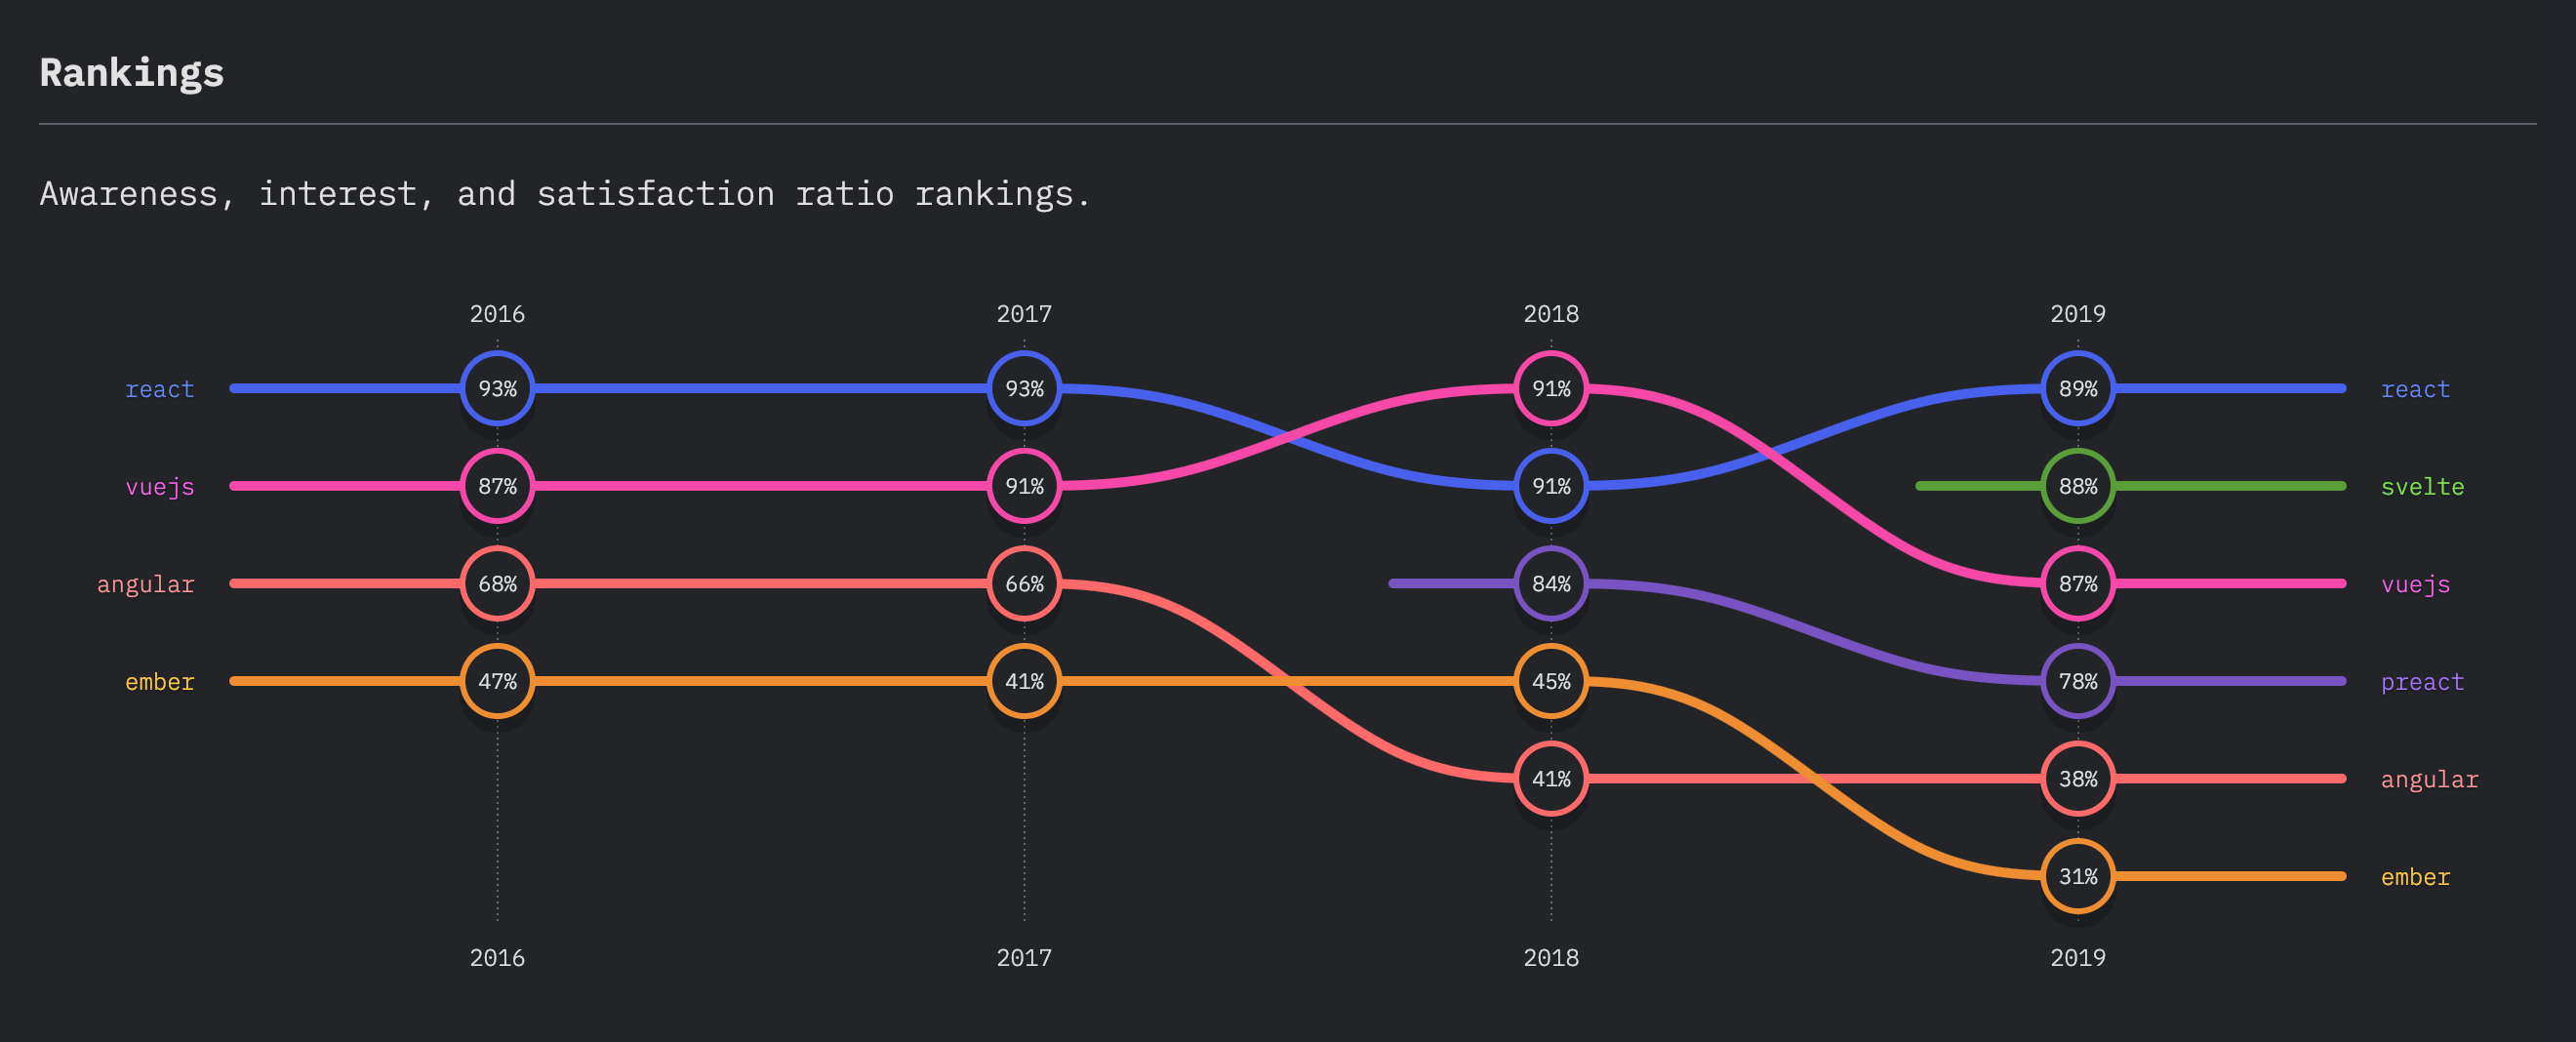
\includegraphics{front_end_frameworks_experience_ranking.png}
	\caption{2019 - Opinión popular de los entornos de trabajo front-end}
	\label{fig:stjs2019:frontend}
\end{figure}

\section{Entornos de trabajo del lado de servidor}
En esta sección se van a evaluar los entornos de desarrollo más populares en el lado del servidor teniendo en cuenta que se va a utilizar React. Si siguiésemos el mismo criterio que con el apartado del lado de cliente, encontraríamos que numerosas fuentes -por ejemplo, \cite{BKETPF1} y \cite{BKETPF2}- están de acuerdo en que PHP es la tecnología más utilizada en el lado de servidor con diferencia. Se puede apreciar en la figura \cref{fig:similartech:backend} sacada de \cite{BKETPF2} en Febrero de 2020. Sin embargo, en este caso particular y por la tecnología elegida en el lado del cliente, se van a valorar positivamente tecnologías que permitan desarrollar al mismo tiempo el cliente y el servidor. PHP es muy utilizado por varias razones:

\begin{enumerate}
	\item Es el más antiguo de los lenguajes de lado de servidor.
	\item Tiene la mayor comunidad que puede tener un lenguaje de servidor y, por tanto, una extensa documentación.
	\item Es utilizado por marcos aun más grandes, como Wordpress. Estos son \gls{cms} y están fuera del alcance de este proyecto.
\end{enumerate}

Sin embargo, PHP está pensado para directamente renderizar HTML, que es exactamente lo que hace React. Pese a que queremos dar soporte a las tecnologías más extendidas, también queremos estar actualizados con pilas tecnológicas que se están utilizando hoy para comenzar nuevos proyectos. Una de estas pilas tecnológicas de las que hablo es MERN (MongoDB, ExpressJS, ReactJS y NodeJS). Esta pila tecnológicas está recomendada por los siguientes motivos:

\begin{enumerate}
	\item Solo hay que aprender un lenguaje, Javascript, lo cual reduce la curva de aprendizaje.
	\item La gestión de datos internos de la aplicación es muy similar a la gestión de base de datos porque MongoDB trabaja con objetos Javascript.
	\item Se pueden hacer contenedores Docker que contengan la pila completa de forma muy sencilla, distribuyendo la carga y haciendo la aplicación escalable.
\end{enumerate}

Para esto se van a evaluar dos opciones: Express y Next.js. Se ha considerado utilizar múltiples entornos de servidor, entre ellos los que podemos encontrar en la figura \cref{fig:stjs2019:backend}. Sin embargo, teniendo decidido el lado del cliente, la mayoría de opciones no merecen la pena. React trabaja de forma estupenda con NodeJS y lo más habitual es que vayan de la mano. Además, como se ha comentado anteriormente, así se da soporte a la pila tecnológica que más está de moda. Entre Express y Next.js, la competición reside entre una librería ligera de desarrollo de las \gls{api} contra un entorno completo de \gls{ssr}. Durante el desarrollo del entorno se va a valorar abrazar ambas dos opciones como una configuración extra.

\begin{figure}
	\centering
	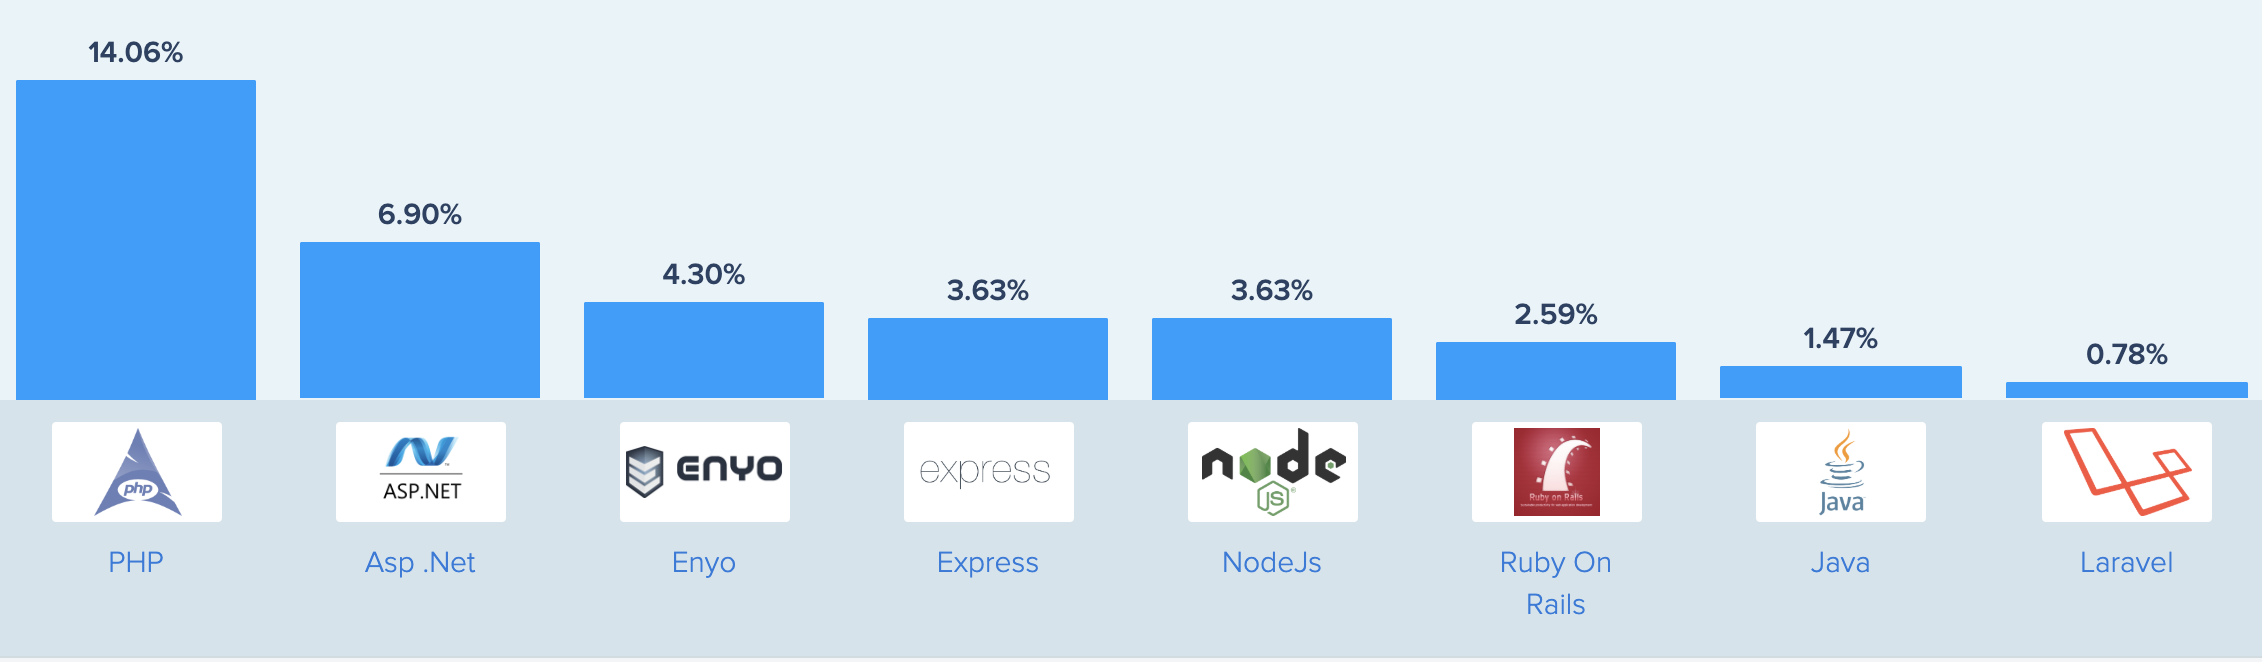
\includegraphics[width=\textwidth]{similartech_backend_trend_top_10K.png}
	\caption{Leading Framework technologies share on the web - Top 10K Sites}
	\label{fig:similartech:backend}
\end{figure}

\begin{figure}
	\centering
	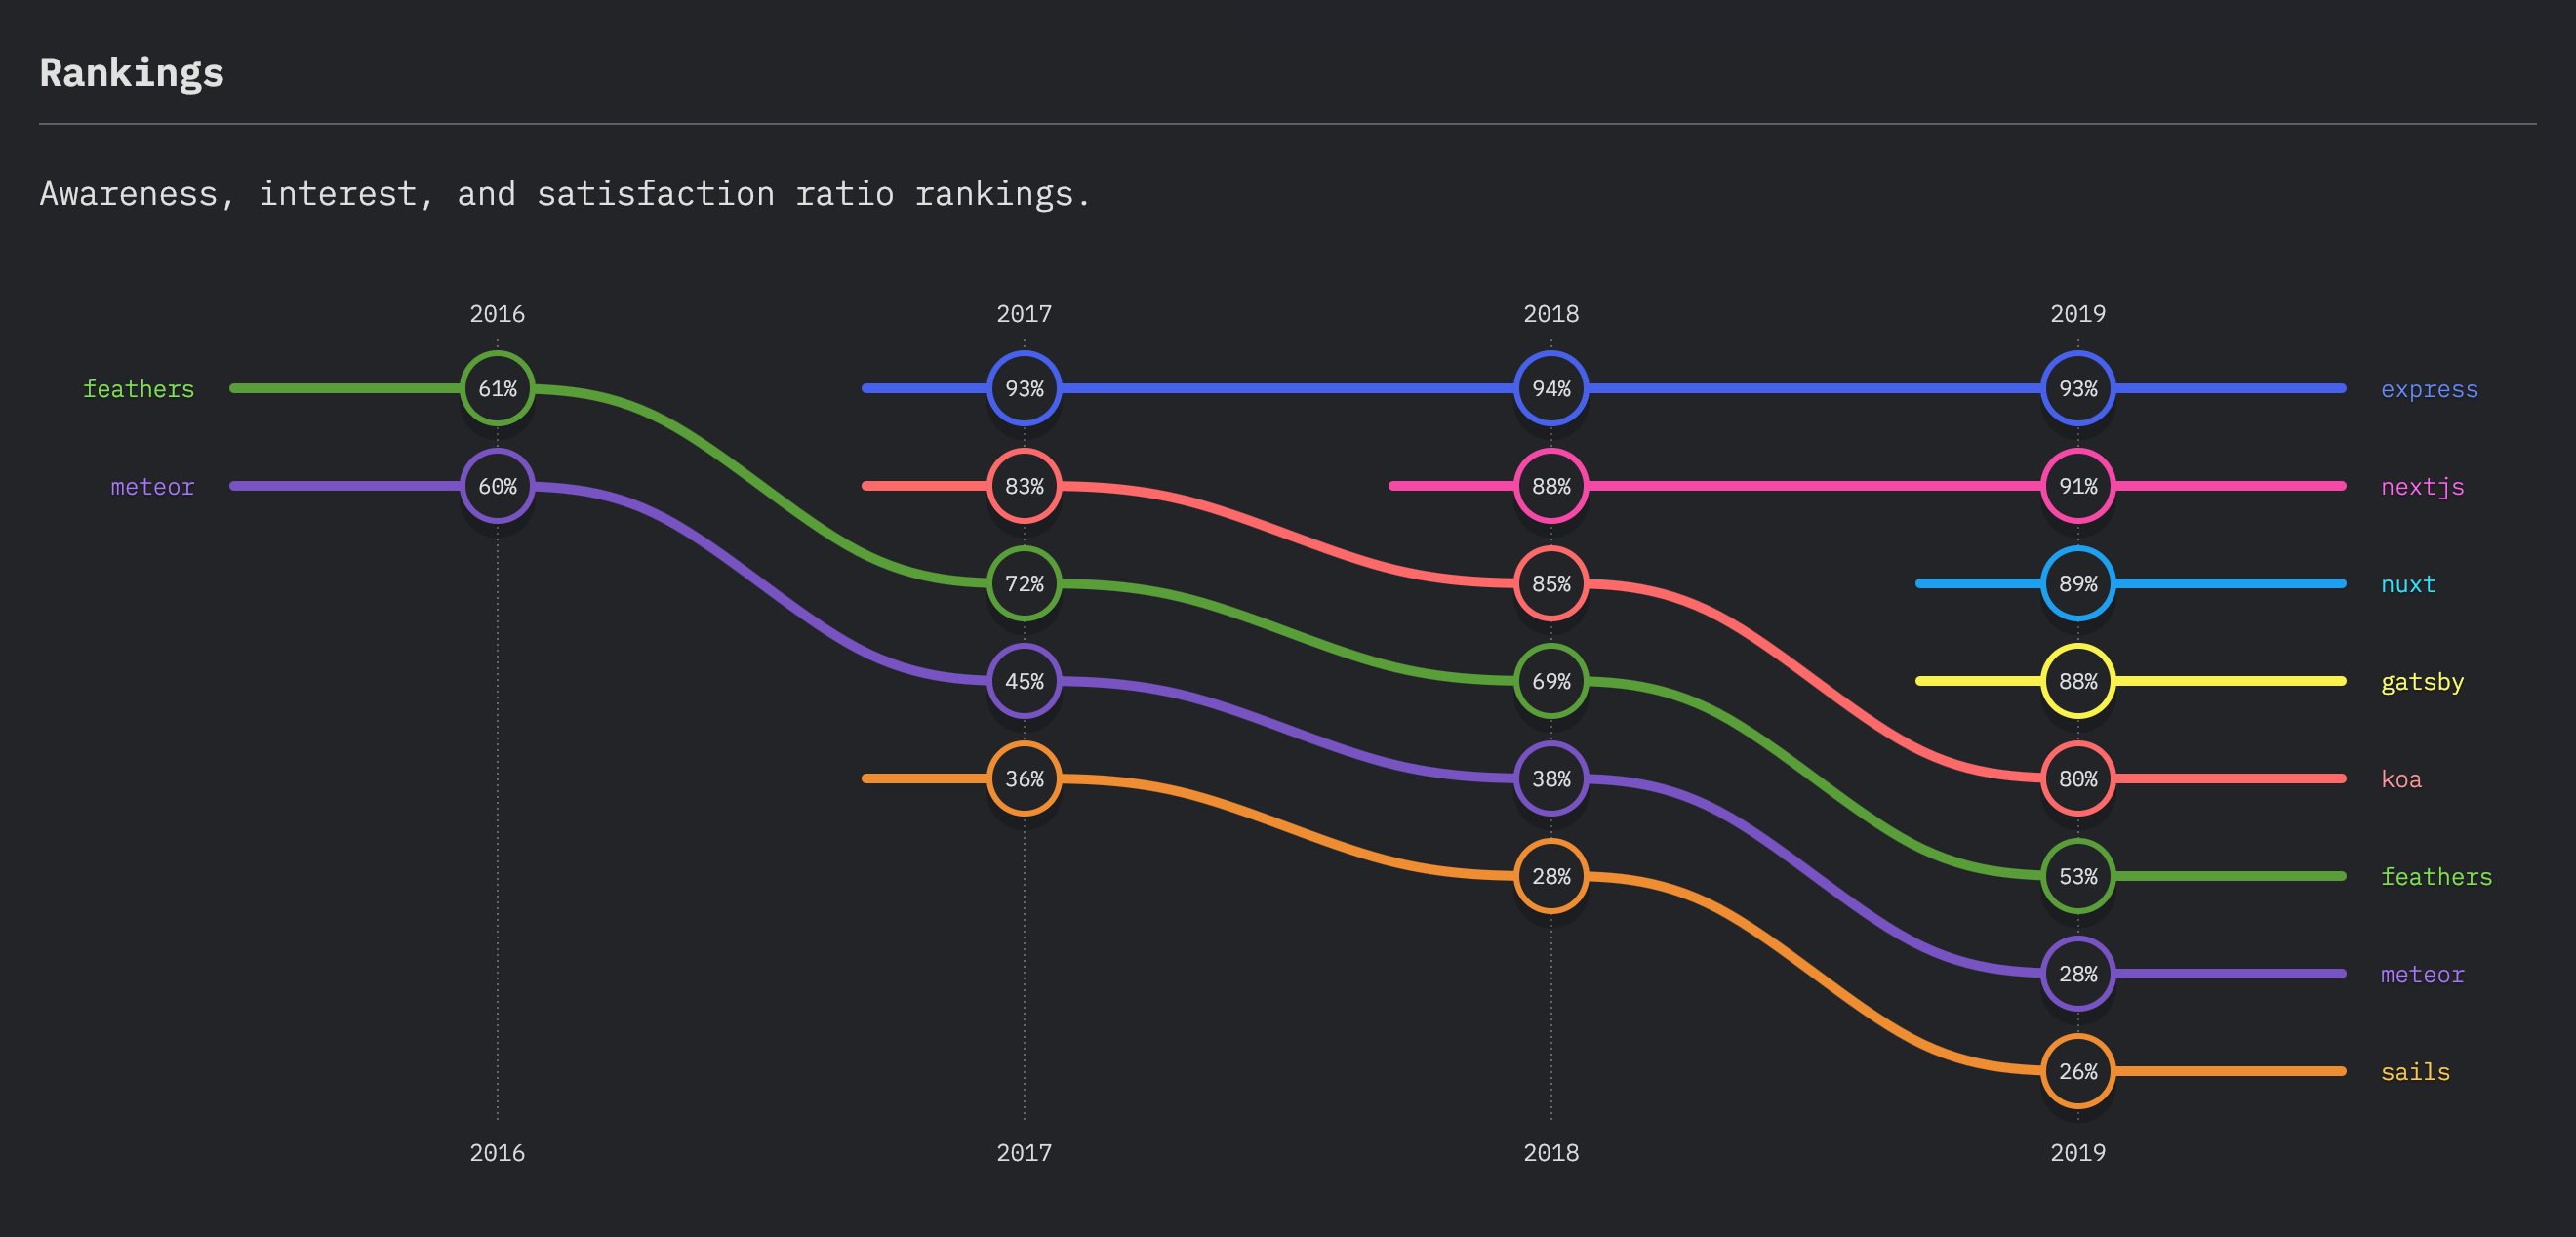
\includegraphics[width=\textwidth]{back_end_frameworks_experience_ranking.png}
	\caption{2019 - Opinión popular de los entornos de trabajo back-end}
	\label{fig:stjs2019:backend}
\end{figure}


\section{Control de versiones}
El control de versiones consiste en tener todas las versiones de código que se han generado etiquetadas, de forma que se pueda acceder a cualquier versión generada en cualquier momento. Esta es una base imprescindible para un proyecto de calidad, ya que permite trazar errores con mucha facilidad y es una salvaguarda ante fallos. Además, el control de versiones permite tener varias ramas de trabajo, separando el código de la rama de producción, la rama de desarrollo y las distintas ramas de los equipos y características que se están trabjando.

Hay muchas herramientas que permiten realizar este control de versiones y está sujeto a opinión cuál es mejor. Lo que no está sujeto a opinión es cuál se está utilizando más, lo cual se puede ver en gráficas como la figura \cref{fig:bd:source-control}, que nos facilita \citet{BDSRCMP}. Aparentemente el 70\% de los repositorios públicos está controlado mediante git. 

Otra ventaja de git es que es considerada la herramienta de alto rendimiento. Esto se puede ver también en la figura \cref{fig:g2:source-control}. El origen de esta figura, \citet{G2SRCMP}, nos permite además ir probando distintos parámetros, como el tamaño de la empresa. Y nos muestra que, en cualquier caso, git es la herramienta a elegir para el alto rendimiento.

Así que, con respecto al control de versiones, no hay duda de que git es la herramienta a elegir. Nos permite abarcar la mayoría de desarrollos públicos y es perfecto para el desarrollo de alto rendimiento que necesita un proyecto de calidad. Sin embargo, las decisiones no han acabado aquí. El control de versiones suele subirse a un servidor de repositorios -especialmente si pretende ser código libre-. Este proyecto va a ser código libre, de modo que se puedan proponer cambios y ramificar según distintas necesidades. Para esto, \citet{GHVSGL} explica de forma muy completa que, para proyectos de código abierto, Github es el que tiene mayor comunidad, así que va a tener com más facilidad una repercursión real.

Por tanto, han sido seleccionados git y Github para el control de versiones.

\begin{figure}
	\centering
	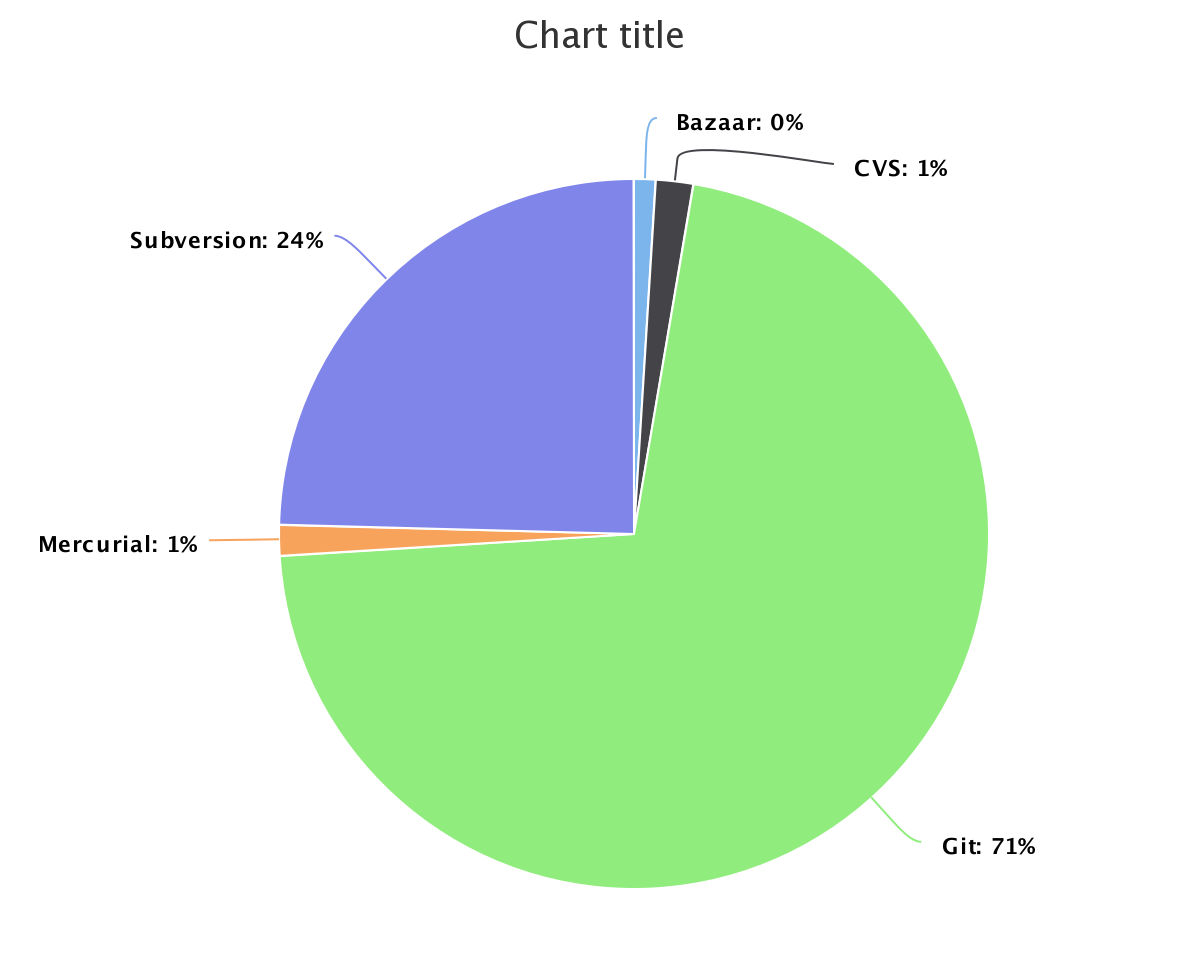
\includegraphics[width=\textwidth]{source-control.png}
	\caption{2019 - Compare Repositories}
	\label{fig:bd:source-control}
\end{figure}

\begin{figure}
	\centering
	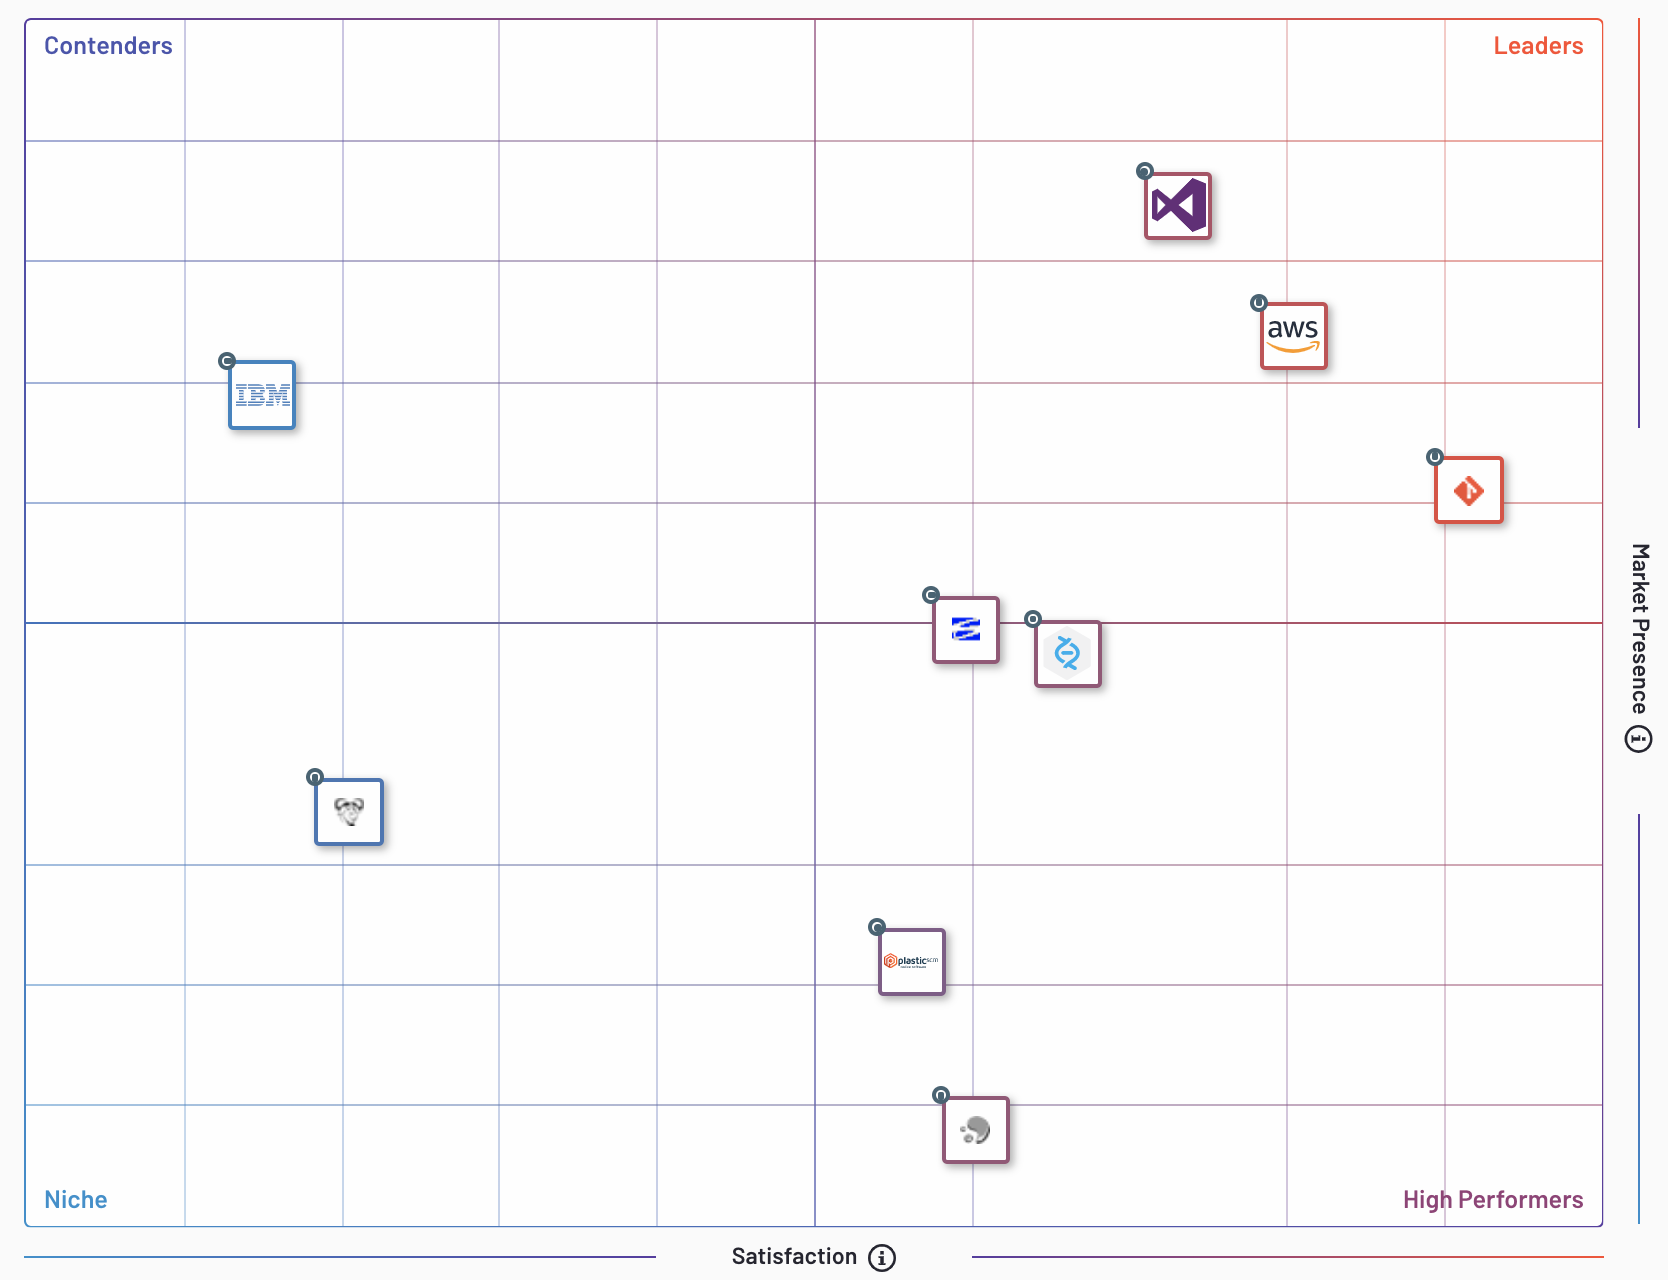
\includegraphics[width=\textwidth]{source-control-high-perf.png}
	\caption{2019 - Best Version Control Systems}
	\label{fig:g2:source-control}
\end{figure}

\section{Gestión de paquetes}
La gestión de paquetes consiste en el conjunto de herramientas que permiten descargar y mantener las dependencias que el proyecto va a utilizar. Como se ha decidido utilizar React + Express, el entorno de desarrollo es todo Javascript y, por tanto, en servidor se va a utilizar NodeJS, que tiene su propio gestor de paquetes: NPM.

Aunque NPM es una herramienta muy útil en su campo, no es la única que se ha creado para este propósito. Y hoy por hoy, la herramienta competidora por excelencia es Yarn. Como bien explica \citet{NPMVYRN}, existe una diferencia de velocidad a favor de Yarn (ver figura \cref{fig:package-manager:middle-size}). Sin embargo, \citet{NPMVYRN} también nos dice que esa diferencia de velocidad no es grande, así que no debería ser el motivo para elegir un gestor u otro. La funcionalidad de ambos gestores, pese a ser similar, tiene sus diferencias. Además, Yarn sacrifica espacio en disco para ganar ese extra de velocidad que NPM no tiene.

Como en este punto la decisión es tremendamente subjetiva y el coste de implementar ambos es pequeño, para este proyecto me voy a tomar la molestia de contemplar ambas opciones a la vez. Esto quiere decir que, en la configuración inicial del entorno, se presupondrá NPM (que es el gestor por defecto de Node), pero se permitirá al usuario cambiar a Yarn de forma sencilla y rápida.

\begin{figure}
	\centering
	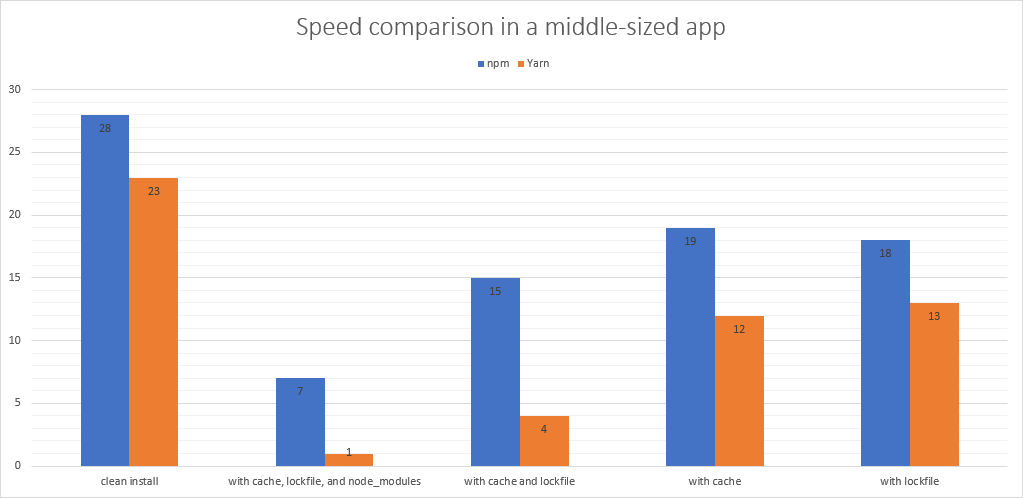
\includegraphics[width=\textwidth]{yarn-vs-npm-middle-sized-apps.jpg}
	\caption{NPM vs Yarn. Speed comparison in a middle-sized app}
	\label{fig:package-manager:middle-size}
\end{figure}

\label{section:packet-manager}

\section{Pruebas unitarias}
\label{section:unit-testing}
Las pruebas son una pieza esencial del código de calidad. Sirven para tener la certeza de que al usuario le llega siempre una versión de la aplicación que funciona como se espera. Hay tres tipos de pruebas: las unitarias, las de integración y las funcionales.

En concreto, las pruebas unitarias se encargan de comprobar que un componente de la aplicación funciona como se espera, independientemente del resto de componentes. Si se desea conocer más sobre las pruebas unitarias, recomiendo conocer la historia de \citet{WHYUNT}. 

En cualquier caso, cualquier aplicación con potencial de crecimiento necesita pruebas automáticas. En el mercado hay una infinidad de herramientas que nos resuelven este problema. Aunque en el caso de React, solo hay unas pocas que estén recomendadas oficialmente por el equipo de React. Como se especifica en la documentación (\cite{RETEUT}), se recomienda utilizar Jest junto con una de las siguientes librerías: React Testing Library o Enzyme. Jest parece la opción clara, dado que es la que utiliza Facebook (creadores de React), es la que más se utiliza en el mercado y es la que más satisfacción genera, como se puede comprobar en la figura \cref{fig:stjs2019:unit-testing}.

El dilema surge entre Enzyme y React Testing Library. ¿Qué diferencia hay entre ellos? Como primera respuesta, recomiendo leer la que ha dado \citet{EVRUVRL} en Stack Overflow. Básicamente, Enzyme nos permite acceder a los métodos de nuestros componentes y React Testing Library siempre simula el componente completo. Además, Enzyme permite algo llamado Shallow Render. Esto significa dibujar únicamente el componente que se desea probar, simulando sus hijos. Enzyme es más fácil de utilizar, pero más peligroso y, a la larga, menos mantenible. El hecho de que React Testing Library nos obligue a utilizar los componentes tal y como se renderizan en un ambiente de producción implica tener más seguridad en nuestro código, tal y como explica \citet{NVSHRD} en su artículo y, posteriormente, revisa \citet{RVRT19} en 2019. La filosofía es sencilla: es mejor hacer pruebas que den la confianza de que el código funciona y no emularlo.

Por estos motivos, las pruebas unitarias van a ser mediante Jest y React Testing Library, que son las herramientas recomendadas oficialmente. Durante el transcurso de este trabajo, se valorará utilizar Enzyme haciendo comprobaciones sobre la curva de aprendizaje y la velocidad en proyectos más pequeños, pudiendo ser implementado como opción. Sin embargo, como este entorno pretende ser útil en proyectos con potencial de crecimiento, se preferirá el uso de React Testing Library por su mejor mantenibilidad.

\begin{figure}
	\centering
	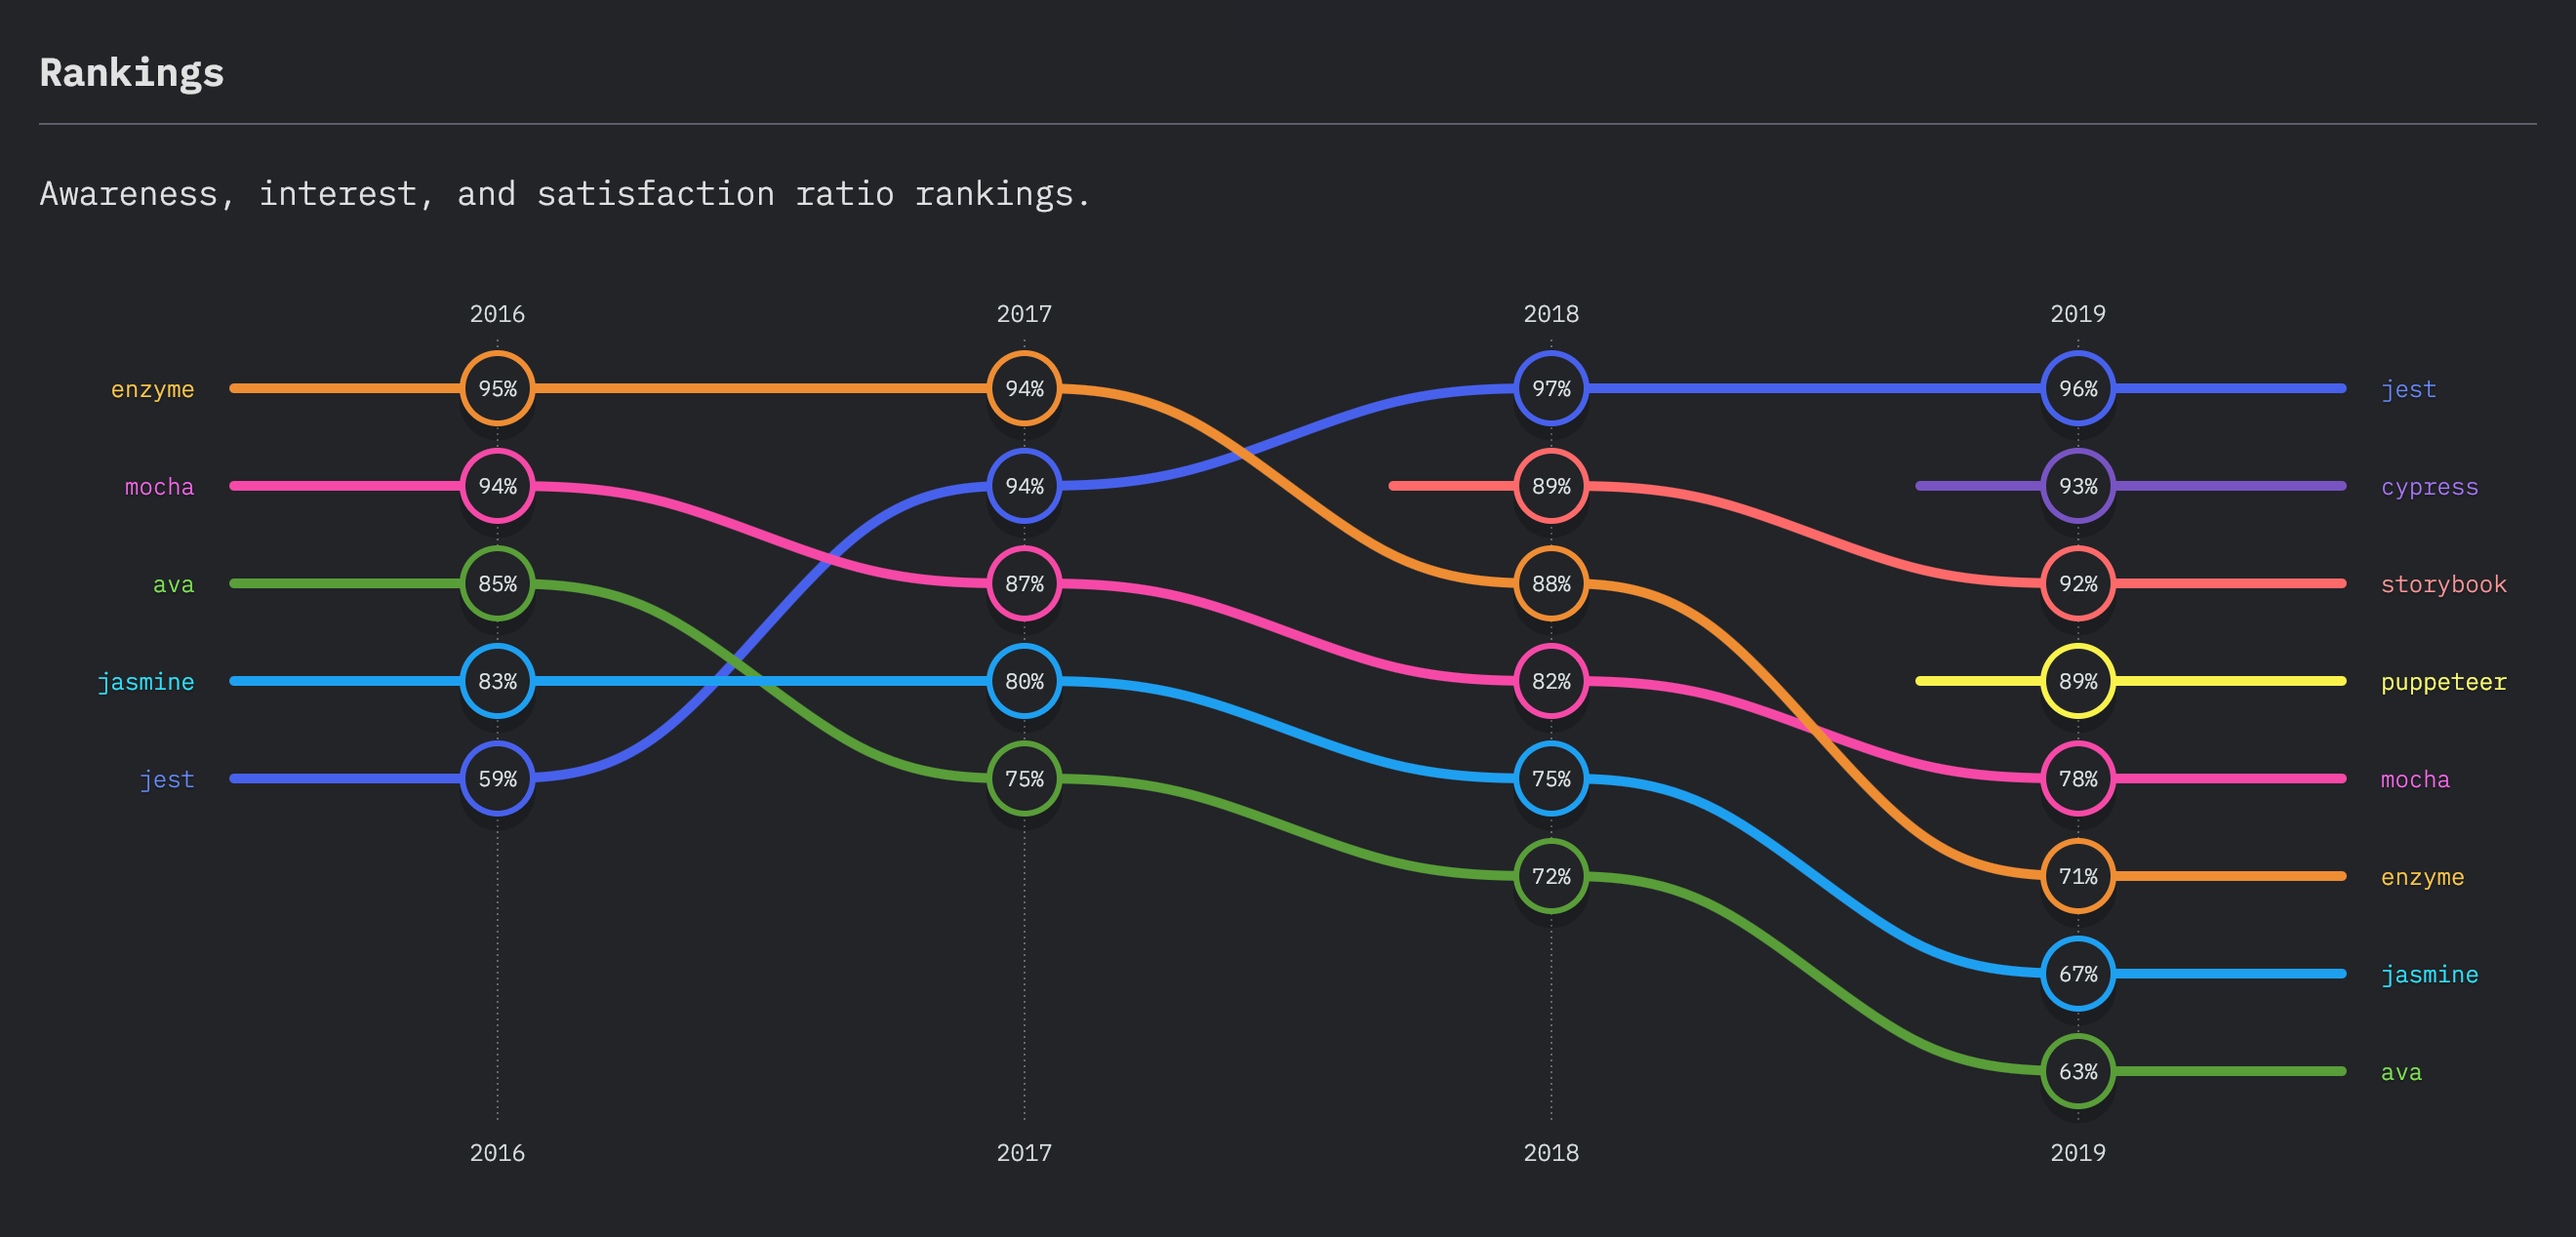
\includegraphics[width=\textwidth]{testing_experience_ranking.png}
	\caption{2019 - Opinión popular de las herramientas de pruebas unitarias}
	\label{fig:stjs2019:unit-testing}
\end{figure}

\section{Pruebas de integración}
\label{section:integration-testing}
Las pruebas de integración son aquellas pruebas que permiten comprobar de forma automática que un componente de la aplicación está funcionando bien cuando se utiliza junto con otro componente. Es posible que dos componentes funcionen correctamente cuando están aislados, pero en el momento en el que se unen ocurre funcionalidad inesperada. Las pruebas de integración permiten detectar este fenómeno para poder alertar al desarrollador. Si se desea conocer más sobre las pruebas de integración, recomiendo visitar \citet{DZITWH}.

Durante las pruebas unitarias, hemos hablado de dos librerías de pruebas en React: Enzyme y React Testing Library. De hecho, gran parte de la discusión se ha centrado en un tema que, pese a que no tocaba en ese momento, era indivisible del resto de la comparación. El motivo por el que se ha elegido React Testing Library sobre Enzyme es porque es más preciso en las pruebas de integración. De hecho, Enzyme no realiza pruebas de integración dado que simula la generación de los hijos de un componente.

Así que en React las pruebas de integración y las de unidad están íntimamente relacionadas. Las unitarias se encargarían de comprobar la funcionalidad dentro de un componente React y las de integración, ver cómo se comportan los componentes hijos dentro de distintos componentes padre. En cualquier caso, tal y como nos dice \citet{RECTIT}, las librerías de pruebas unitarias y de integración son las mismas: Jest y React Testing Library.

\section{Pruebas funcionales}
\label{section:e2e-testing}
Las pruebas funcionales o \gls{e2e}, son aquellas pruebas que son totalmente agnósticas de la tecnología utilizada para desarrollar la aplicación. Se encargan de interactuar con ella como si fuesen el usuario final. En el caso de las aplicaciones web, se suelen utilizar navegadores de tipo Headless para realizar estas pruebas de forma automática. Estas pruebas son totalmente independientes de React y NodeJS, aunque lo ideal es desarrollarlas en el mismo lenguaje que el resto de pruebas que se realizan en la aplicación.

Para decidir qué herramienta de pruebas \gls{e2e} se va a utilizar, se han considerado las citadas en el artículo \cite{MPSFT19}. Dentro de estas, se han descartado todas ellas que no tienen compatibilidad con NodeJS para el desarrollo de los casos de prueba o aquellas que no tiene una versión gratuita. Así que se han tenido en cuenta únicamente Selenium y Crypress.

Tal y como explica \citet{CYPVSEL}, Selenium es una herramienta madura y estable, con mucha funcionalidad y que tiene configuración algo más pesada. Sin embargo, Selenium permite grabar las acciones que se realizan sobre el navegador y generar los casos de prueba automáticamente. Y esto es exactamente lo que interesa al marco de trabajo que se propone: ser de configuración rápida y fácil uso para una aplicación pequeña. De la configuración se encargará el propio marco, así que la capacidad de grabar el navegador es una gran ventaja con respecto a Cypress. Además, Selenium está preparado para trabajar con Jest.

Por otro lado, Cypress está específicamente diseñado para entornos de NodeJS y está creciendo a gran velocidad. Como sugiere \citet{CYPVSEL}, Cypress debería considerarse como una alternativa a futuro, que según vaya creciendo se puede ir incorporando a este proyecto. Hoy por hoy, Selenium es líder en herramientas de pruebas \gls{e2e} y, con todo el apoyo que da a entornos de Javascript y Node, no hay ninguna otra que sea apropiada para la tarea.


\section{Gestor de Base de Datos}
Esta decisión es probablemente la más difícil de todas las que se han tomado en este proyecto. Por un lado, la gestión de bases de datos depende mucho de los conocimientos técnicos del desarrollador. Por otro, la base de datos puede acelerar mucho el tiempo de desarrollo en función de la afinidad que haya entre los datos y el gestor elegido. Además, hay gestores que son más escalables o tienen distintas prestaciones en función del resto de tecnologías elegidas.

Para tomar esta decisión, se han abordado los puntos con sumo cuidado, comenzando por un análisis de popularidad, tal y como se ha hecho en las anteriores secciones. Según el análisis de \citet{MPDBITW} (resumido en la figura \cref{fig:dbms}), los gestores de bases de datos más populares son:
\begin{enumerate}
	\item Oracle
	\item MySQL
	\item Microsoft SQL Server
	\item PostgreSQL
	\item MongoDB
\end{enumerate}
Las cuatro primeras opciones son todo bases de datos relacionales. En quinta posición se encuentra MongoDB, que es la única opción no relacional dentro del top de popularidad. Como uno de los objetivos de este marco es llegar al mayor número de desarrolladores posible, se ha intentado mantener el marco dentro de estos gestores de bases de datos. Además, otro factor a tener en consideración es que no se va a incluir ninguna herramienta que no sea gratuita, así que Oracle y Microsoft SQL Server quedan descartadas. Esto reduce las posibilidades a tres gestores de base de datos: MySQL, PostgreSQL y MongoDB.

MySQL y PostgreSQL son, como comenté, bases de datos relacionales que utilizan un lenguaje común: \gls{sql}. Además, hay otros muchos gestores que utilizan este lenguaje de consultas y cada usuario puede preferir uno u otro. Hay una discusión abierta sobre cuál es mejor y hay defensores y detractores de cada uno. Se puede leer un poco más de este tema en la reflexión de \citet{MYSVPOS}.

MongoDB es un gestor no relacional (en concreto, se le conoce como lenguaje No \gls{sql}). Esto quiere decir que no se basa en un modelo estricto. Específicamente, MongoDB es un \gls{dod}. Se puede leer más sobre este tipo de gestores en la propia documentación de MongoDB (\cite{DOCORDB}). Lo que hace a MongoDB tan buen gestor de base de datos para entornos NodeJS es que esos documentos que gestiona se guardan en formato \gls{bson}, que es una forma de guardar en disco de forma eficiente documentos \gls{json}. La forma de comunicarse con este gestor es enviando precisamente objetos con exactamente la misma sintaxis que los objetos en JavaScript. Así que es un lenguaje estupendo para trabajar desde entornos con JavaScript.

Por otro lado, hay que tener en cuenta los \gls{orm}, que son herramientas que hacen de capa intermedia entre la aplicación y la base de datos. Permiten modelizar los datos como si fuesen objetos y se encarga de mantener la coherencia entre la base de datos y la estructura proporcionada. Realizar operaciones básicas es muy directo utilizando un \gls{orm}, pero aumentan la dificultad y reducen la eficiencia de operaciones complejas. Por tanto, utilizar o no un \gls{orm} depende mucho de las necesidades de la aplicación. Se puede leer más sobre los criterios de utilización de un \gls{orm} en los artículos de \citet{ORMYON1} o \citet{ORMYON2}. Sin embargo, los \gls{orm} permiten utilizar la misma sintaxis para comunicarse con bases de datos diferentes, lo cual es algo que beneficia mucho a un marco de lanzamiento rápido como se está desarrollando. Si buscásemos a un \gls{orm} adecuado, TypeORM podría ser un ORM adecuado porque tiene soporte a MySQL, PostgreSQL y MongoDB a la vez.

Como se puede comprobar, cada tecnología en este apartado tiene sus ventajas e inconvenientes. Modelos relacionales permiten una estructura consistente en base de datos, mientras que MongoDB permite introducir en la base de datos objetos que tiene guardados en su memoria interna sin ninguna transformación. Por otro lado, el modelo puede requerir otros tipos de gestores. Los datos podrían requerir otros modelos (ver artículo de \citet{DBMSTYP}) o los desarrolladores podrían estar más familiarizados con algún otro en particular. Es importante recalcar que no debería ser tarea del marco elegir la tecnología que debería utilizar el usuario para la permanencia de información. Sin embargo, sí que es tarea del marco reducir al mínimo el tiempo que emplea un usuario en la configuración inicial del entorno. El marco está principalmente orientado a la calidad de código. Esto puede conseguirse independientemente del gestor de base de datos elegido.

Por todo esto, se ha decidido que el marco va a dar soporte a una configuración rápida para un entorno con MySQL, PostgreSQL, MongoDB o TypeORM. Será una opción, se gestionará localmente en la máquina que está preparada para alojar el proyecto y siempre será un elemento de libre configuración. De este modo, si la aplicación no necesita permanencia de datos o necesita una más especializada, el marco no pondrá límites en este aspecto.

\begin{figure}
	\centering
	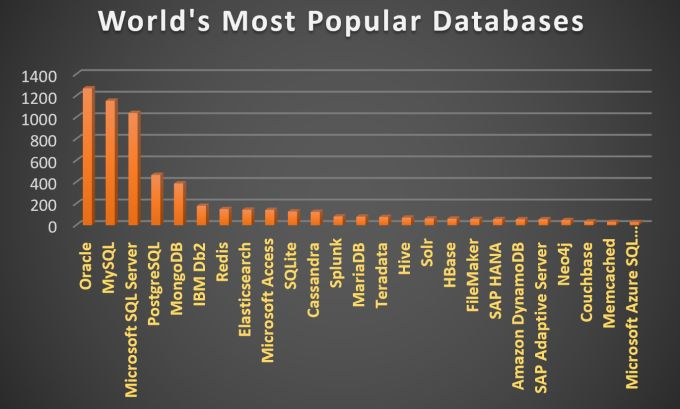
\includegraphics[width=\textwidth]{popular_databases.jpg}
	\caption{2019 - Most Popular Databases In The World}
	\label{fig:dbms}
\end{figure}

\label{section:database-manager}

\section{Capa de datos}
La persistencia de datos es muy importante de cara a mantener una aplicación web. Sin embargo, en los marcos de trabajo actuales, es habitual descargar mucha carga de datos en el cliente y que este lo vaya administrando. Esta gestión puede ser muy tediosa si no se utilizan unas tecnologías llamadas capas de datos, que permiten mantener la coherencia de los datos en toda la aplicación. Las herramientas más populares se muestran en la Figura \cref{fig:stjs2019:datalayer}. 

Se puede apreciar que GraphQL es líder en este sector, y no por pocos motivos. Esta herramienta fue creada por Facebook (al igual que React y su principal competidora, Redux) y ha nacido a raíz de algunos problemas que surgían al utilizar React. Sin embargo, no está diseñada exclusivamente para React. GraphQL se puede utilizar junto con cualquier entorno. Dado que esta herramienta es la más popular en el mercado, está diseñada por los creadores de React y resuelve los problemas que explica \citet{RDXVGQL} en su artículo, es la herramienta elegida para el marco que se ha desarrollado.

Sin embargo, no siempre se necesita capa de datos en el cliente y, por tanto, la posibilidad de utilizar GraphQL será una configuración opcional. En la configuración inicial, al desarrollador se le preguntará si desea capa de datos (GraphQL) en su entorno y este podrá sencillamente contestar si lo desea o prefiere desarrollar su producto controlando la capa de datos de forma personalizada, ya sea mediante otra herramienta o cuidando el estado y las propiedades de sus componentes de React.

\begin{figure}
	\centering
	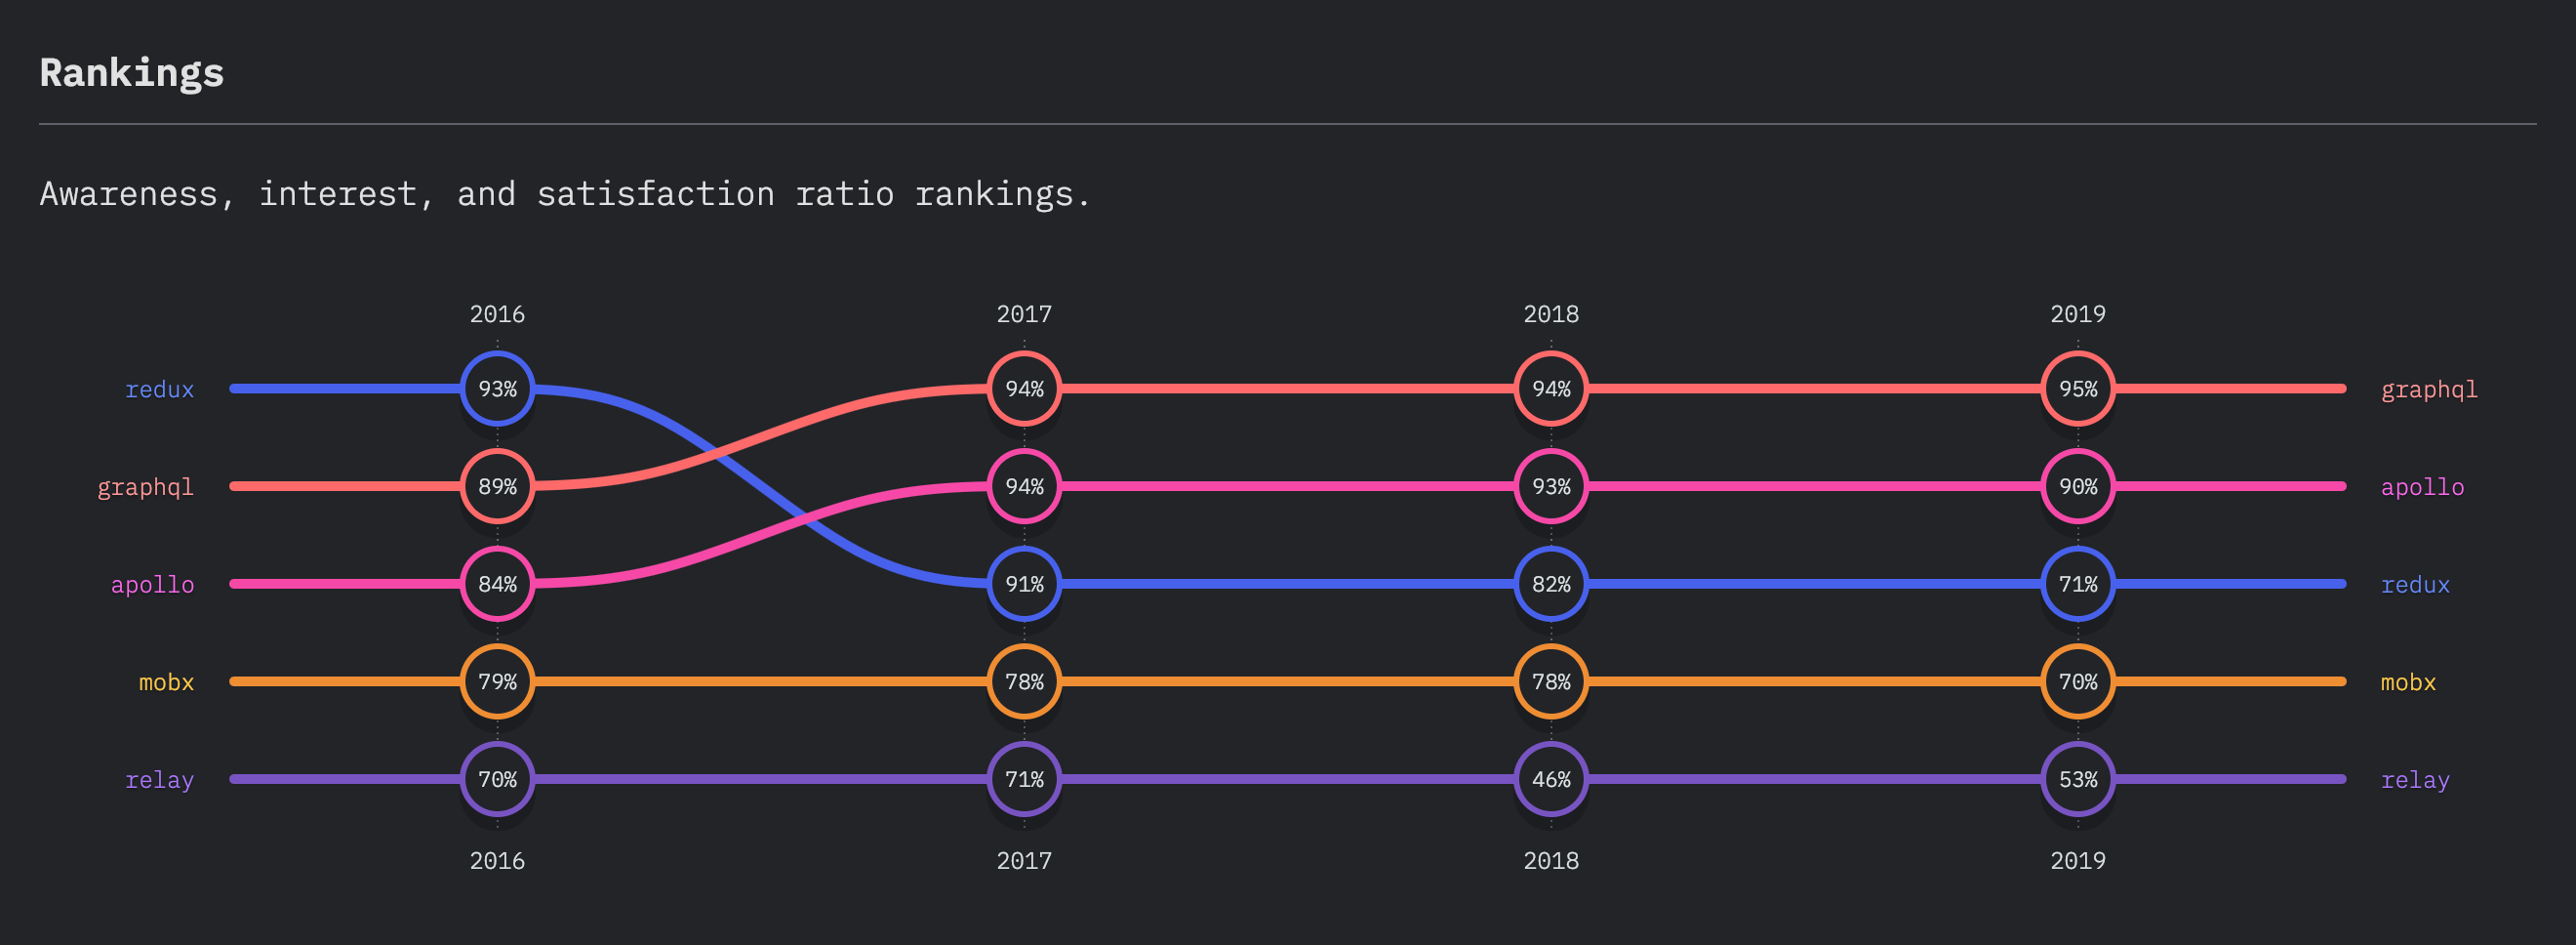
\includegraphics[width=\textwidth]{data_layer_popularity.png}
	\caption{2019 - Opinión popular de las herramientas de gestión de la capa de datos}
	\label{fig:stjs2019:datalayer}
\end{figure}

\label{section:data-layer}

\section{Flujo de despliegue - Integración continua}
\label{section:ci-cd-flow}
La integración contínua es una disciplina que permite automatizar el flujo de código desde el momento en que un desarrollador lo genera hasta que llega a la rama principal de código del repositorio, asegurando por el camino que es código de calidad mediante pruebas automáticas mencionadas en las secciones \nameref{section:unit-testing}, \nameref{section:integration-testing} y \nameref{section:e2e-testing}. Además, uniéndolo con el despliegue contínuo, se puede lograr que haciendo solo un click el código sea verificado, enviado a un servidor y expuesto al público. \citet{CVTRVJK} explica este procues en su artículo, mostrando además dos gráficos muy representativos de cómo funcionan la integración contínua (\cref{fig:ci}) y el despliegue contínuo (\cref{fig:cd}).

En la figura \cref{fig:ci} se puede observar cómo múltiples desarrolladores pueden colaborar simultáneamente enviando sus aportaciones a un servidor de control de versiones como GitHub. Mediante un simple evento PUSH en una rama de desarrollo, los cambios irán al repositorio, que emitirá la nueva versión a un servidor de integración contínua. El servidor verificará que el código cubre todos los casos de prueba y, en caso de fracasar, notificará a los desarrolladores involucrados en la nueva versión, que podrán arreglar los fallos y volver a intentar una subida. En caso de éxito, podrá notificar a los desarrolladores también. Sin embargo, lo más habitual es que un éxito desencadene el siguiente proceso, el despliegue contínuo, que se encargará de subir la nueva versión a un servidor público de forma inmediata. Cabe remarcar que este servidor público puede estar duplicado (uno para desarrollo y otro para producción), generando dos procesos de integración contínua que pueden estar tanto encadenados como construidos de forma independiente.

En la figura \cref{fig:cd} se muestra el proceso completo, incluyendo la integración contínua y el despliegue contínuo. En este flujo pueden intervenir revisiones manuales de código y pruebas por parte de los usuarios. Este proceso asume que la aplicación es desarrollada en un entorno profesional, pero el marco que se plantea desarrollar no está pensado en un ámbito de empresa. El marco pretende abarcar proyectos pequeños (de pocos desarrolladores) con potencial de crecer. Por tanto, este flujo debe tenerse en consideración, pero no debe ser la principal preocupación del marco.

La idea es que el marco proporcione de forma sencilla tanto un entorno de integración contínua como un entorno de despliegue contínuo. Es objeto de estudio de este marco analizar las distintas herramientas que permiten hacer estas tareas y pensar en cómo podría un proyecto escalar a ámbito profesional sin modificar las herramientas que se utilizan en el proceso. Para poder realizar estas tareas, se han analizado las dos herramientas gratuitas que propone \citet{CVTRVJK}: Jenkins y CircleCI. TravisCI se descarta por su carácter de pago, que rompe con la filosofía del marco.

\begin{figure}
	\centering
	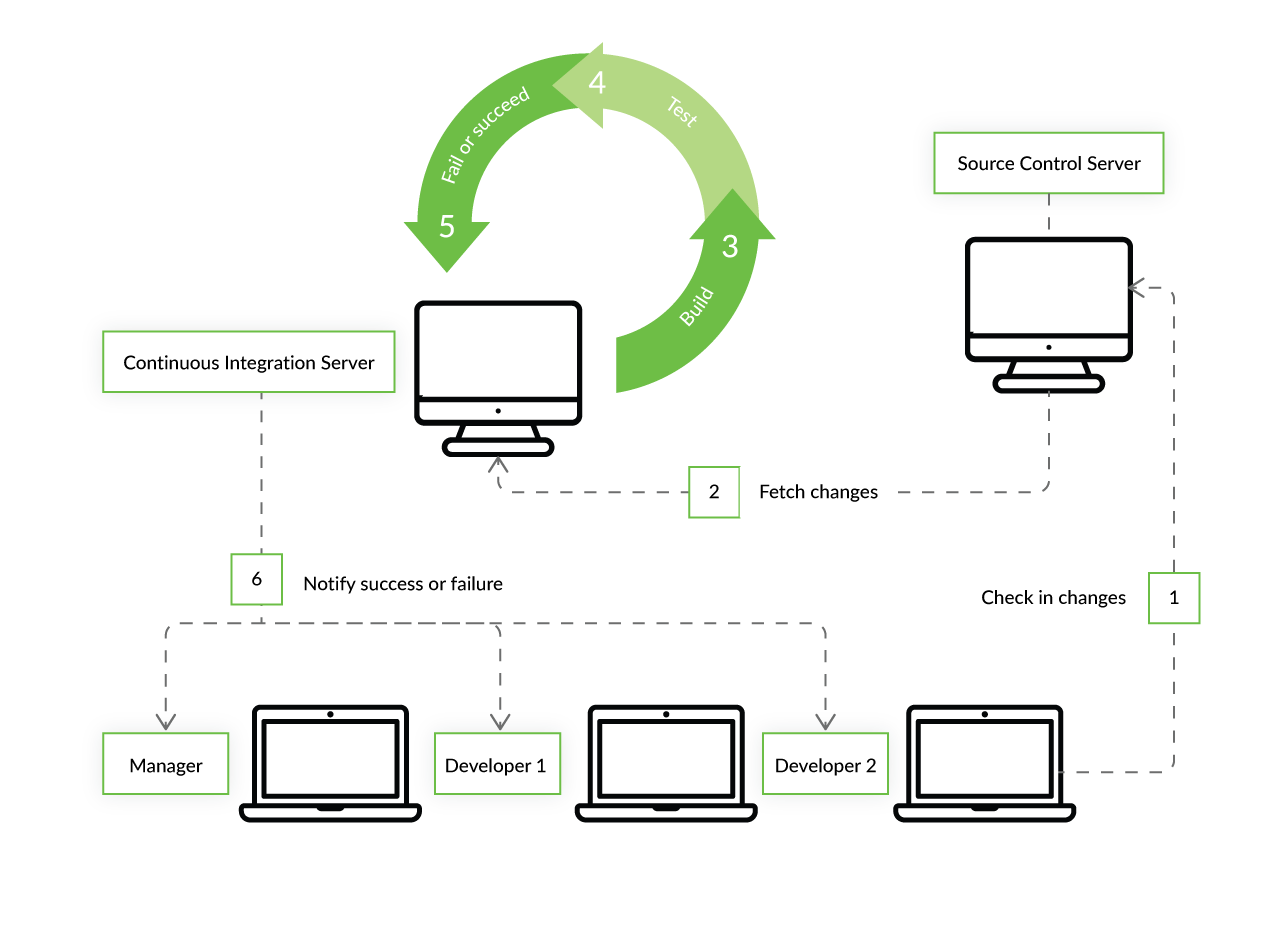
\includegraphics[width=\textwidth]{how-ci-works.png}
	\caption{How Continuous Integration Works}
	\label{fig:ci}
\end{figure}

\begin{figure}
	\centering
	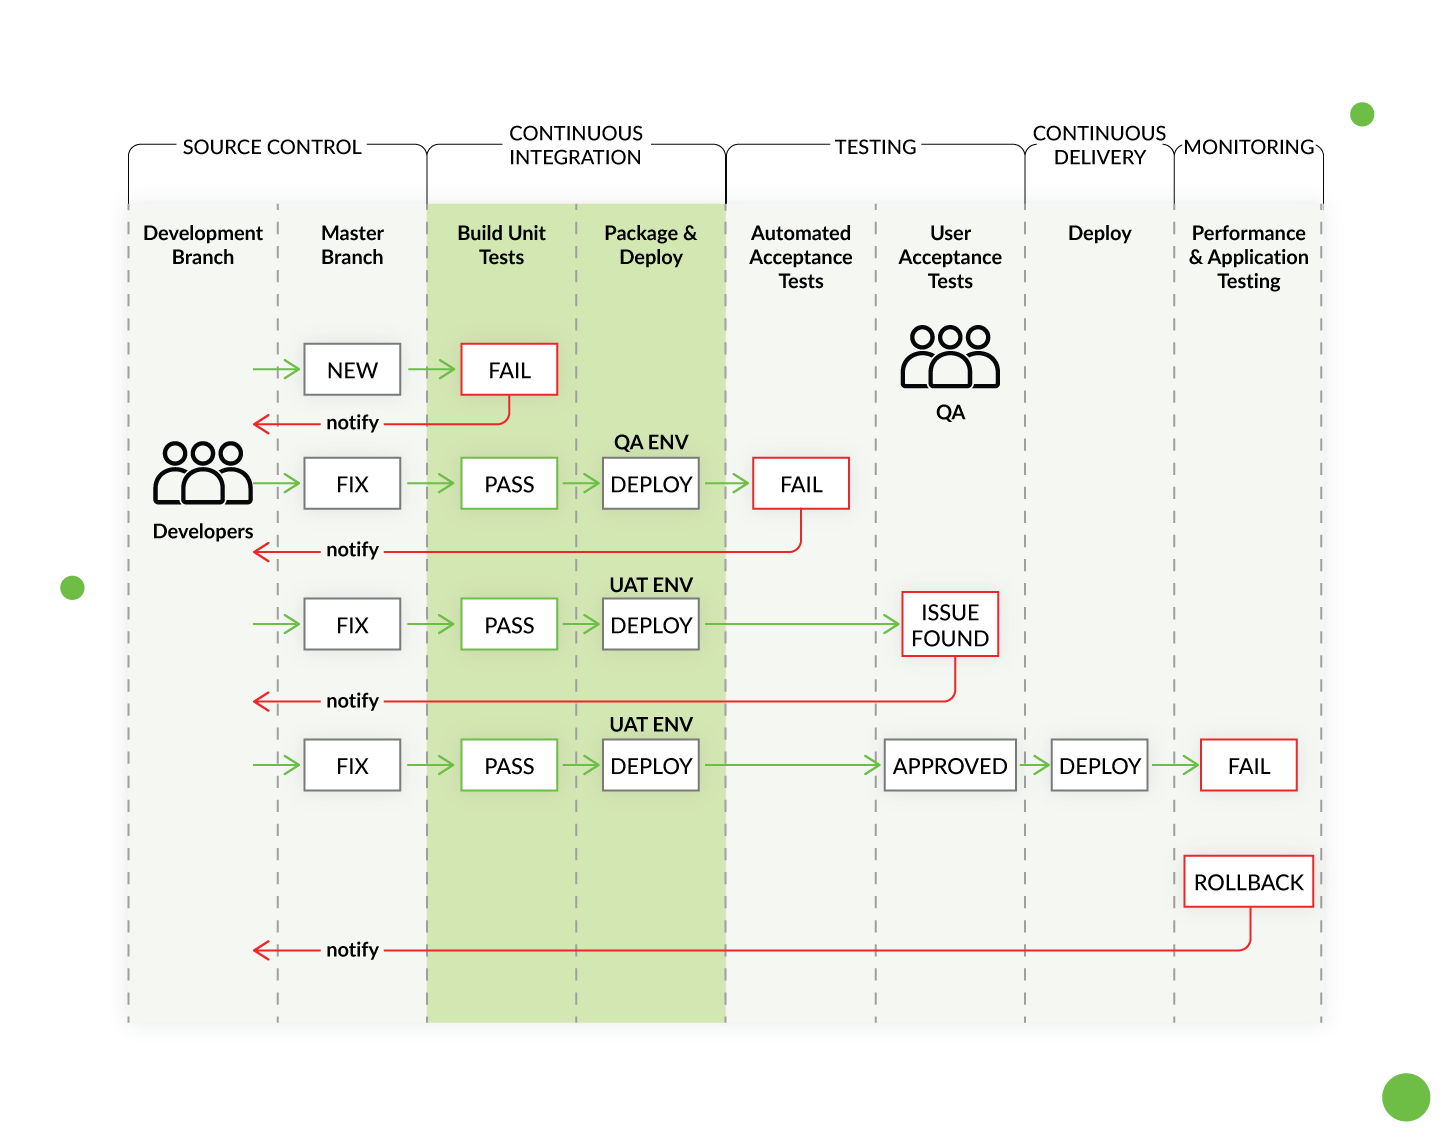
\includegraphics[width=\textwidth]{release-workflow.png}
	\caption{Release Workflow}
	\label{fig:cd}
\end{figure}


\chapter{Definición del Problema}
Tal y se ha explicado en el capítulo de \nameref{chap:state-of-art}, existen numerosas tecnologías que nos permiten hacer un proyecto de formas distintas. Cada una de ellas tiene sus ventajas e inconvenientes y unas son más populares que otras, pero todas tienen un coste de aprendizaje. En un proyecto de desarrollo web, hace falta dedicar un esfuerzo a generar la infraestructura necesaria para poder utilizar la tecnología. A veces es instalar un paquete, a veces es crear un módulo de código, otras veces es preparar unos procesos en el fichero de definición de proyecto y otras instalar un programa. Entre el tiempo que se dedica a investigar, el tiempo que se dedica a hacer pruebas con la nueva tecnología y el tiempo que se dedica a resolver errores el tiempo de configuración puede resultar ser incluso mayor al tiempo de desarrollo en proyectos pequeños. A esto hay que sumarle que no siempre es trivial resolver interacciones entre distintas tecnologías, como por ejemplo interacciones entre Jenkins y Github o entre Apollo y React.

Es muy fácil olvidar la calidad de código cuando hay una fecha límite para crear el proyecto y se dedica tanto tiempo a jugar con las líneas de código hasta que el resultado es el esperado. Es muy frecuente encontrar marcos de trabajo para una pila concreta de tecnologías que solucionan el problema, pero son todo marcos de trabajo independientes y muchas veces también con filosofías de desarrollo distintas, así que es complicado encontrar dos marcos de trabajo compatibles. En muchas ocasiones no tienen incluidas las pruebas o tienen ligeras variaciones sobre la pila de tecnologías necesarias.

He comentado el concepto calidad de código anteriormente: estamos considerando código de calidad a aquél que siga las buenas prácticas, sea mantenible, se pruebe automáticamente y aproveche la integración y la implementación continuas. A continuación voy a ir desgranando estas condiciones para su mejor comprensión.

Un código que sigue buenas prácticas es aquél que se basa en un estándar corporativo y, por tanto, todos sus desarrolladores escriben código que tiene forma similar. Generalmente, el estándar corporativo se alinea con un estándar que ha ido generando la comunidad de desarrolladores del lenguaje en cuestión a base de experiencia. Quizá un lenguaje particular dispone de una herramienta que, al utilizarla, la experiencia dicta que genera más problemas que soluciones, así que es preferible evitar su uso. En otras ocasiones, las buenas prácticas establecen los criterios de nombrado de variables, el tipo de indentación, la información que se espera ver en los comentarios y qué comentarios se esperan ver en cada módulo. Las buenas prácticas tienen el mismo objetivo que las pruebas automáticas: evitar errores. No todas las buenas prácticas son evaluables por procesos automáticos, pero la mayoría sí lo son. Y esos procesos automáticos requieren una configuración. Sería cómodo poder evitarse este tiempo si se asume que todos los proyectos van a escribirse a los estándares de la comunidad de desarrolladores de Javascript y se utilizan todos los procesos automáticos validados por la comunidad para forzar la aplicación de estas buenas prácticas.

Un código mantenible es aquél que, a medida que escala en tamaño, sigue siendo fácil conocer la función de cada parte y se puede mantener independiente cada módulo. Es muy difícil librarse de todas las dependencias entre modulos, pero al fin y al cabo el código es mantenible mientras sea fácil identificar qué hace cada módulo de forma independiente. Es importante mantener un orden en el directorio de ficheros y un sistema de nombrado apropiado. Es por eso que la estructura del proyecto debe estar pensada de antemano en base de las tecnologías que se vayan a utilizar y, asimismo, la estrcutura debe estar preparada para recibir ampliaciones. Todo este esfuerzo de planificación no tiene por qué hacerse en cada nuevo proyecto, dado que es muy probable que una estructura particular encaje en todos los proyectos que compartan un conjunto dado de tecnologías. Es por eso que en la comunidad de desarrolladores se han ido generando estructuras para los conjuntos de tecnologías más habituales que están validadas por al experiencia. Sería bueno poder evitarse ese proceso de diseño sabiendo que ese conocimiento existe en la comunidad.

Además, el código es mantenible si modificar un módulo no tiene riesgo de generar un error en un módulo distinto. Para esto, se ha creado el apartado específico de las pruebas automáticas. Todo código que se cree debe estar soportado por una batería de pruebas que se encargarán de generar una alerta cuando el código deje de hacer lo que debería. Esas pruebas hay que escribirlas y suponen un esfuerzo inevitable. No existe proceso automático que entienda las necesidades de negocio de un proyecto y las traduzca a pruebas automáticas, pero sí que existen algunas pruebas automáticas independientes de las necesidades de negocio como el análisis de imágenes instantáneas del producto. Este tipo de pruebas avisan en caso de que el producto cambie de forma, y es responsabilidad del desarollador analizar si ese cambio en la instantánea era esperado o no. Con todo y con eso, las pruebas automáticas requieren configuración y estructura y dependen de las tecnologías implicadas. Así que un proceso automático sí podría encargarse de, dadas unas tecnologías, generar dichas estructura y configuración necesarias para poder escribir casos de prueba. Todo esto se ha comentado y explicado más en detalle en el apartado de \nameref{section:unit-testing}.

Por último, la integración contínua. Muchas veces queremos tener el producto en un lugar accesible, queremos protegerlo de versiones defectuosas, queremos tener una versión del producto de desarrollo para poder actuar sin miedo sobre ella y una versión en producción que sea la que está abierta al público. Nos gusta estar tranquilos y saber que nuestro código en producción no contiene características a medias, defectos conocidos ni comportamientos inesperados. Un proceso automático puede encargarse de integrar todo lo que se ha planteado anteriormente: desplegar automáticamente el código a producción cuidando de todos nuestros miedos. Ese proceso automático puede realizar los casos de pruebas que hemos descrito en el párrafo anterior y, en caso de resultar defectuoso, impedir el despliegue. Y ese proceso automático se suele generar configurando herramientas específicas. Si conocemos el conjunto de tecnologías que intervienen, de nuevo no tendríamos por qué dedicar esfuerzo a escribir toda la configuración necesaria para que el despliegue se ejecute como queremos. Todo esto se ha comentado y explicado más en detalle en el apartado de \nameref{section:ci-cd-flow}.

Es por todo esto por lo que se ha planteado el marco de trabajo que se quiere crear: un marco de trabajo que ya ha pensado toda la configuración para un número de combinaciones de tecnologías y teniendo siempre la misma filosofía en mente: priorizar la calidad de código y el mínimo esfuerzo en configuración, manteniendo en la medida de lo posible flexibilidad, estando totalmente documentado y guardando todos los procesos automáticos en un lugar accesible. Si existe un marco de trabajo suficientemente extenso y fácil de usar que proporciona infraestructura para código de calidad, se puede convertir en la herramienta de facto para cualquier desarrollador web y, mientras su pila de tecnologías sea una de las que ofrece el marco, va a poderse evitar todo este esfuerzo de configuración mencionado anteriormente para poder concentrarse en lo que de verdad importa: que su código haga lo que se supone que tiene que hacer y pueda crecer manteniendo esa máxima.



\chapter{Objetivos}
Los objetivos principales del proyecto son los siguientes:

\begin{enumerate}
  \item Realizar un estudio de las tecnologías más utilizadas del desarrollo web para determinar cuáles son las que más alcance tienen en el proyecto.
  \item Realizar un marco de trabajo que permita generar un proyecto con cualquier combicación de las tecnologías a las que se decida dar soporte.
  \item Validar que el marco que se ha generado permite un ahorro de tiempo de configuración y facilita el código de calidad mediante un proyecto de prueba.
\end{enumerate}

Para crear el marco de trabajo, se han determinado los siguientes objetivos que debe cumplir:

\begin{enumerate}
  \item Debe generar la configuración inicial de cualquier proyecto dada cualquier combinación de las tecnologías soportadas.
  \item Debe poseer procesos automáticos para todas las tareas que se consideren necesarias para el uso de cualquiera de las combinaciones de tecnologías que se hayan seleccionado.
  \item Debe contener documentación sobre cualquier proceso manual que requiera cualquier combinación de las tecnologías soportadas.
  \item Debe tener configurados los procesos de comprobación de buenas prácticas automáticamente y deben incluir las buenas prácticas de las tecnologías soportadas.
  \item Debe poseer un proyecto de ejemplo con su batería de pruebas para cualquier combinación de tecnologías.
  \item Debe tener configurada automáticamente una cobertura del 93\% y su batería de pruebas de ejemplo deben cumplir esa cobertura.
  \item Debe generar una estructura de ficheros mantenible para cualquier combinación de tecnologías posible.
  \item Debe facilitar la instalación y configuración de cualquier software necesario para el uso de las tecnologías necesarias, como por ejemplo los gestores de base de datos.
  \item Debe poseer ficheros de configuración para las herramientas de integración contínua para cualquier combinación de tecnologías.
  \item Debe tener procesos automáticos para configurar una posible máquina remota que vaya a alojar el código, teniendo en cuenta todas las combinaciones de tecnologías soportadas.
  \item Debe ser un marco ampliable (que se pueda aumentar el número de tecnologías soportadas).
\end{enumerate}



\chapter{Metodología}
TODO


\chapter{Desarrollo del marco de trabajo}

El sistema que se ha planteado ha sido diseñado mediante la siguiente lista de componentes:
\begin{enumerate}
  \item Tecnologías de lado de cliente
  \item Tecnologías de lado de servidor
  \item Control de versiones
  \item Gestión de paquetes
  \item Pruebas unitarias
  \item Pruebas de integración
  \item Pruebas funcionales
  \item Gestor de Base de Datos
  \item Capa de datos
  \item Integración contínua
\end{enumerate}

La figura \cref{fig:architecture} muestra dónde está cada componente y cómo se relaciona con los demás. Por un lado, en la máquina de desarrollo, se podrían encontrar las tecnologías de lado de cliente y servidor (Aplicación y gls{api}), las tecnologías de base de datos y capa de datos y todas las tecnologías de pruebas. La única que quedaría fuera de la máquina de desarrollo es la integración contínua. Además, el entorno de desarrollo cuenta con tecnología de linting, que permite restringir las subidas de código siempre que este no cumpla normativas de limpieza y coherencia.

\begin{figure}
  \centering
  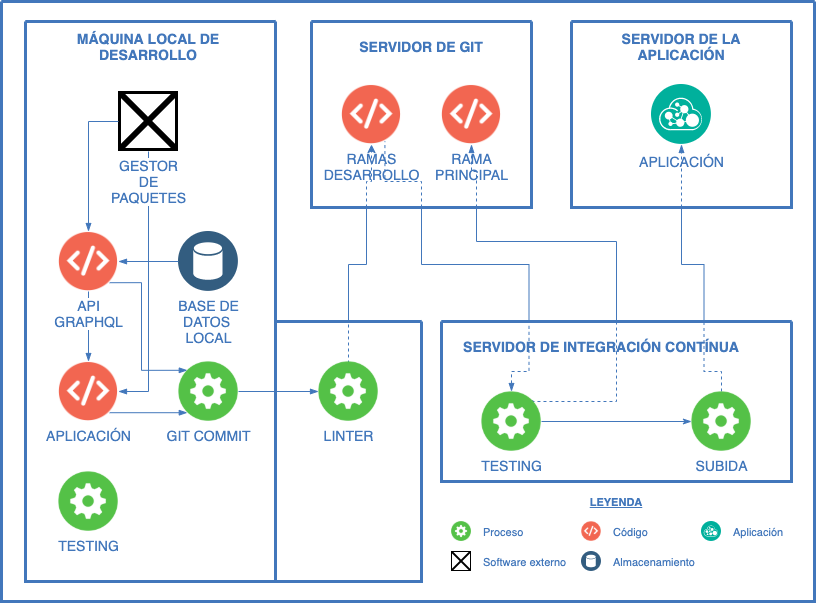
\includegraphics[width=\textwidth]{architecture.png}
  \caption{React Rocket Generator - Architecture}
  \label{fig:architecture}
\end{figure}

Una vez el código cumple los estándares propuestos por el linter y se sube a un repositorio mediante herramientas de control de versiones, se inicia un procedimiento automático descrito en el capítulo de \nameref{section:ci-cd-flow}. En este procedimiento, se utiliza una entidad llamada servidor de integración contínua, que es la responsable de que el flujo se cumpla. En esta entidad vuelven a estar visibles todas tecnologías de pruebas. La máquina de desarrollo tiene acceso a las tecnologías de pruebas como herramienta de desarrollo. Sin embargo, la máquina de integración contínua tiene acceso a estas tecnologías como parte del flujo de integración contínua, y si estás pruebas no son satisfechas, el código no se puede publicar ni en la rama principal ni en el servidor de la aplicación.

Por último, se encuentra el propio servidor de la aplicación, que contiene una versión comprimida del código, junto con la base de datos y la gls{api}. Este servidor es una entidad más compleja, dado que pueden ser varios servidores con un balanceador de carga. Es por eso que ese servidor no entra dentro del marco de desarrollo que se propone y se ha utilizado un icono distinto para representar toda esta complejidad. Cabe destacar que el servidor de integracón contínua y el de la aplicación pueden ser la misma máquina. Sin embargo, este no es el caso habitual y por eso se han marcado como entidades distintas.

Todo el marco está diseñado para que todo lo que hay en la máquina local sea automáticamente configurado mediante una serie de preguntas sencillas. Sin embargo, todo lo que corresponde a las otras máquinas pueden requerir configuración manual. El marco dispone de guías paso por paso para poder configurar todas las conexiones e integraciones descritas en la figura, así como los ficheros de configuración que alimentan el servidor de integración contínua. Todo esto queda explicado más adelante en detalle.

Cabe destacar que este trabajo parte de la premisa de que el marco es solo una propuesta inicial y que, tal y como se explica en el capítulo \nameref{chap:further-steps}, es una propuesta preparada para su expansión.


\label{chap:development}
\section{Funcionamiento general}
El marco de trabajo ha sido diseñado para ser lo más automático posible. Para realizar todas estas automatizaciones, NodeJS dispone de un gestor de paquetes (que se ha discutido en \nameref{section:packet-manager}). Este gestor se encarga de tener controladas todas las dependencias del proyecto. Para ello, utiliza un fichero mantenido por el equipo de desarrollo llamado package.json. Además, se genera otro fichero package-lock.json a partir del primero, que contiene las versiones exactas del proyecto.

Este fichero package.json tiene un valor muy especial para los desarrolladores de NodeJS porque además contiene otros campos con otras finalidades. Uno de los más importantes es el campo scripts, que permite poner a disposición mandatos de consola que realizan ciertas funcionalidades. El objeto scripts es un conjunto de pares clave-valor, donde la clave es el nombre del mandato y el valor es el comando bash que se va a ejecutar al utilizar ese mandato. Tenga en cuenta que este comando bash permite el uso de binarios que se encuentren dentro de las dependencias del proyecto, por lo que la potencia de estos scripts es infinita.

Con esta base, se ha decidido incluir en el proyecto uno de estos mandatos: el mandato setupº, que se encarga de montar el proyecto en función de las preferencias del usuario. Para ello, utiliza la librería Inquirer \cite{NPMLINQ}, que permite hacer una serie de preguntas al usuario mediante la consola. Una vez terminadas las preguntas, el mandato setup automáticamente elimina todos aquellos ficheros del repositorio que el usuario no va a utilizar (en función de sus preferencias), enlaza los que sí va a utilizar y deja preparados los scripts que el usuario pueda necesitar, de forma que el usuario pueda desde ese momento ponerse a trabajar. Se puede observar cómo se realizan las preguntas al usuario en las figuras \cref{fig:rocket-generator-1} y \cref{fig:rocket-generator-2}. En la figura \cref{fig:rocket-generator-3} se puede ver el final del script con todas las preguntas realizadas al usuario.

\begin{figure}
  \centering
  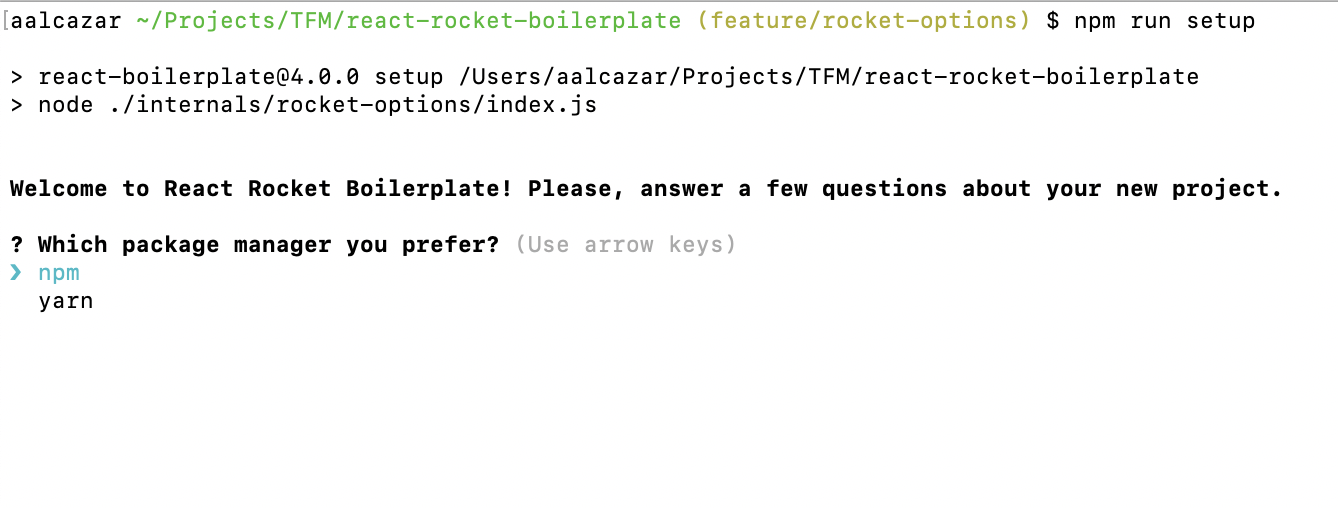
\includegraphics[width=\textwidth]{rocket-generator-1.png}
  \caption{React Rocket Generator - Asking about Package Manager}
  \label{fig:rocket-generator-1}
\end{figure}

\begin{figure}
  \centering
  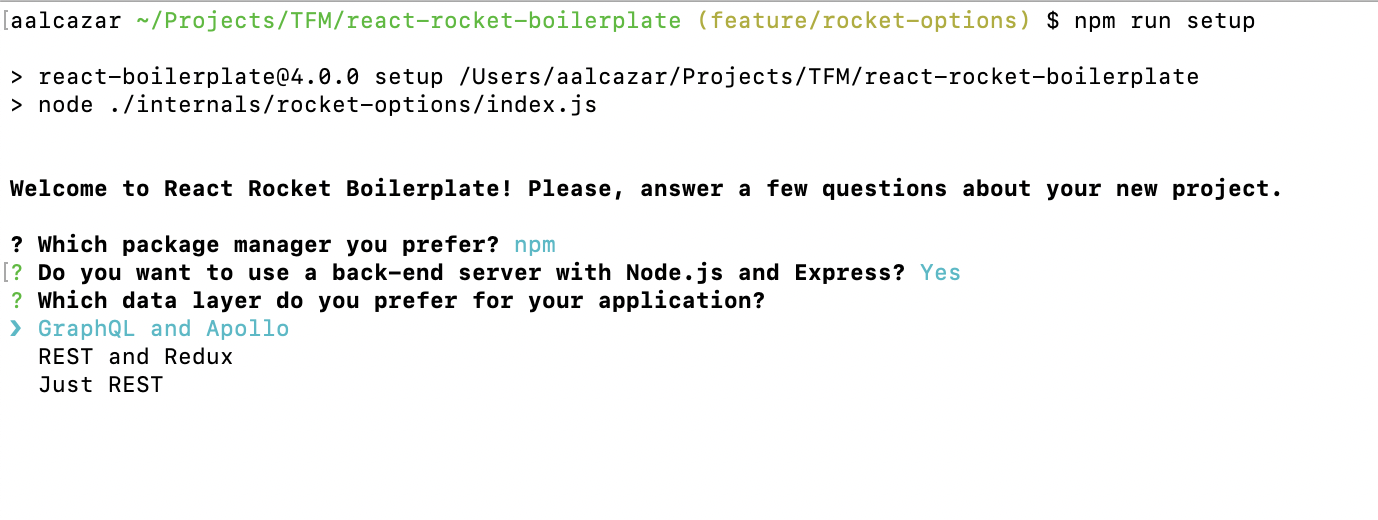
\includegraphics[width=\textwidth]{rocket-generator-2.png}
  \caption{React Rocket Generator - Asking about the API}
  \label{fig:rocket-generator-2}
\end{figure}

\begin{figure}
  \centering
  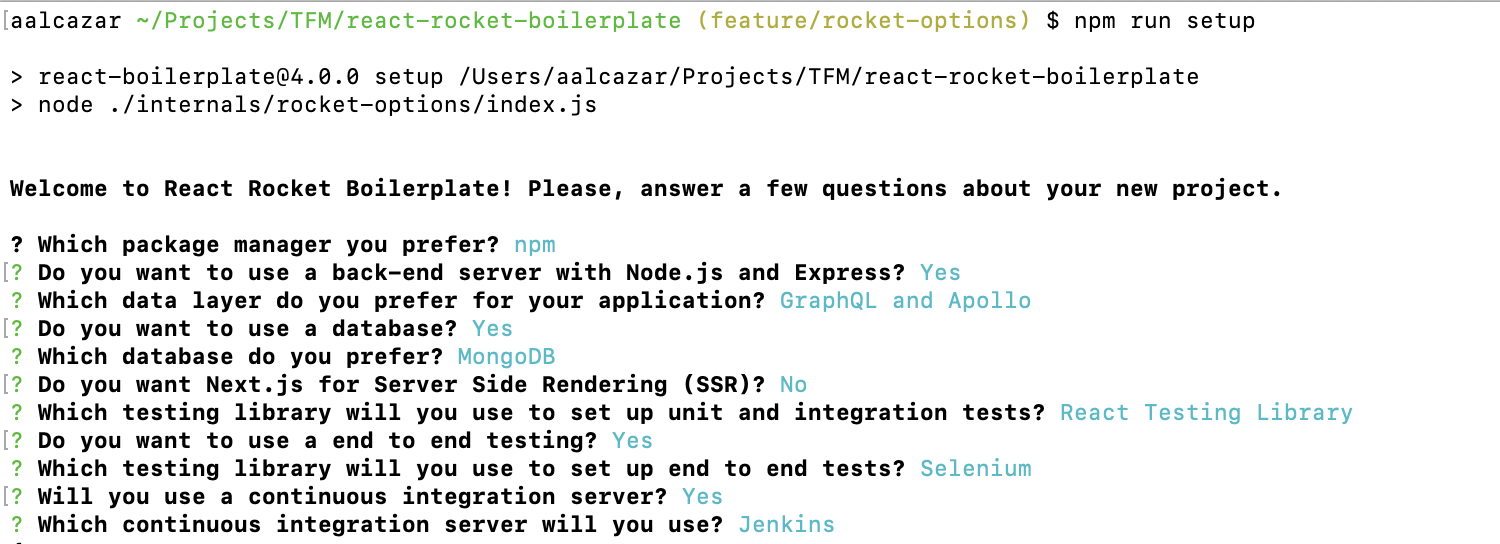
\includegraphics[width=\textwidth]{rocket-generator-3.png}
  \caption{React Rocket Generator - All questions together}
  \label{fig:rocket-generator-3}
\end{figure}

Cabe destacar que el proyecto se ha planteado como un proyecto abierto y la intención es ir incrementando el número de opciones de las que dispone el usuario para que el marco vaya siendo cada vez lo más completo posible. Cómo se puede ampliar el proyecto y cómo se ha planteado la ampliabilidad del proyecto se detalla más adelante en el apartado \nameref{chap:further-steps}.

El marco cuenta con un proyecto modelo para todas las opciones que introduzca el usuario. El proyecto modelo es una simple lista de tareas (ver lista de tareas vacía en la figura \cref{fig:todo-list-1}), en la cual el usuario puede añadir nuevas tareas (\cref{fig:todo-list-2}), marcar y desmarcar las tareas como hechas (\cref{fig:todo-list-3}), modificarlas y borrarlas. Este proyecto modelo ha sido realizado para todas las opciones de las que dispone el marco de trabajo: todos los tipos de base de datos incluídos en \nameref{section:database-manager} y todas las capas de datos incluídas en \nameref{section:data-layer}. Además, se ha cubierto el proyecto modelo con un 98\% de cobertura en pruebas para todos los tipos de proyecto modelo. Las pruebas se han realizado únicamente mediante Jest y React Testing Library (tal y como se comenta en \nameref{section:unit-testing}), pero entra dentro del ámbito del proyecto (tal y como se comenta más adelante en \nameref{chap:further-steps}) dar también soporte a Enzyme. Esto implicará repetir todas las baterías de pruebas para Enzyme.

\begin{figure}
  \centering
  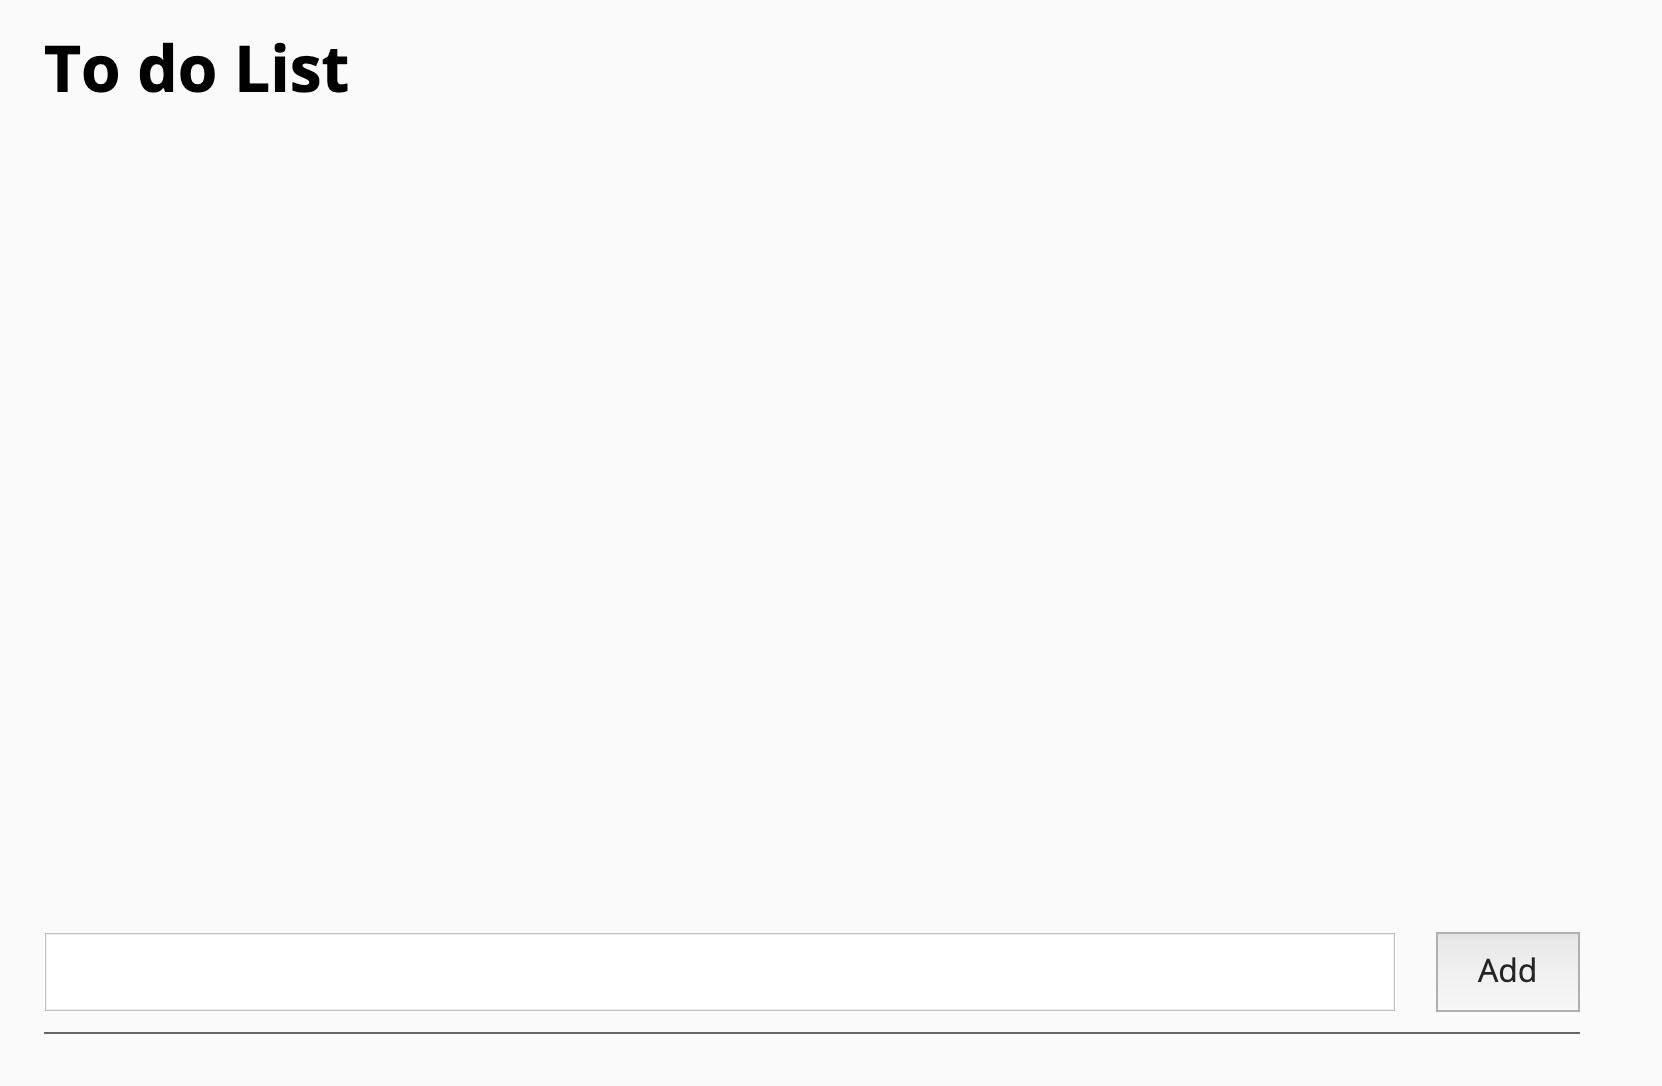
\includegraphics[width=\textwidth]{todo-list-1.png}
  \caption{React Rocket Todo List - Empty List}
  \label{fig:todo-list-1}
\end{figure}

\begin{figure}
  \centering
  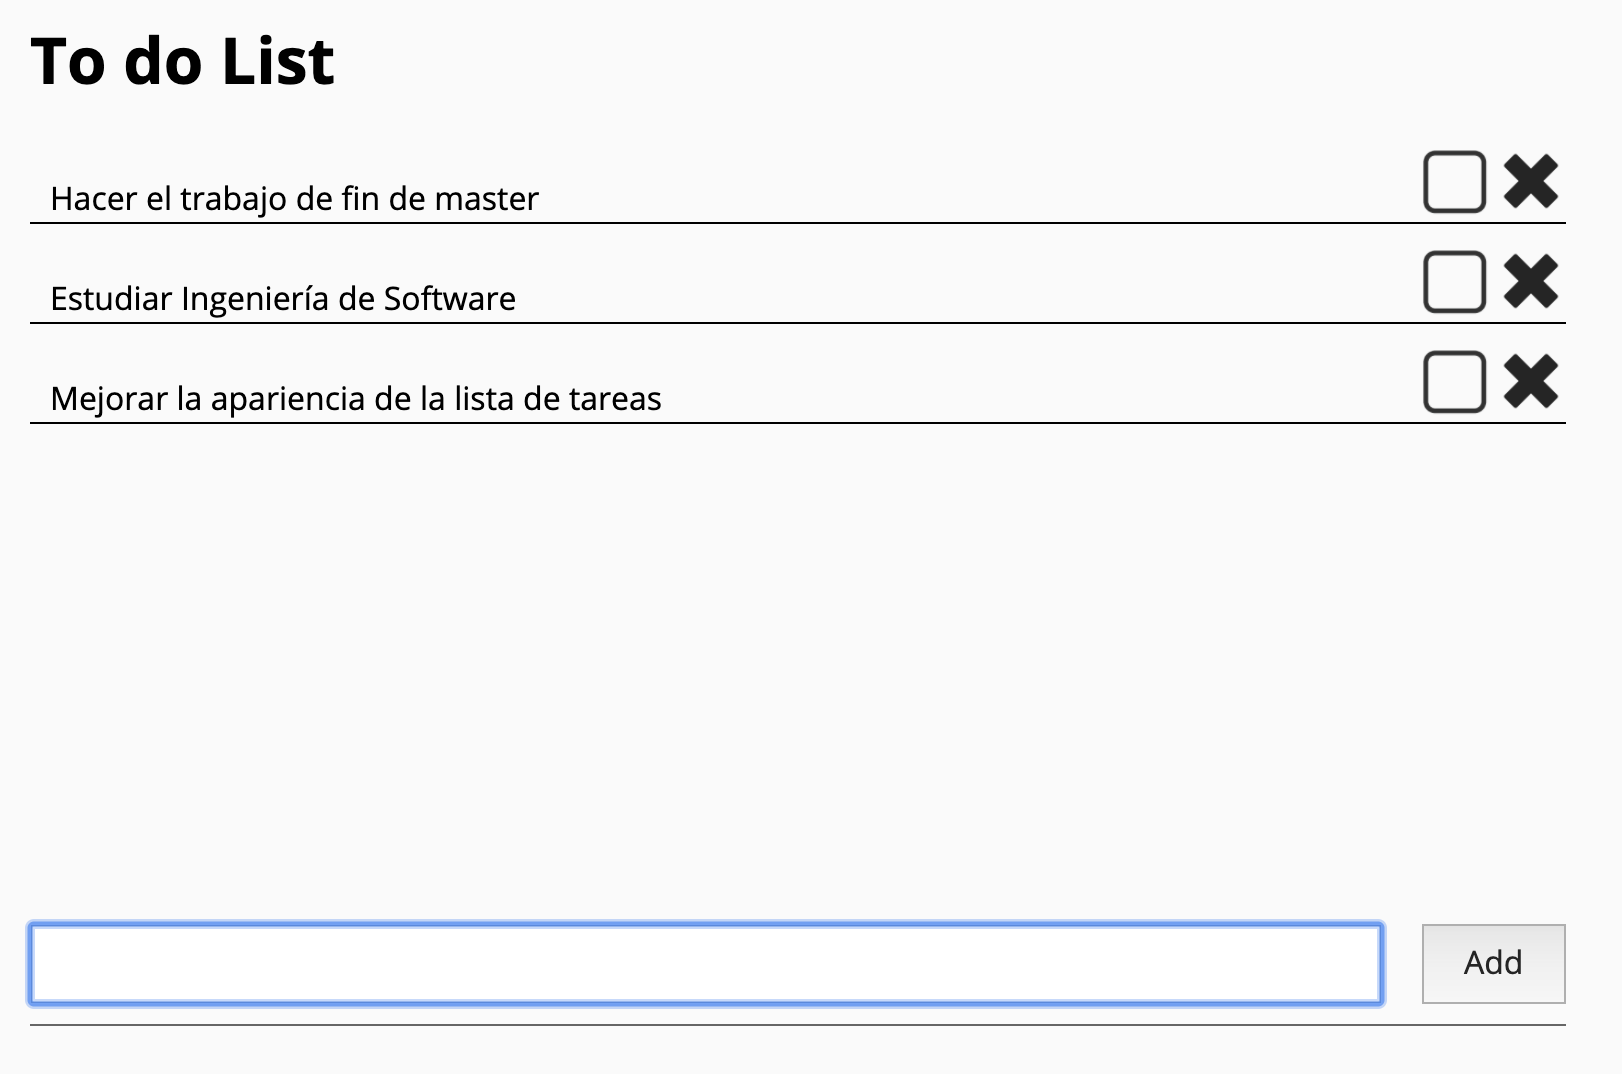
\includegraphics[width=\textwidth]{todo-list-2.png}
  \caption{React Rocket Todo List - Generated 3 items}
  \label{fig:todo-list-2}
\end{figure}

\begin{figure}
  \centering
  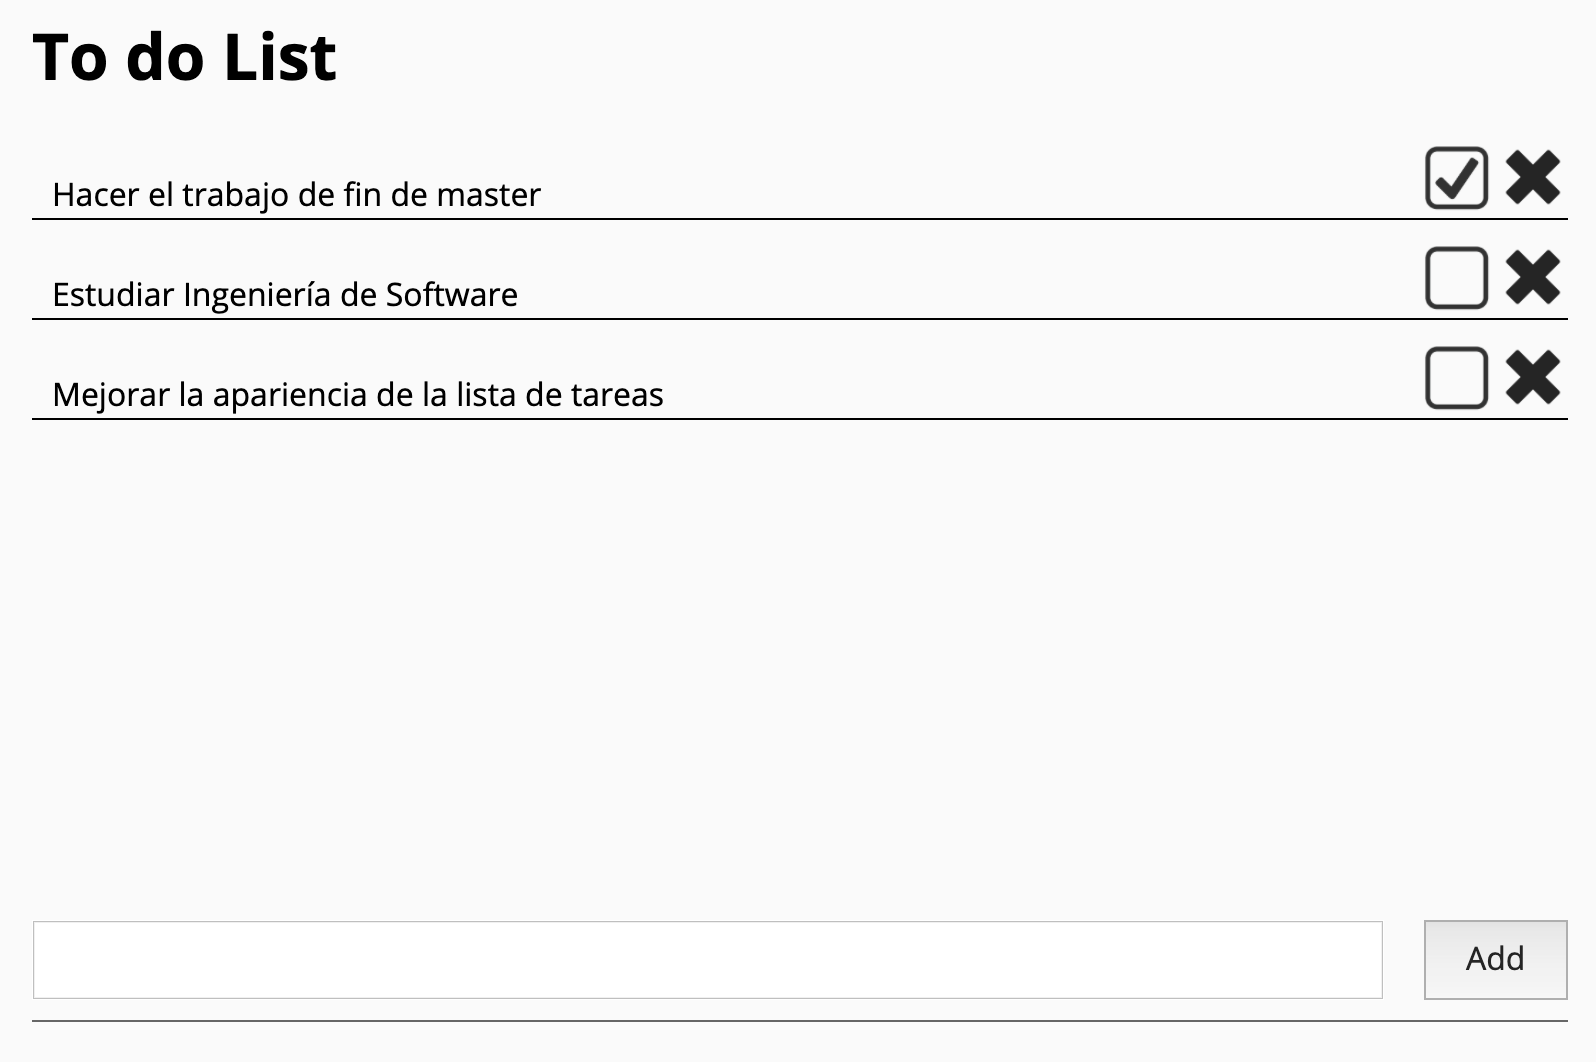
\includegraphics[width=\textwidth]{todo-list-3.png}
  \caption{React Rocket Todo List - Item marked as done}
  \label{fig:todo-list-3}
\end{figure}

Por último, el proyecto cuenta con integración continua integrada. Sin embargo, como esto depende de interacción explícita entre una cuenta registrada en un servidor de git (como Github) y una herramienta de desarrollo continuo (como Jenkins), ha sido imposible automatizar la instalación de la integración continua. Sin embargo, una vez están conectadas ambas herramientas mediante una cuenta con permisos suficientes, se ha logrado automatizar la tarea de integración continua mediante ficheros de configuración (tanto para Jenkins como para CircleCI), tal y como se especifica en el apartado \nameref{chap:ci-cd-detail}.

Con todo esto, el usuario del marco debería tener que hacer los siguientes pasos para poner en mancha un proyecto con este marco:
\begin{enumerate}
\item Clonar el repositorio del proyecto.
\item Ejecutar npm setup.
\item Responder a las preguntas sobre su proyecto. Una vez las termine, el proyecto podrá ser utilizado de forma local con la aplicación modelo descrita anteriormente.
\item Continuar con las instrucciones del README para poner en marcha la integración continua del proyecto.
\end{enumerate}

Como se puede observar, el proyecto es usable con muy poco esfuerzo. La parte más costosa es la de poner en marcha la integración contínua, que es definitivamente algo opcional. Aunque, por otro lado, utilizar este marco carece de sentido si no se pretende realizar un proyecto de calidad con pruebas automáticas e integración contínua.

A lo largo de este capítulo se irá mostrando el detalle completo de todas las partes involucradas en el marco.



\section{Detalle de la integración continua}
\label{chap:ci-cd-detail}
Para el desarollo de la integración continua y el despliegue continuo se han utilizado dos herramientas libres: Jenklins y CircleCI. El objetivo era minimizar el esfuerzo de configuración, pero esta tarea se dificulta sabiendo que, tal y como explica el diagrama de la figura \cref{fig:architecture}, puede haber un total de 4 máquinas interviniendo en el despliegue. Una de las cuales es el servidor de git y se asume que se está utilizando Github, así que se descarta. La máquina que se encarga del desarollo continuo es necesaria solo si se utiliza Jenkins o si se utiliza el plan de pago de CircleCI. Como se ha ido comentando a lo largo del trabajo, se descarta cualquier opción de pago, así que se va a asumir que si se utiliza Jenkins, se dispone de una máquina para el servidor de integración continua y si se utiliza CircleCI no.

Tanto jenkins como CircleCI disponen de la posibilidad de configurar el proyecto mediante un fichero de configuración que se incluye dentro del repositorio. Esto implica que el usuario no tendrá que preocuparse por casi nada de la configuración del proyecto. En el caso de Jenkins, este fichero se llama Jenkinsfile y utiliza la sintaxis Groovy y en el caso de CircleCI, este fichero se llama .circleci/config.yml y utiliza la sintaxis YAML. Sin embargo, ambas herramientas carecen de un método para generar automáticamente el proyecto, así que se requiere un mínimo trabajo manual para generar el proyecto y conectarlo al repositorio. En el caso de Jenkins, además, es necesario el plugin de Github y el plugin SSH Publisher para poder realizar una integración completa. Jenkins es ligeramente más complicado de montar porque requiere tener una máquina disponible para hacer de servidor. Sin embargo, su instalación es directa y se ejecuta únicamente mediante el mandato jenkins --daemon.

Respecto a la máquina que va a alojar el código, se espera que posea por lo menos los siguientes paquetes:
\begin{enumerate}
  \item git
  \item node y npm
  \item pm2: esta herramienta permite automatizar el despliegue en un solo fichero de configuración. El marco de trabajo asume que se utiliza pm2 para poder desplegar el código mediante un solo mandato.
  \item ssh: es necesario para poder comunicarse con la máquina.
  \item Visibilidad en la red: esto no es un paquete como tal, pero es un requisito indispensable. En el caso de Jenkins, la máquina objetivo debe estar dentro de la misma red (o ser la misma máquina) que la máquina que aloja Jenkins. En el caso de CircleCI, es imprescindible que la máquina tenga una dirección IP estática o tenga asociado un nombre de dominio a una IP Dinámica mediante \gls{ddns}. Además, deberá tener abiertos el puerto 80 y el 8080.
\end{enumerate}
Tal y como se comenta en \nameref{chap:further-steps}, se pretende dar soporte a Docker. Una vez se logre este hito, será indispensable que la máquina de la aplicación tenga instalado Docker. Para estos requisitos mínimos se ha elaborado un fichero de instalación que habrá que ejecutar una sola vez en la máquina que vaya a alojar el código, asumiendo que la máquina destino tiene acceso a apt. En caso de tener una distribución con otro servidor de paquetes, el usuario deberá buscar por su cuenta la forma de instalar los paquetes mencionados anteriormente. Dada una máquina con las características mencionadas, el fichero generado tanto para Jenkins como para CircleCI será capaz por sí mismo de ordenar a la herramienta en cuestión el despliegue automático en el servidor que vaya a alojar la aplicación.

Para simplificar el despliegue, se asume que la máquina que vaya a alojar la aplicación va a hacerlo utilizando el puerto 80 (o 443 en el caso de HTTPS) y que, la misma máquina va a utilizar el puerto 8080 para alojar la misma aplicación en preproducción. Además, se asume que la rama develop del servidor de git se conectará al servidor de preproducción y que la rama master se conectará al servidor de producción. Todo esto ya está contemplado en los ficheros de configuración tanto de Jenkins como de CircleCI.

Quiero aclarar que soy consciente de que esta es sin duda la parte más engorrosa del proyecto. Por su propia naturaleza, la variabilidad del entorno, la intervención de la red y el uso de herramientas muy gráficas como Jenkins y CircleCI, la cantidad de trabajo manual necesaria para poner en marcha el proyecto es mucho mayor de la que desearía. A lo largo del proyecto me he ido dando cuenta de la gran necesidad que hay de automatizar aun más todo este proceso y, por tanto, me he dado cuenta de que Docker debería haber sido parte del proyecto desde el principio. Sin embargo, mis recursos me han impedido añadirlo en esta primera fase y, por tanto, lo he dejado como máxima prioridad en el apartado de \nameref{chap:further-steps}. Docker no permitirá toda la automatización del sistema, pero sí permitirá una mejor integración con las herramientas mencionadas en este capítulo y reducirán mucho la carga de instalación de paquetes en la máquina que aloja la aplicación.





\chapter{Métricas del marco de trabajo}
\label{chap:metrics}

\section{Introducción}
Una vez ha sido construido el marco de trabajo, se ha realizado el proyecto "TODO List" con él, tal y como se explica en el apartado \nameref{chap:development}. Este proyecto se ha realizado de dos formas distintas: primero se ha realizado sin el marco de trabajo, y luego se ha repetido utilizando el nuevo marco.

El objetivo de este experimento es comprobar cuánto esfuerzo supone realizar un proyecto muy pequeño de forma que el resultado tenga calidad y sea escalable y, de ese modo, comprobar desde qué tipo de proyecto puede empezar a merecer la pena aplicar dicho esfuerzo.

La motivación original de este proyecto era conseguir reducir este esfuerzo inicial que supone realizar este trabajo mantenible y escalable. Lo ideal para este experimento habría sido que hubiese una población más grande y dividirla en tres grupos de desarrollo:

\begin{enumerate}
\item Los que hacen el proyecto sin aportar calidad.
\item Los que hacen el proyecto a partir del marco de trabajo y sin conocerlo previamente.
\item Los que hacen el proyecto con calidad, pero sin utilizar el marco de trabajo.
\end{enumerate}

De este modo, podríamos realizar un verdadero estudio estadísitico sobre lo que aporta de verdad el marco. Sin embargo, dados los recursos de este trabajo (tanto de tiempo como de capacidad de trabajo), tengo que reducir el experimento a un solo desarrollador (yo mismo) y prescindir del tercer grupo de trabajo. Además, una vez hecho el proyecto con marco de trabajo, al realizar el proyecto sin marco de trabajo ya habré pasado por un proceso previo de diseño y habré aprendido de mis errores en el desarrollo anterior. Por todo esto, la valided del experimento debe ser tomada con cuidado.

Aun así, se pueden sacar conclusiones de este experimento. El objetivo es tener una idea general de cuánto supone este esfuerzo, hacer una estimación de costes para una empresa pequeña y, de paso, comprobar si he echado de menos algo del marco de trabajo para poder tenerlo en consideración a futuro. Para poder sacar el máximo partido al experimento, en este apartado he realizado predicción sobre los resultados que esperaba y por qué antes de realizar dicho experimento. Una vez hecho el experimento, he complementado las predicciones con comentarios sobre las sorpresas que he recibido y las conclusiones que he sacado de los números obtenidos.


\section{Predicciones: resultados esperados}
Todas las estimaciones que se van a poder ver a continuación han sido realizadas bajo la asumción de que la persona que realiza las tareas domina las tecnologías que está utilizando. Para este proyecto se han estimado los siguientes tiempos sin utilizar el marco de trabajo ni aportando calidad al producto:

\begin{enumerate}
  \item Servidor: 3 horas
    \begin{enumerate}
      \item Montar el servidor (GraphQL y Express): 1 hora
      \item Añadir tarea: 0.5 hora
      \item Eliminar tarea: 0.5 hora
      \item Editar tarea: 0.5 hora
      \item Marcar tarea: 0.25 horas
      \item Obtener lista de tareas: 0.25 horas
    \end{enumerate}
  \item Cliente: 5.5 horas
    \begin{enumerate}
      \item Montar el cliente (Webpack): 2 horas
      \item Página de lista de tareas: 0.5 horas
      \item Componente de campo de texto: 0.5 horas
      \item Componente de botón de borrar tarea: 0.25 horas
      \item Componente de botón de editar tarea: 0.5 horas
      \item Componente de tarea: 0.25 horas
      \item Componente de caja de tareas: 0.25 horas
      \item Componente de botón de añadir tarea: 0.25 horas
      \item Integración con el servidor: 1 hora
    \end{enumerate}
  \item Subir a producción: 30 minutos
\end{enumerate}

En total, sin utilizar el marco de trabajo, se estima que se va a tardar 9 horas. En principio, en un día largo de trabajo podría abordarse el proyecto TODO List entero. El marco de trabajo se encargará de ahorrarnos las matesde montar el servidor, montar el cliente y la integración con el servidor. A cambio, nos exigirá un mínimo de cobertura en el código y nos facilitará engancharnos con un servidor de integración contínua. Por tanto, se espera que al utilizar el marco de trabajo el coste del proyecto sin preubas se reduzca en 3.5 horas aproximadamente. A cambio, se esperan los siguientes costes en pruebas:

\begin{enumerate}
  \item Pruebas unitarias en servidor: 5 horas
  \item Pruebas unitarias en cliente: 10 horas
  \item Pruebas de integración: 4 horas
  \item Pruebas funcionales: 6 horas
\end{enumerate}

Por tanto, se espera que el proyecto va a costar 32 horas utilizando el marco de trabajo para aportar calidad. Hay que tener en cuenta que, una vez terminado el proyecto con el marco de trabajo, se asume integración contínua y automática con Github, Jenkins, entorno de preproducción y producción. Cuanto más se modifique este proyecto a futuro, más rentable saldrá montar todo este entorno de calidad.

Además de los tiempos, es muy importante medir errores. En un proyecto tan pequeño, se esperan en total 10 errores máximo sin utilizar el marco de trabajo. En el proyecto con marco de trabajo no se espera ningún error.


\section{Resultados obtenidos}
Los resultados del experimento se han recogido en la tabla \cref{tab:results}. Como se puede observar, todas las tareas han implicado más esfuerzo debido a las pruebas unitarias que se han realizado haciendo el uso del marco. Sin embargo, la configuración inicial del proyecto mediante el marco de trabajo ha sido nula, tal y como estaba previsto. De esta tabla cabe destacar que el esfuerzo que nos ha ahorrado el marco de trabajo corresponde a las tareas de Montar el servidor y la integración con el servidor, que han sido un total de 3 horas.

Se han encontrado un total de 20 errores en la implementación sin marco, mientras que el marco nos ha evitado todos los errores. Estos errores han sido encontrados una vez he acabado los dos proyectos. He ido revisando todos los casos de prueba y realizándolos manualmente en el proyecto sin marco. El resultado ha sido que ha habido 20 problemas que, utilizando pruebas unitarias he identificado y resuelto con antelación, mientras que sin realizar estas pruebas se me han pasado por alto. El listado de errores concretos se puede encontrar en la tabla \cref{tab:errors}.

Una vez identificados los erroes, se ha dedicado esfuerzo a solucionarlos y se ha añadido una columna a la tabla \cref{tab:errors} con ese tiempo. El tiempo total ha sido de más de 4 horas. En la figura \cref{fig:results-comparison} se puede apreciar la diferencia del esfuerzo dedicado en el proyecto sin marco de trabajo y el proyecto con marco de trabajo, que casualmente ha sido de 4 horas.

En resumen, por un lado el proyecto sin marco de trabajo nos ha ahorrado 4 horas en total en desarrollo de pruebas unitarias. De las horas dedicadas, 3 han sido evitadas por el marco de trabajo. Es decir, que si hubiésemos realizado el proyecto sin código de calidad, pero utilizando el marco de trabajo, habríamos dedicado 8 horas en total. Por otro lado, se han producido 20 errores desarrollando sin pruebas automáticas, lo cual ha llevado 4 horas y 10 minutos solucionarlos.

% Please add the following required packages to your document preamble:
% \usepackage[table,xcdraw]{xcolor}
% If you use beamer only pass "xcolor=table" option, i.e. \documentclass[xcolor=table]{beamer}
\begin{table}[]
\centering
\caption{Tabla de resultados}
\label{tab:results}
\begin{adjustbox}{width=\columnwidth,center}
\begin{tabular}{llllll}
{\color[HTML]{000000} }                                                & {\color[HTML]{000000} }                         & \multicolumn{2}{l}{{\color[HTML]{000000} \textbf{Sin marco de trabajo}}}                              & \multicolumn{2}{l}{{\color[HTML]{000000} \textbf{Con marco de trabajo}}}                                                      \\
{\color[HTML]{000000} \textbf{Tarea}}                                  & {\color[HTML]{000000} \textbf{Tiempo estimado}} & {\color[HTML]{000000} \textbf{Tiempo empleado}} & {\color[HTML]{000000} \textbf{Errores encontrados}} & {\color[HTML]{000000} \textbf{Tiempo empleado (con marco)}} & {\color[HTML]{000000} \textbf{Errores encontrados (con marco)}} \\
{\color[HTML]{000000} \textbf{Montar el servidor (GraphQL y Express)}} & {\color[HTML]{000000} 1}                        & {\color[HTML]{000000} 1.5}                      & {\color[HTML]{000000} 2}                            & {\color[HTML]{000000} 0}                                    & {\color[HTML]{000000} 0}                                        \\
{\color[HTML]{000000} \textbf{Añadir tarea}}                           & {\color[HTML]{000000} 0.5}                      & {\color[HTML]{000000} 1}                        & {\color[HTML]{000000} 0}                            & {\color[HTML]{000000} 1.5}                                  & {\color[HTML]{000000} 0}                                        \\
{\color[HTML]{000000} \textbf{Eliminar tarea}}                         & {\color[HTML]{000000} 0.5}                      & {\color[HTML]{000000} 0.5}                      & {\color[HTML]{000000} 1}                            & {\color[HTML]{000000} 1}                                    & {\color[HTML]{000000} 0}                                        \\
{\color[HTML]{000000} \textbf{Editar tarea}}                           & {\color[HTML]{000000} 0.5}                      & {\color[HTML]{000000} 0.75}                     & {\color[HTML]{000000} 4}                            & {\color[HTML]{000000} 1.5}                                  & {\color[HTML]{000000} 0}                                        \\
{\color[HTML]{000000} \textbf{Marcar tarea}}                           & {\color[HTML]{000000} 0.25}                     & {\color[HTML]{000000} 0.25}                     & {\color[HTML]{000000} 1}                            & {\color[HTML]{000000} 0.75}                                 & {\color[HTML]{000000} 0}                                        \\
{\color[HTML]{000000} \textbf{Obtener lista de tareas}}                & {\color[HTML]{000000} 0.25}                     & {\color[HTML]{000000} 0.5}                      & {\color[HTML]{000000} 1}                            & {\color[HTML]{000000} 1}                                    & {\color[HTML]{000000} 0}                                        \\
{\color[HTML]{000000} }                                                & {\color[HTML]{000000} }                         & {\color[HTML]{000000} }                         & {\color[HTML]{000000} }                             & {\color[HTML]{000000} }                                     & {\color[HTML]{000000} }                                         \\
{\color[HTML]{000000} \textbf{Montar el cliente (Webpack)}}            & {\color[HTML]{000000} 2}                        & {\color[HTML]{000000} 2}                        & {\color[HTML]{000000} 0}                            & {\color[HTML]{000000} 0}                                    & {\color[HTML]{000000} 0}                                        \\
{\color[HTML]{000000} \textbf{Página de lista de tareas}}              & {\color[HTML]{000000} 0.5}                      & {\color[HTML]{000000} 0.5}                      & {\color[HTML]{000000} 0}                            & {\color[HTML]{000000} 2}                                    & {\color[HTML]{000000} 0}                                        \\
{\color[HTML]{000000} \textbf{Componente de campo de texto}}           & {\color[HTML]{000000} 0.5}                      & {\color[HTML]{000000} 0.25}                     & {\color[HTML]{000000} 1}                            & {\color[HTML]{000000} 0.5}                                  & {\color[HTML]{000000} 0}                                        \\
{\color[HTML]{000000} \textbf{Componente de botón de borrar tarea}}    & {\color[HTML]{000000} 0.25}                     & {\color[HTML]{000000} 0.25}                     & {\color[HTML]{000000} 1}                            & {\color[HTML]{000000} 0.75}                                 & {\color[HTML]{000000} 0}                                        \\
{\color[HTML]{000000} \textbf{Componente de botón de editar tarea}}    & {\color[HTML]{000000} 0.5}                      & {\color[HTML]{000000} 1}                        & {\color[HTML]{000000} 2}                            & {\color[HTML]{000000} 2}                                    & {\color[HTML]{000000} 0}                                        \\
{\color[HTML]{000000} \textbf{Componente de tarea}}                    & {\color[HTML]{000000} 0.25}                     & {\color[HTML]{000000} 0.5}                      & {\color[HTML]{000000} 4}                            & {\color[HTML]{000000} 1.25}                                 & {\color[HTML]{000000} 0}                                        \\
{\color[HTML]{000000} \textbf{Componente de caja de tareas}}           & {\color[HTML]{000000} 0.25}                     & {\color[HTML]{000000} 0.25}                     & {\color[HTML]{000000} 0}                            & {\color[HTML]{000000} 1.5}                                  & {\color[HTML]{000000} 0}                                        \\
{\color[HTML]{000000} \textbf{Componente de botón de añadir tarea}}    & {\color[HTML]{000000} 0.25}                     & {\color[HTML]{000000} 0.25}                     & {\color[HTML]{000000} 1}                            & {\color[HTML]{000000} 1.25}                                 & {\color[HTML]{000000} 0}                                        \\
{\color[HTML]{000000} \textbf{Integración con el servidor}}            & {\color[HTML]{000000} 1}                        & {\color[HTML]{000000} 1.5}                      & {\color[HTML]{000000} 2}                            & {\color[HTML]{000000} 0}                                    & {\color[HTML]{000000} 0}
\end{tabular}
\end{adjustbox}
\end{table}

\begin{table}[]
\centering
\caption{Tabla de errores}
\label{tab:errors}
\begin{adjustbox}{width=\columnwidth,center}
\begin{tabular}{rllr}
\multicolumn{1}{l}{\textbf{ID}} & \textbf{Tarea}                                  & \textbf{Descripción del error}                                                     & \multicolumn{1}{l}{\textbf{Tiempo de resolución (min)}} \\
1                               & \textbf{Montar el servidor (GraphQL y Express)} & El esquema GraphQL se lee con una codificación no soportada                        & 5                                                       \\
2                               & \textbf{Montar el servidor (GraphQL y Express)} & Error de CORS                                                                      & 5                                                       \\
3                               & \textbf{Eliminar tarea}                         & Eliminar tarea que no existe devuelve OK                                           & 15                                                      \\
4                               & \textbf{Editar tarea}                           & Editar tarea que no existe devuelve OK                                             & 15                                                      \\
5                               & \textbf{Editar tarea}                           & Editar una tarea marcada (toggled) quita la marca                                  & 5                                                       \\
6                               & \textbf{Editar tarea}                           & Editar una tarea sin texto devuelve OK                                             & 5                                                       \\
7                               & \textbf{Editar tarea}                           & Editar una tarea que tiene el texto repetido no funciona                           & 10                                                      \\
8                               & \textbf{Marcar tarea}                           & Marcar una tarea con el texto repetido a veces no funciona                         & 10                                                      \\
9                               & \textbf{Obtener lista de tareas}                & Si la lista se acaba de vacíar tras eliminar tarea, devuelve error                 & 30                                                      \\
10                              & \textbf{Componente de campo de texto}           & Si la API devuelve error, muestra ese error en el campo de texto                   & 5                                                       \\
11                              & \textbf{Componente de botón de borrar tarea}    & Borrar una tarea recién reordenada borra una tarea distinta                        & 10                                                      \\
12                              & \textbf{Componente de botón de editar tarea}    & Editar una tarea recién reordenada edita una tarea distinta                        & 10                                                      \\
13                              & \textbf{Componente de botón de editar tarea}    & Editar una tarea sin cambiar el texto envía un vacío a la API                      & 5                                                       \\
14                              & \textbf{Componente de tarea}                    & Reordenar una tarea marcada la desmarca                                            & 15                                                      \\
15                              & \textbf{Componente de tarea}                    & Editar una tarea la cambia de orden                                                & 10                                                      \\
16                              & \textbf{Componente de tarea}                    & Editar una tarea y no ponerle texto genera un error en consola                     & 5                                                       \\
17                              & \textbf{Componente de tarea}                    & Marcar y desmarcar una tarea rápidamente la hace desaparecer                       & 45                                                      \\
18                              & \textbf{Componente de botón de añadir tarea}    & Añadir tarea sin escribir nada en el campo de texto envía una petición al servidor & 5                                                       \\
19                              & \textbf{Integración con el servidor}            & Inconsistencia de la cache de Apollo con respecto a los datos del servidor         & 30                                                      \\
20                              & \textbf{Integración con el servidor}            & Error con el tamaño máximo de carga                                                & 10                                                      \\
\multicolumn{3}{l}{\textbf{Tiempo total (min)}}                                                                                                                        & 250                                                     \\
\multicolumn{3}{l}{\textbf{Tiempo total (horas)}}                                                                                                                      & 4.166666667
\end{tabular}
\end{adjustbox}
\end{table}

\begin{figure}
  \centering
  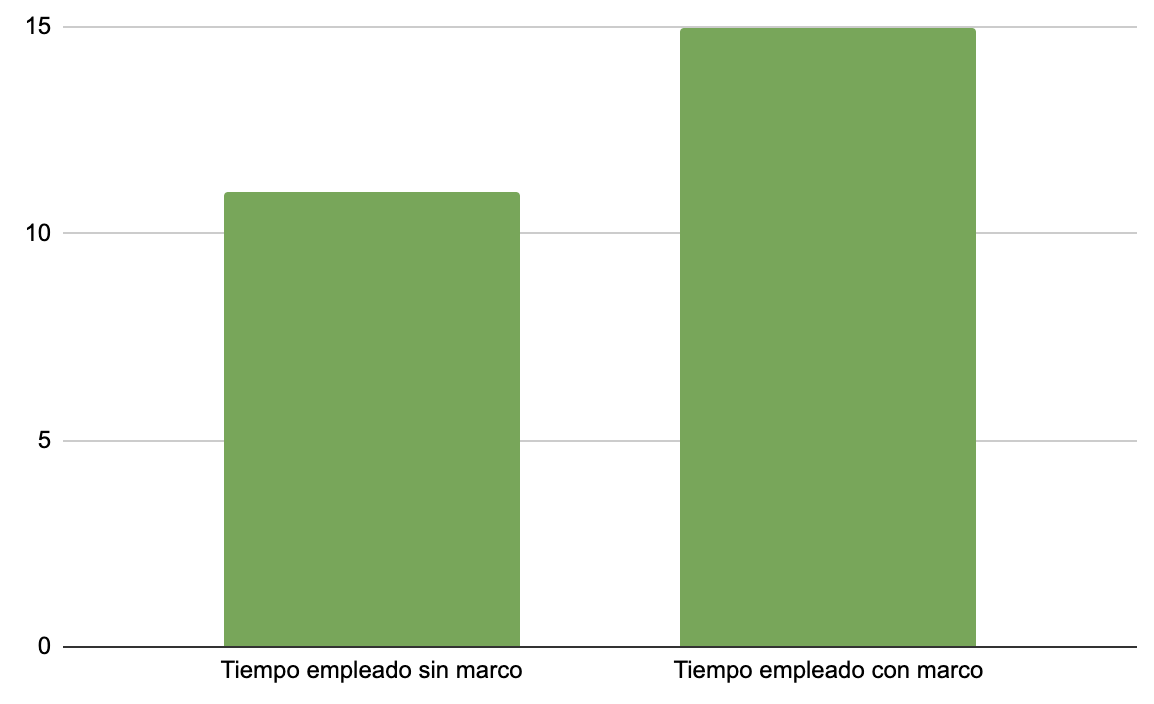
\includegraphics[width=\textwidth]{results-comparison.png}
  \caption{Comparación entre el tiempo dedicado con y sin pruebas}
  \label{fig:results-comparison}
\end{figure}



\section{Conclusiones}
Lo primero que me ha sorprendido al ver los números finales es que se ha amortizado el tiempo dedicado a hacer las pruebas unitarias. He experimentado esta amortización en proyectos más grandes, pero no me esperaba que en un proyecto de esta escala las horas dedicadas a solucionar errores fuesen a ser mayores a las horas dedicadas a realizar pruebas untiarias. Hay que tener en cuenta que, tal y como se comenta en la introducción de \nameref{chap:metrics}, este experimento ha sido muy limitado y hay que coger con pinzas estos resultados, pero ya nos hacemos a la idea que en ocasiones e incluso para proyectos pequeños, hacer pruebas unitarias puede salir rentable.

Para hacer justicia a la verdad, el tiempo total dedicado a realizar las pruebas automáticas ha sido de 7 horas. Sin embargo, con el descuento que nos hace el marco de trabajo con toda la configuración del entorno ha salido rentable. En proyectos más grandes esto es mucho más difícil de medir, pero los errores tienden a escalar en profundidad y suelen ser más difíciles de depurar. Además, a esto habría que sumar pruebas de integración y funcionales, que no se han realizado por la simplicidad del proyecto.

Otro dato que me ha sorprendido es la cantidad de errores que se han producido. 20 errores en un código de aproximadamente 5600 líneas de código implica a un error cada 280 líneas de código. Es de esperar que a este ritmo, si se comienza una prueba de concepto sin código de calidad, a la hora de realizar el escalado cualquiera de estos muchos errores va a pasar factura más adelante. Los errores predecidos eran 10, así que aunque el proyecto sea bien conocido y de dimensiones limitadas, los errores están a la orden del día. En un proyecto de prueba, podríamos llegar a esperar un error cada 150 líneas de código. Esto hace mucho más acuciante la necesidad de utilizar código de calidad.

El tiempo que nos ha ahorrado el marco de trabajo ha sido de 3 horas, pero no es un dato muy representativo dado que gran parte de la potencia del marco no se ha utilizado. No se ha utilizado ningún servidor de integración contínua ni se ha desplegado el proyecto en ningún sitio, así que esas 3 horas de ahorro se pueden considerar como el mínimo. Además, estas 3 horas son lo que he tardado yo en configurar el proyecto, que soy la misma persona que ha realizado el marco de trabajo y, por tanto, se ha estudiado numerosas posibles configuraciones y comprende las interacciones de Express, Webpack, React y GraphQL con bastante profundidad. Una persona que está explorando un campo nuevo puede dedicar incluso una semana entera a configurar el proyecto, así que este ahorro no ha quedado bien reflejado en el experimento.

Así que, como conclusión final del experimento, este marco de trabajo ha sido muy positivo incluso para proyectos pequeños porque alivia la carga de configuración del proyecto, tal y como se pretendía, preparando el entorno para la realización de pruebas automáticas y evitando esos 20 errores que podrían costar una fortuna si se encuentran una vez el proyecto ha escalado y está en producción.

Aun así, como el experimento ha sido limitado queda por comprobar si realmente en un caso de uso real este marco de trabajo es de utilidad. Y la única forma de comprobarlo es con tiempo y esperando la retroalimentación de los usuarios del marco. La apuesta, sin embargo, es que este marco va a ser de gran utilidad siempre y cuando el compromiso de realizar código de calidad sea real.



\chapter{Discusión de los objetivos}
TODO


\chapter{Conclusiones del proyecto}
Durante este proyecto se ha investigado una numerosa cantidad de tecnologías y se han recogido las más frecuentes en el ámbito del desarrollo web. Se ha analizado cuáles combinan bien entre ellas, se ha creado un entorno que facilita la configuración rápida del proyecto y se ha generado un proyecto de pruebas para cada tecnología seleccionada.

El objetivo era facilitar la producción de pruebas de concepto de calidad, de modo que pudiesen escalar de forma rápida y sin errores. Para eso hace falta seguir una serie de buenas prácticas y construir una buena batería de pruebas desde el primer minuto.

Para demostrar que este objetivo se cumple, se ha realizado un experimento sencillo: se ha creado un proyecto en una versión sin marco y otra versión con marco. Se han comparado, y ha resultado que la versión con marco, para este caso particular, nos ha ahorrado 20 errores en tan solo 4 horas más de codificación. Si consideramos el tiempo de resolver esos errores, el marco nos ha permitido dedicar el mismo tiempo que si lo hubiésemos hecho sin marco, pero teniendo la batería de pruebas generada y, por tanto, previniendo futuros errores que pudiesen surgir con la evolución del proyecto.

Después de todo el esfuerzo y viéndolo con perspectiva, he llegado a la conclusión de que la cantidad de tecnologías soportadas no es suficiente para cubrir la mayoría de necesidades del mundo del desarrollo web y, cuantas más tecnologías cubra el marco, más rápida va a ser la configuración de las pruebas de concepto y más útil va a ser el marco. Así que, para cubrir un mayor número de tecnologías, hace falta abrir el código y trabajar más en el producto.

Aun así, la experiencia de utilizar el marco de trabajo tal y como está ahora ha sido muy gratificante. Tener un esqueleto de proyecto que asegura calidad tan solo respondiendo unas cuantas preguntas, que ese esqueleto sea flexible a las tecnologías implicadas y que incluya ficheros de configuración para integración continua es exactamente lo que personalmente necesito para motivarme a que mis pruebas de concepto tengan calidad desde el primer momento.

Así que espero ser capaz de transmitir esta experiencia a otros usuarios y que poco a poco este marco se vaya transformando en una necesidad para todo aquél que desee empezar un proyecto de cero. También espero que el marco sea semilla de proyectos de calidad y, de este modo, animar al resto de desarrolladores a comenzar con buen pie cada idea que tengan por pequeña que sea.




\chapter{Futuras líneas de trabajo}
\label{chap:further-steps}

\section{Abrir el código}
El alcance del trabajo está limitado a las horas impuestas y, dadas las circunstancias, se ha decidido acotar a unas pocas tecnologías elegidas generalmente mediante el criterio de la popularidad, de forma que este marco pueda ser útil al mayor número posible de desarrolladores. El código ya ha sido escrito con eso en mente y, por tanto, se ha preparado el terreno para dar un paso evidente en el ciclo: publicar el código como abierto.

Esto tiene las siguientes ventajas:
\begin{enumerate}
  \item El código es revisado por numerosos desarrolladores, dando distintos puntos de vista y aportando diversidad.
  \item El código se produce a más velocidad y los errores se resuelven más rápido, sin coste alguno.
  \item El proyecto se puede reutilizar y se pueden generar otros marcos y otras ideas.
  \item El marco se puede ampliar a más tecnologías porque más usuarios lo van a dar forma en función de sus necesidades.
\end{enumerate}

Sin embargo, el código abierto no es un paso pequeño. Tal y como constata el estándar de código abierto \cite{OPENSRC}, tiene una serie de responsabilidades para el dueño originario del código para que pueda funcionar, que en este marco son necesarias. Estas responsabilidades son, en general, buenas prácticas para cualquier código, pero en este marco en particular son unos requisitos indispensables a ser abordados antes de poder publicar el código como abierto:
\begin{enumerate}
  \item Todo el código debe estar revisado y comentado en función de una guía de buenas prácticas. La dificultad de esta tarea se va a reducir porque se utilizó Linter desde el primer momento, pero aun así una revisión de calidad es necesaria.
  \item El marco debe estar documentado en su totalidad. En el estado actual del proyecto, toda la documentación se refiere a como construir un proyecto a partir del marco, pero el marco en sí debe ser documentado mediante el punto de vista del editor del marco. Esto implica documentar las tareas automáticas y una guía de amplicación de las tencologías disponibles. Para hacer estas guías, es razonable realizar una amplicación por mí mismo para comprobar que todo funciona como se había planteado.
  \item Elaborar los documentos requeridos para el código abierto: Licencia, README, Guía de contribución y Código de conducta. El README ya está generado, pero requerirá una revisión y quizá nuevos apartados para la instalación desde un punto de vista de contribución.
\end{enumerate}

En el momento en el que el código se transforme en código abierto, se habrá cumplido el verdadero propósito del proyecto y se considerará iniciada la primera versión oficial del producto. Por tanto, el código ha de estar totalmente completo desde todos los puntos de vista posibles. El estado actual del producto es que es completo y listo para ser utilizado como marco, como semilla de otros proyectos. Pero faltan una serie de pasos para poder ser ampliado libremente y esto requiere planificación y revisión, así que esto será, en definitiva, el próximo paso más inmediato.


\section{Ampliabilidad del código}
Uno de los pasos fundamentales para poder publicar el código abierto es que sea ampliable. Como la idea es que la tarea de ampliar el marco se va a repetir en numerosas ocasiones, se ha planteado la opción de automatizarla en la medida de lo posible. Por tanto, teniendo en cuenta el futuro, he diseñado el proceso de ampliación y las tareas que van a facilitar la tarea. Supongamos que un usuario desea ampliar el código con una tecnología particular -digamos que por ejemplo desea añadir Redis como base de datos- así que se clona el respositorio y se instala las dependencias. Lo ideal sería que ese usuario ejecutase una tarea framework:expand y que, mediante el mismo sistema que utiliza el marco para comenzar un proyecto, le hiciese unas preguntas sobre su ampliación.

Estas preguntas buscarán obtener la siguiente información:
\begin{enumerate}
  \item Conocer el nombre de la tecnología a implementar. En este caso Redis
  \item Conocer el tipo de tecnología a implementar. En este caso Base de datos.
  \item Conocer qué ficheros implicados ha de poseer el marco, que deberá eliminar si el usuario no elige la tecnología.
  \item Conocer qué tarea del package.json deberá aplicar al instalar el marco en caso de necesitarla. En este caso particular, el usuario puede querer producir una instancia de la base de datos en su instalación.
  \item Conocer las opciones con las que se puede utilizar esta tecnología en el marco. Estas opciones serán luego ofrecidas al usuario final durante la fase de preguntas si elige utilizar esta nueva tecnología, Redis, y el resultado de la selección se le pasará a esa tarea de inicialización del package.json para que el usuario desarrollador pueda trabajar con ellas.
\end{enumerate}

Con toda esta información, el marco será capaz de mantener un registro de los ficheros asociados, podrá pasar pruebas automáticas con distintas configuraciones y podrá actualizar una documentación online sobre las tecnologías disponibles. Todas estas tareas quedan a responsabilidad del propio marco y no del usuario.

Como la intención no es restringir, si no ayudar, esta tarea debe ser una mera inicialización de la nueva tecnología, pero todo debe poder ser editado al vuelo. Por tanto, esta tarea no hará más que generar información en una serie de ficheros que podrán ser editados. Estos ficheros serán la clave de la ampliabilidad, dado que permiten documentar de forma automática el marco y, a la vez, automatizar todas las tareas de instalación.

Por otro lado, el usuario quedará responsable de cumplir los requisitos de cobertura para su tecnología en la aplicación de pruebas "Lista de tareas", generar las tareas automáticas de instalación y mantener los ficheros mencionados en el párrafo anterior. Aun así, una vez el código pasa esas pruebas y está listo para ser subido, requerirá una revisión manual por parte de los encargados del mantenimiento del código, que será un equipo compuesto por personas de confianza que hayan contribuido al código. En la imagen inicial, estas ampliaciones solo requerirán de mi revisión manual.

La idea es que, de forma inicial, la ampliación del código sea lo más sencilla y automática posible. Y que, poco a poco, con contribuciones de distintos desarrolladores, el sistema se vaya cerrando más y quede totalmente automatizado. Todavía no se ha diseñado exactamente qué ficheros van a participar y qué estructura van a tener, pero esto será uno de los pasos requeridos antes de poder publicar el código como abierto.


\section{Próximas tecnologías a abordar}
Una vez se haya abierto el código, mi tarea con el marco no ha concluido. Además de las revisiones que tendré que hacer y de la resolución de errores que vayan surgiendo, quedará a mi responsabilidad contribuir a la ampliación del marco por mí mismo. De este modo, podré probar si todo lo que he diseñado para la ampliación funciona bien y tiene sentido. Además, se publicará una serie de tecnologías que han sido contempladas en la fase de investigación pero no han podido ser incluídas en el marco original por falta de tiempo y alcance en el trabajo.

Queda a mi responsabilidad el ir añadiendo poco a poco estas tecnologías a menos que algún contribuyente decida abordar alguna por sí mismo. Esta lista ya ha sido pensada en la fase de investigación, pero quedará expuesta a posibles cambios en función de la demanda en el apartado Issues de Github, que tendrá una etiqueta disponible para pedir ampliaciones de tecnologías. Mi tarea consistirá en ir añadiendo las más populares, independientemente de la lista que voy a añadir a continuación. Sin embargo, por el momento y mientras el marco no tenga suficiente público, se irán abordando en el orden en que considero más necesario a raíz de este trabajo.

Es evidente que la dirección concreta que va a tomar el marco depende en su totalidad de su popularidad. En el desafortunado caso de que este marco no logre darse a conocer o no logre ser de suficiente utilidad, el marco quedará completo cuando las tecnologías de la lista hayan sido añadidas. En caso de que el marco adquiera uso y la demanda aumente, es probable que la lista cambie de forma en función de esta demanda.

Así que, como último apartado de los últimos pasos, será añadir las siguientes tecnologías en el orden propuesto:
\begin{enumerate}
  \item Docker: es imprescindible que el marco de soporte a contenedores Docker y, por tanto, esta será la máxima prioridad. Esto además tiene grandes repercusiones sobre la integración continua y facilita mucho la tarea del despliegue y el escalado.
  \item Enzyme: numerosos desarrolladores están trabajando con Enzyme en lugar de React Testing Library. Me parece requisito indispensable que acabe entrando dentro del marco como máxima prioridad.
  \item Redis: una base de datos libre que se utiliza en numerosos proyectos.
  \item Vue
  \item AngularJS
  \item Go: esta idea todavía no la tengo clara, dado que todo el marco está en NodeJS. Sin embargo, sería adecuado si otros lenguajes pudiesen ser utilizados en el lado de servidor. Go parece ser la alternativa a NodeJS que más está entrando en el mercado. De todos modos, esta opción queda pendiente a ser evaluada cuando llegue el momento.
  \item Kubernetes y, en el futuro, otras herramientas de escalado flexible: el objetivo es que el usuario comience su proyecto de forma rápida pero tenga acceso a todas las herramientas de escalado de forma relativamente sencilla. El escalado nunca es una tarea fácil, pero el mundo dispone de herramientas como Kubernetes que, una vez se ha integrado el proyecto con Docker, es más asequible que nuestro proyecto aumente de tamaño sin miedo a perder el control. Kubernetes se encarga de gestionar los distintos nodos que interactuan en nuestro proyecto, generando o eliminando instancias en función de la demanda. Por tanto, para que el marco de trabajo se pueda utilizar de forma profesional, debe haber un soporte adecuado para este tipo de herramientas.
\end{enumerate}


\printbibliography

Todos los enlaces han sido comprobados el 22 de Febrero de 2020.
% Todos los enlaces han sido comprobados el May 19, 2020.

% \appendix
% % !TeX root = main-english.tex
% !TeX spellcheck = en-US
% !TeX encoding = utf8
% -*- coding:utf-8 mod:LaTeX -*-

%This smart spell only works if no changes have been made to the chapter 
%using the options proposed in preambel/chapterheads.tex.
\setchapterpreamble[u]{%
  \dictum[Albert Einstein]{We cannot solve our problems with the same level of thinking that created them}
}
\chapter{LaTeX Hints}
\label{chap:latexhints}

One sentence per line.
This rule is important for the usage of version control systems.
A new line is generated with a blank line.
As you would do in Word:
New paragraphs are generated by pressing enter.
In LaTeX, this does not lead to a new paragraph as LaTeX joins subsequent lines.
In case you want a new paragraph, just press enter twice (!).
This leads to an empty line.
In word, there is the functionality to press shift and enter.
This leads to a hard line break.
The text starts at the beginning of a new line.
In LaTeX, you can do that by using two backslashes (\textbackslash\textbackslash).
This is rarely used.

Please do \textit{not} use two backslahes for new paragraphs.
For instance, this sentence belongs to the same paragraph, whereas the last one started a new one.
A long motivation for that is provided at \url{http://loopspace.mathforge.org/HowDidIDoThat/TeX/VCS/#section.3}.

One can write \emph{emphasized text (rendered in italics)} and \textbf{bold text}.

\section{File Encoding and Support of Umlauts}
\label{sec:firstsectioninlatexhints}
The template offers foll UTF-8 support.
All recent editors should not have issues with that.

\section{Citations}


References are set by means of \texttt{\textbackslash cite[key]}.

\begin{filecontents*}{\democodefile}
Example: \cite{WSPA} or by author input: \citet{WSPA}.
\end{filecontents*}
\PrintDemo{style=parallel}

The following sentence demonstrates
\begin{inparaenum}[1.]
  \item the capitalization of author names at the beginning of the sentence,
  \item the correct citation using author names and the reference,
  \item that the author names are a hyperlink to the bibliography and that
  \item the bibliography contains the name prefix \qq{van der} of \qq{Wil M.\,P.\ van der Aalst}.
\end{inparaenum}

\begin{filecontents*}{\democodefile}
\Citet{RVvdA2016} present a study on the effectiveness of workflow management systems.
\end{filecontents*}
\PrintDemo{style=parallel}

The following sentence demonstrates that you can overwrite the text part of the generated label using \texttt{label} in a bibliopgrahie"=entry, but the year and the uniqueness is still generated by biber.

\begin{filecontents*}{\democodefile}
The workflow engine Apache ODE \cite{ApacheODE} executes \BPEL processes reliably.
\end{filecontents*}
\PrintDemo{style=parallel}

\begin{filecontents*}{\democodefile}
Words are best enclosed using \texttt{\textbackslash qq\{..\}}, then the correct quotes are used.
\end{filecontents*}
\PrintDemo{style=parallel}

When creating the Bibtex file it is recommended to make sure that the DOI is listed.

\section{Formulas and Equations}
\label{sec:mf}

\begin{filecontents*}{\democodefile}
Equations $f(x)=x$ inside the text can be provided.
\end{filecontents*}
\PrintDemo{style=parallel}

A list with all available mathematical symbols is provided at \url{http://texdoc.net/pkg/symbols-a4}.

\begin{filecontents*}{\democodefile}
As example the set of natural numbers is given by $\mathbb{N}$.
\end{filecontents*}
\PrintDemo{style=parallel}

For the documentation of editing mathematical formulas read the package documentation of \texttt{amsmath}\footnote{\url{http://texdoc.net/pkg/amsmath}}.

Equation~\ref{eq:test} is numbered and can be referenced in the text:
\begin{filecontents*}{\democodefile}
\begin{align}
  \label{eq:test}
  x = y
\end{align}
\end{filecontents*}
\PrintDemo{style=parallel}

Following equation is not numbered because of using \texttt{\textbackslash align*} as environment.
\begin{filecontents*}{\democodefile}
\begin{align*}
  x = y
\end{align*}
\end{filecontents*}
\PrintDemo{style=parallel}

The template offers \verb+\abs+ to enable the bars scaling well at the absolute value:

\begin{filecontents*}{\democodefile}
$\abs{X}$.
\end{filecontents*}
\PrintDemo{style=parallel}

More details about mathematical environments provides the documentation available at \url{http://www.ctan.org/tex-archive/help/Catalogue/entries/voss-mathmode.html}.


%%%%%%%%%%%%%%%%%%%%%%%%%%%%%%%%%%%%%%%%%%%%%%%%%%%%%%%%%%%%%%%%%%%%%%%%%%%%%%
\section{Sourcecode}
%%%%%%%%%%%%%%%%%%%%%%%%%%%%%%%%%%%%%%%%%%%%%%%%%%%%%%%%%%%%%%%%%%%%%%%%%%%%%%
\Cref{lst:ListingANDlstlisting} shows how to emmbed source code.
With \texttt{\textbackslash lstinputlisting} the source code can be loaded directly from files.

%Listing-Umgebung wurde durch \newfloat{Listing} definiert
\begin{Listing}
  \begin{lstlisting}
<listing name="second sample">
  <content>not interesting</content>
</listing>
\end{lstlisting}
  \caption{The code is separated by two horizontal lines in the listings environment.}
  \label{lst:ListingANDlstlisting}
\end{Listing}

\begin{filecontents*}{\democodefile}
Source code is also available in the text \lstinline|<listing />|.
\end{filecontents*}
\PrintDemo{style=parallel}


%%%%%%%%%%%%%%%%%%%%%%%%%%%%%%%%%%%%%%%%%%%%%%%%%%%%%%%%%%%%%%%%%%%%%%%%%%%%%%
\section{Pseudocode}
%%%%%%%%%%%%%%%%%%%%%%%%%%%%%%%%%%%%%%%%%%%%%%%%%%%%%%%%%%%%%%%%%%%%%%%%%%%%%%
\Cref{alg:sample} shows a sample algorithm.
\begin{Algorithmus} %Use the environment only if you want to place the algorithm similar to graphics from TeX
  \caption{Sample algorithm}
  \label{alg:sample}
  \begin{algorithmic}
\Procedure{Sample}{$a$,$v_e$}
\State $\mathsf{parentHandled} \gets (a = \mathsf{process}) \lor \mathsf{visited}(a'), (a',c,a) \in \mathsf{HR}$
\State \Comment $(a',c'a) \in \mathsf{HR}$ denotes that $a'$ is the parent of $a$
\If{$\mathsf{parentHandled}\,\land(\mathcal{L}_\mathit{in}(a)=\emptyset\,\lor\,\forall l \in \mathcal{L}_\mathit{in}(a): \mathsf{visited}(l))$}
\State $\mathsf{visited}(a) \gets \text{true}$
\State $\mathsf{writes}_\circ(a,v_e) \gets
\begin{cases}
\mathsf{joinLinks}(a,v_e) & \abs{\mathcal{L}_\mathit{in}(a)} > 0\\
\mathsf{writes}_\circ(p,v_e)
& \exists p: (p,c,a) \in \mathsf{HR}\\
(\emptyset, \emptyset, \emptyset, false) & \text{otherwise}
\end{cases}
$
\If{$a\in\mathcal{A}_\mathit{basic}$}
  \State \Call{HandleBasicActivity}{$a$,$v_e$}
\ElsIf{$a\in\mathcal{A}_\mathit{flow}$}
  \State \Call{HandleFlow}{$a$,$v_e$}
\ElsIf{$a = \mathsf{process}$} \Comment Directly handle the contained activity
  \State \Call{HandleActivity}{$a'$,$v_e$}, $(a,\bot,a') \in \mathsf{HR}$
  \State $\mathsf{writes}_\bullet(a) \gets \mathsf{writes}_\bullet(a')$
\EndIf
\ForAll{$l \in \mathcal{L}_\mathit{out}(a)$}
  \State \Call{HandleLink}{$l$,$v_e$}
\EndFor
\EndIf
\EndProcedure
  \end{algorithmic}
\end{Algorithmus}

\clearpage
And if you want to write an algorithm that goes over several pages, you can only do this with the following \textbf{dirty} hack:

{
\begin{minipage}{\textwidth}
  \hrule height .8pt width\textwidth
  \vskip.3em%\vskip\abovecaptionskip\relax
  \stepcounter{Algorithmus}
  \addcontentsline{alg}{Algorithmus}{\protect\numberline{\theAlgorithmus}{\ignorespaces Description \relax}}
  \noindent\textbf{Algorithmus \theAlgorithmus} Description
  %\stepcounter{algorithm}
  %\addcontentsline{alg}{Algorithmus}{\thealgorithm{}\hskip0em Description}
  %\textbf{Algorithmus \thealgorithm} Description
  \vskip.3em%\vskip\belowcaptionskip\relax
  \hrule height .5pt width\textwidth
\end{minipage}
%without the following line, the text is nerer at the rule
\vskip-.3em
%
code goes here\\
test2\\
%
\vskip-.7em
\hrule height .5pt width\textwidth
}


%%%%%%%%%%%%%%%%%%%%%%%%%%%%%%%%%%%%%%%%%%%%%%%%%%%%%%%%%%%%%%%%%%%%%%%%%%%%%%
\section{Figures}
%%%%%%%%%%%%%%%%%%%%%%%%%%%%%%%%%%%%%%%%%%%%%%%%%%%%%%%%%%%%%%%%%%%%%%%%%%%%%%
The \cref{fig:chor1} and \ref{fig:chor2} are important to understand this document.
In the appendix \vref{fig:AnhangsChor} shows again the complete choreography.

%The parameters in square brackets are optional - e.g. [htb!]
%htb! means: Dear LaTeX, please place this image here first ("_h_ere"). If this does not work, place it at the "_t_op" of the page. And if this is not possible, please place it at the "_b_ottom" of the page. And please, please prefer here and above, even if it doesn't look so optimal ("!")
%These should NOT be used if possible. LaTeX's algorithm for placing the glide environment is already very good!
\begin{figure}
  \centering
  \includegraphics[width=\textwidth]{choreography.pdf}
  \caption{Example Choreography}
  \label{fig:chor1}
\end{figure}

\begin{figure}
  \centering
  \includegraphics[width=.8\textwidth]{choreography.pdf}
  \caption[Example Choreography]{The example choreography. Now slightly smaller to demonstrate \texttt{\textbackslash textwidth}. And also the use of alternative captions for the list of images. However, the latter is only conditionally recommended, because who reads so much text under a picture? Or is it just a matter of style?}
  \label{fig:chor2}
\end{figure}


\begin{figure}
  \hfill
  \begin{subfigure}{.3\textwidth}
    \includegraphics[width=\textwidth]{choreography.pdf}
    \caption{Choreography 1}
    \label{fig:subfigA}
  \end{subfigure}
  \hfill
  \begin{subfigure}{.3\textwidth}
    \includegraphics[width=\textwidth]{choreography.pdf}
    \caption{Choreography 2}
    \label{fig:subfigB}
  \end{subfigure}
  \hfill
  \begin{subfigure}{.3\textwidth}
    \includegraphics[width=.9\textwidth]{choreography.pdf}
    \caption{Choreography 3}
    \label{fig:subfigC}
  \end{subfigure}
  \caption{Example to place 3 illustrations next to each other. Further, it is possible to reference each separately.}
  \label{fig:subfig_example}
\end{figure}

\Cref{fig:subfig_example} shows the usage of the package subcaption.
It is indeed possible to reference to sub figures: \Cref{fig:subfigA}.

It is possible to convert SVGs to PDF directly during compilation.
This is described in the source code of latex-tipps.tex, but commented out.

\iffalse % <-- Take this away if inkscape is in the path
  The SVG in \cref{fig:directSVG} is directly included, while the text in the SVG in \cref{fig:latexSVG} is set using pdflatex.
  If you want to see the graphics, inkscape must be in PATH and in the text source \texttt{\textbackslash{}iffalse} and \text{\textbackslash{}iftrue} have to be commented out.

  \begin{figure}
    \centering
    \includegraphics{svgexample.svg}
    \caption{SVG directly included}
    \label{fig:directSVG}
  \end{figure}

  \begin{figure}
    \centering
    \def\svgwidth{.4\textwidth}
    \includesvg{svgexample}
    \caption{Text in SVN set via \LaTeX{}}
    \label{fig:latexSVG}
  \end{figure}
\fi % <-- Take this away if inkscape is in the path



\section{More Illustrations}
\Cref{fig:AnhangsChor,fig:AnhangsChor2} show two choreographies, which should further explain the facts. The second figure is rotated 90 degrees to demonstrate the \texttt{pdflscape} package.

\begin{figure}
  \centering
  \includegraphics[width=\textwidth]{choreography.pdf}
  \caption{Example Choreography I}
  \label{fig:AnhangsChor}
\end{figure}

\begin{landscape}
  %sidewaysfigure
  \begin{figure}
    \centering
    \includegraphics[width=\textwidth]{choreography.pdf}
    \caption{Example Choreography II}
    \label{fig:AnhangsChor2}
  \end{figure}
\end{landscape}


\IfFileExists{pgfplots.sty}{
  %%%%%%%%%%%%%%%%%%%%%%%%%%%%%%%%%%%%%%%%%%%%%%%%%%%%%%%%%%%%%%%%%%%%%%%%%%%%%%
  \section{Plots with pgfplots}
  %%%%%%%%%%%%%%%%%%%%%%%%%%%%%%%%%%%%%%%%%%%%%%%%%%%%%%%%%%%%%%%%%%%%%%%%%%%%%%
  The package pdfplots provides plotting of functions directly in \LaTeX~like with matlab or gnuplot. Some visual examples are available here\footnote{\url{http://texdoc.net/pkg/visualtikz}}.
  \begin{figure}[h]
    \begin{center}
      \begin{tikzpicture}
        \begin{axis}[xlabel=$x$,
            ylabel=$\sin(x)$]
          \addplot {sin(deg(x))};  % Print sine function
        \end{axis}
      \end{tikzpicture}
    \end{center}
    \caption{Plot of $\sin(x)$ direclty inside the figure environment with pgfplots.}
  \end{figure}

  \begin{figure}[h]
    \begin{center}
      \begin{tikzpicture}
        \begin{axis}[xlabel=$x$,
            ylabel=$y$]
          \addplot table [x=a, y=c, col sep=comma] {data/data.csv};  % Read coordinates from csv file and plot them
        \end{axis}
      \end{tikzpicture}
    \end{center}
    \caption{Coordinates $x$ and $y$ read from csv file and plotted pgfplots.}
  \end{figure}

}{}


%%%%%%%%%%%%%%%%%%%%%%%%%%%%%%%%%%%%%%%%%%%%%%%%%%%%%%%%%%%%%%%%%%%%%%%%%%%%%%
\section{Figures with tikz}
%%%%%%%%%%%%%%%%%%%%%%%%%%%%%%%%%%%%%%%%%%%%%%%%%%%%%%%%%%%%%%%%%%%%%%%%%%%%%%
The tikz is a package for creating graphics programmatically. With this package grids or other regular strucutres can be easliy generated.

\begin{figure}[ht]
  \begin{center}
    \begin{tikzpicture}
      \draw(0,0) rectangle (4,4);
      \foreach \x in {0.5,1,1.5,2,2.5,3,3.5}
      \foreach \y in {0.5,1,1.5,2,2.5,3,3.5}
      \draw(\x,\y) circle (1pt);
    \end{tikzpicture}
  \end{center}
  \caption{A regular grid genrated with easily with two for loops.}\label{fig:tikz_example}
\end{figure}


%%%%%%%%%%%%%%%%%%%%%%%%%%%%%%%%%%%%%%%%%%%%%%%%%%%%%%%%%%%%%%%%%%%%%%%%%%%%%%
\section{UML diagrams using tikz-uml}
%%%%%%%%%%%%%%%%%%%%%%%%%%%%%%%%%%%%%%%%%%%%%%%%%%%%%%%%%%%%%%%%%%%%%%%%%%%%%%

\Cref{fig:uml} presents a class diagram typeset using tikz-uml.

\begin{center}
\begin{figure}
\begin{tikzpicture}
\begin{umlpackage}{p}
\begin{umlpackage}{sp1}
\umlclass[template=T]{A}{
  n : uint \\ t : float
}{}
\umlclass[y=-3]{B}{
  d : double
}{
  \umlvirt{setB(b : B) : void} \\ getB() : B}
\end{umlpackage}
\begin{umlpackage}[x=10,y=-6]{sp2}
\umlinterface{C}{
  n : uint \\ s : string
}{}
\end{umlpackage}
\umlclass[x=2,y=-10]{D}{
  n : uint
  }{}
\end{umlpackage}

\umlassoc[geometry=-|-, arg1=tata, mult1=*, pos1=0.3, arg2=toto, mult2=1, pos2=2.9, align2=left]{C}{B}
\umlunicompo[geometry=-|, arg=titi, mult=*, pos=1.7, stereo=vector]{D}{C}
\umlimport[geometry=|-, anchors=90 and 50, name=import]{sp2}{sp1}
\umlaggreg[arg=tutu, mult=1, pos=0.8, angle1=30, angle2=60, loopsize=2cm]{D}{D}
\umlinherit[geometry=-|]{D}{B}
\umlnote[x=2.5,y=-6, width=3cm]{B}{A note with respect to class B}
\umlnote[x=7.5,y=-2]{import-2}{A anotation}
\end{tikzpicture}
\caption{Class diagram generated with tikz-uml. Example adapted from Nicolas Kielbasiewicz.}
\label{fig:uml}
\end{figure}
\end{center}

\section{UML diagrams using PlantUML}

In case \lualatex{} is used and PlantUML is installed, UML diagrams can be defined using PlantUML.

% Only works if "--shell-escape" is activated. Please activate only if you are sure, your compilation settings are correct
%\IfFileExists{plantuml.sty}{\input{latexhints-english-plantuml}}{}


%%%%%%%%%%%%%%%%%%%%%%%%%%%%%%%%%%%%%%%%%%%%%%%%%%%%%%%%%%%%%%%%%%%%%%%%%%%%%%
\section{Linguistic Forests}
%%%%%%%%%%%%%%%%%%%%%%%%%%%%%%%%%%%%%%%%%%%%%%%%%%%%%%%%%%%%%%%%%%%%%%%%%%%%%%

\begin{filecontents*}{\democodefile}
\begin{forest}
  [VP
    [DP]
    [V’
      [V]
      [DP]
    ]
  ]
\end{forest}
\end{filecontents*}
\PrintDemo{style=parallel}


%%%%%%%%%%%%%%%%%%%%%%%%%%%%%%%%%%%%%%%%%%%%%%%%%%%%%%%%%%%%%%%%%%%%%%%%%%%%%%
\section{Tables}
%%%%%%%%%%%%%%%%%%%%%%%%%%%%%%%%%%%%%%%%%%%%%%%%%%%%%%%%%%%%%%%%%%%%%%%%%%%%%%
\cref{tab:Ergebnisse} shows results and \cref{tab:Werte} shows how numerical data can be represented in a table.
\begin{table}
  \centering
  \begin{tabular}{ccc}
    \toprule
    \multicolumn{2}{c}{\textbf{summed}} & \textbf{Title}                                                          \\ \midrule
    Table                                      & as                                                           & in      \\
    \url{tabsatz.pdf}                            & recommended                                                     & gesetzt \\

    \multirow{2}{*}{Example}                    & \multicolumn{2}{c}{a nice example}                                \\
                                                 & \multicolumn{2}{c}{for using \qq{multirow}}           \\
    \bottomrule
  \end{tabular}
  \caption[Example Table]{Exampe Table -- see \url{http://www.ctan.org/tex-archive/info/german/tabsatz/}}
  \label{tab:Ergebnisse}
\end{table}

\begin{table}
  \centering
  \begin{tabular}{l *{8}{d{3.2}}}
    \toprule

                         & \multicolumn{2}{c}{\textbf{Parameter 1}} & \multicolumn{2}{c}{\textbf{Parameter 2}} & \multicolumn{2}{c}{\textbf{Parameter 3}} & \multicolumn{2}{c}{\textbf{Parameter 4}}                                                                                                                                       \\
    \cmidrule(r){2-3}\cmidrule(lr){4-5}\cmidrule(lr){6-7}\cmidrule(l){8-9}

    \textbf{Bedingungen} & \multicolumn{1}{c}{\textbf{M}}           & \multicolumn{1}{c}{\textbf{SD}}          & \multicolumn{1}{c}{\textbf{M}}           & \multicolumn{1}{c}{\textbf{SD}}          & \multicolumn{1}{c}{\textbf{M}} & \multicolumn{1}{c}{\textbf{SD}} & \multicolumn{1}{c}{\textbf{M}} & \multicolumn{1}{c}{\textbf{SD}} \\
    \midrule

    W                    & 1.1                                      & 5.55                                     & 6.66                                     & .01                                      &                                &                                 &                                &                                 \\
    X                    & 22.22                                    & 0.0                                      & 77.5                                     & .1                                       &                                &                                 &                                &                                 \\
    Y                    & 333.3                                    & .1                                       & 11.11                                    & .05                                      &                                &                                 &                                &                                 \\
    Z                    & 4444.44                                  & 77.77                                    & 14.06                                    & .3                                       &                                &                                 &                                &                                 \\
    \bottomrule
  \end{tabular}

  \caption{Example table for 4 constraints (W-Z), each having 4 parameters with (M und SD). Note: use always the same number of decimal places.}
  \label{tab:Werte}
\end{table}

\IfFileExists{pgfplotstable.sty}{

\subsection{Tables with pgfplots}
With the pgfplotstable package tables can be directly generated from a csv file.

\begin{table}[h]
\centering
\pgfplotstabletypeset[
col sep = comma,
every head row/.style={before row=\toprule,after row=\midrule},
every last row/.style={after row=\bottomrule},
display columns/0/.style={string type,column name={}}
]
{data/data.csv}
\caption{Table direclty generated from the values of a csf file.}
\end{table}
}{}


\section{Tables spanning multiple pages}


\begin{longtable}{|l|l|l|}
\caption{A sample long table.} \label{tab:long} \\

\hline \multicolumn{1}{|c|}{\textbf{First column}} & \multicolumn{1}{c|}{\textbf{Second column}} & \multicolumn{1}{c|}{\textbf{Third column}} \\ \hline
\endfirsthead

\multicolumn{3}{c}%
{{\bfseries \tablename\ \thetable{} -- continued from previous page}} \\
\hline \multicolumn{1}{|c|}{\textbf{First column}} & \multicolumn{1}{c|}{\textbf{Second column}} & \multicolumn{1}{c|}{\textbf{Third column}} \\ \hline
\endhead

\hline \multicolumn{3}{|r|}{{Continued on next page}} \\ \hline
\endfoot

\hline \hline
\endlastfoot

A & BC & D \\
A & BC & D \\
A & BC & D \\
A & BC & D \\
A & BC & D \\
A & BC & D \\
A & BC & D \\
A & BC & D \\
A & BC & D \\
A & BC & D \\
A & BC & D \\
A & BC & D \\
A & BC & D \\
A & BC & D \\
A & BC & D \\
A & BC & D \\
A & BC & D \\
A & BC & D \\
A & BC & D \\
A & BC & D \\
A & BC & D \\
A & BC & D \\
A & BC & D \\
A & BC & D \\
A & BC & D \\
A & BC & D \\
A & BC & D \\
A & BC & D \\
A & BC & D \\
A & BC & D \\
A & BC & D \\
A & BC & D \\
A & BC & D \\
A & BC & D \\
A & BC & D \\
A & BC & D \\
A & BC & D \\
A & BC & D \\
A & BC & D \\
A & BC & D \\
A & BC & D \\
A & BC & D \\
A & BC & D \\
A & BC & D \\
A & BC & D \\
A & BC & D \\
A & BC & D \\
A & BC & D \\
A & BC & D \\
A & BC & D \\
A & BC & D \\
A & BC & D \\
A & BC & D \\
A & BC & D \\
A & BC & D \\
A & BC & D \\
A & BC & D \\
A & BC & D \\
A & BC & D \\
A & BC & D \\
A & BC & D \\
A & BC & D \\
A & BC & D \\
A & BC & D \\
A & BC & D \\
A & BC & D \\
A & BC & D \\
A & BC & D \\
A & BC & D \\
A & BC & D \\
A & BC & D \\
A & BC & D \\
A & BC & D \\
A & BC & D \\
A & BC & D \\
A & BC & D \\
A & BC & D \\
A & BC & D \\
A & BC & D \\
A & BC & D \\
\end{longtable}


%%%%%%%%%%%%%%%%%%%%%%%%%%%%%%%%%%%%%%%%%%%%%%%%%%%%%%%%%%%%%%%%%%%%%%%%%%%%%%
\section{Abbreviations}
%%%%%%%%%%%%%%%%%%%%%%%%%%%%%%%%%%%%%%%%%%%%%%%%%%%%%%%%%%%%%%%%%%%%%%%%%%%%%%

With \verb+\gls{...}+ you can enter abbreviations, the first time you call it, the long form is used.
When reusing \verb+\gls{..}+ the short form is automatically displayed.
The abbreviation is also automatically inserted in the abbreviation list.
With \verb+\glspl{...}+ the plural form is used.
If you want the short form to appear directly at the first use, you can use \verb+\glsunset{..}+ to mark an abbreviation as already used.
The opposite is achieved with \verb+\glsreset{..}+.

Abbreviations are defined in \verb+\content\ausarbeitung.tex+ by means of \verb+\newacronym{...}{...}{...}+.

More information at: \url{http://tug.ctan.org/macros/latex/contrib/glossaries/glossariesbegin.pdf}
%%%%%%%%%%%%%%%%%%%%%%%%%%%%%%%%%%%%%%%%%%%%%%%%%%%%%%%%%%%%%%%%%%%%%%%%%%%%%%
\section{References}
%%%%%%%%%%%%%%%%%%%%%%%%%%%%%%%%%%%%%%%%%%%%%%%%%%%%%%%%%%%%%%%%%%%%%%%%%%%%%%
For distant sections \qq{varioref} is recommended:
\qq{See \vref{sec:mf}}.
The command \texttt{\textbackslash{}vref} works similar to \texttt{\textbackslash{}cref} the difference beeing that a reference to the page is additionally added.
\texttt{vref}: \qq{\vref{sec:firstsectioninlatexhints}}, \texttt{cref}: \qq{\cref{sec:firstsectioninlatexhints}}, \texttt{ref}: \qq{\ref{sec:firstsectioninlatexhints}}.

If \qq{varioref} causes difficulties, then \qq{cref} can be used instead.
This also creates the word \qq{section} automatically: \cref{sec:mf}.
This is also possible for illustrations etc.
In English please use \verb1\Cref{...}1 (with large \qq{C} at the beginning).

%With MiKTeX installation from 2012-01-16 no longer necessary.
%If a section becomes longer than one page and you want to refer to a specific place in the section with \texttt{\textbackslash{}vref}, then you should use \texttt{\textbackslash{}phantomsection} then using \texttt{vref} will also display the correct page number.

%%The link location will be placed on the line below.
%%Tipp von http://en.wikibooks.org/wiki/LaTeX/Labels_and_Cross-referencing#The_hyperref_package_and_.5Cphantomsection
%\phantomsection
%\label{alabel}
%View the example for \texttt{\textbackslash{}phantomsection} in the \LaTeX{} source code.

%Here is the example: See Section \vref{hack1} and Section \vref{hack2}.
%%%%%%%%%%%%%%%%%%%%%%%%%%%%%%%%%%%%%%%%%%%%%%%%%%%%%%%%%%%%%%%%%%%%%%%%%%%%%%
\section{Definitions}
%%%%%%%%%%%%%%%%%%%%%%%%%%%%%%%%%%%%%%%%%%%%%%%%%%%%%%%%%%%%%%%%%%%%%%%%%%%%%%
\begin{definition}[Title]
  \label{def:def1}
  Definition Text
\end{definition}

\Cref{def:def1} shows \ldots

%%%%%%%%%%%%%%%%%%%%%%%%%%%%%%%%%%%%%%%%%%%%%%%%%%%%%%%%%%%%%%%%%%%%%%%%%%%%%%
\section{Footnotes}
%%%%%%%%%%%%%%%%%%%%%%%%%%%%%%%%%%%%%%%%%%%%%%%%%%%%%%%%%%%%%%%%%%%%%%%%%%%%%%
Footnotes are provided by the command \verb+\footnote{...}+\footnote{\label{fussnote}Example footnote.}. Citing footnotes is possible by provinding a label\verb+\footnote{\label{...}...}+ and cite the footnote with \verb+\cref{...}+ in the text\cref{fussnote}.
%%%%%%%%%%%%%%%%%%%%%%%%%%%%%%%%%%%%%%%%%%%%%%%%%%%%%%%%%%%%%%%%%%%%%%%%%%%%%%

%%%%%%%%%%%%%%%%%%%%%%%%%%%%%%%%%%%%%%%%%%%%%%%%%%%%%%%%%%%%%%%%%%%%%%%%%%%%%%
\section{Various Things}
%%%%%%%%%%%%%%%%%%%%%%%%%%%%%%%%%%%%%%%%%%%%%%%%%%%%%%%%%%%%%%%%%%%%%%%%%%%%%%
\label{sec:diff}
\ifdeutsch
  Numbers (123\,654\,789) are nicely set.
  Either in a line or as non-lining figure.
  The latter is reached by parameter \texttt{osf} at package \texttt{libertine} or.\ \texttt{mathpazo} in \text{fonts.tex}.
\fi

\begin{filecontents*}{\democodefile}
\begin{compactenum}[I.]
  \item You can also keep the numbering compact thanks to paralist
  \item and switch to a different numbering
\end{compactenum}
\end{filecontents*}
\PrintDemo{style=parallel}

The words \qq{workflow} and \qq{dwarflike} can be copied from the PDF and pasted to a text file.

\begin{filecontents*}{\democodefile}
In case \LuaLaTeX{} is used as compiler, there is no ligature at \qq{f\/l} in the word \qq{dwarflike} (in contrast to \qq{fl} at \qq{workflow}).
In other words: \qq{dwarflike} and \qq{dwarf\/like} look the same in the PDF.
In case they do not, there is an issue with Lua\LaTeX{} and the selnolig package.
\end{filecontents*}
\PrintDemo{style=parallel}
% Meta comment: The precise form of the optimal ligation suppression command may vary depending on the character pairs involved - see https://tex.stackexchange.com/q/28437/9075


%%%%%%%%%%%%%%%%%%%%%%%%%%%%%%%%%%%%%%%%%%%%%%%%%%%%%%%%%%%%%%%%%%%%%%%%%%%%%%
\section{Closing remarks}
%%%%%%%%%%%%%%%%%%%%%%%%%%%%%%%%%%%%%%%%%%%%%%%%%%%%%%%%%%%%%%%%%%%%%%%%%%%%%%
Please feel free to provide enhancements for this template and create a new ticket on GitHub (\url{https://github.com/latextemplates/uni-stuttgart-computer-science-template/issues}).


\pagestyle{empty}
\renewcommand*{\chapterpagestyle}{empty}
% \Versicherung
\end{document}
